%!TEX root = /Users/sbogutzky/Entwicklung/projects/bogutzky/repositories/2939413/final-draft.tex
\chapter{Weitere Studienergebnisse} % (fold)
\label{cha:weitere_studienergebnisse}

\section{Item-Faktor-Korrelation der FKS} % (fold)
\label{sec:item_faktor_korrelation_der_fks}

\begin{table}[ht]
\centering
	\caption[Item-Faktor-Korrelation der Items des Generalfaktors (Laufstudie -- intraindividuell)]{Arithmetisches Mittel, Standardabweichung und Item-Faktor-Korrelation der Items des Generalfaktors der ersten Studie zum Flow-Erleben beim Laufen [$N = 24$]}
	\label{tab:generalfaktor_erste_studie_laufen}
	\begin{tabularx}{\textwidth}{p{.65\textwidth} p{.05\textwidth} p{.05\textwidth} p{.25\textwidth}}
\toprule
& $M$ & $SD$ & Trennschärfe \\
\midrule
Ich fühle mich optimal beansprucht. & 4,75 & 0,53 & 0,53 \\
Meine Gedanken bzw. Aktivitäten laufen flüssig und glatt. & 4,71 & 0,69 & 0,75 \\
Ich merke gar nicht, wie die Zeit vergeht. & 4,33 & 0,70 & 0,67 \\
Ich habe keine Mühe mich zu konzentrieren. & 5,08 & 0,50 & 0,55 \\
Mein Kopf ist völlig klar. & 4,71 & 0,75 & 0,32 \\
Ich bin ganz vertieft in das, was ich gerade mache. & 4,42 & 0,58 & 0,78 \\
Die richtigen Gedanken/ Bewegungen kommen wie von selbst. & 5,00 & 0,78 & 0,81 \\
Ich weiß bei jedem Schritt, was ich zu tun habe. & 5,25 & 0,68 & 0,39 \\
Ich habe das Gefühl, den Ablauf unter Kontrolle zu haben. & 5,29 & 0,55 & 0,65 \\
Ich bin völlig selbstvergessen. & 3,88 & 0,61 & 0,69 \\
Gesamtmittelwerte & 4,74 & 0,64 & \\
\bottomrule
\end{tabularx}
\end{table}

\begin{table}[ht]
\centering
	\caption[Item-Faktor-Korrelation der Items des glatten Verlaufs (Laufstudie -- intraindividuell)]{Arithmetisches Mittel, Standardabweichung und Item-Faktor-Korrelation der Items des glatten Verlaufs der ersten Studie zum Flow-Erleben beim Laufen [$N = 24$]}
	\label{tab:glatter_verlauf_erste_studie_laufen}
	\begin{tabularx}{\textwidth}{p{.65\textwidth} p{.05\textwidth} p{.05\textwidth} p{.25\textwidth}}
\toprule
& $M$ & $SD$ & Trennschärfe \\
\midrule
Ich weiß bei jedem Schritt, was ich zu tun habe. & 5,25 & 0,68 & 0,46 \\
Die richtigen Gedanken/ Bewegungen kommen wie von selbst. & 5,00 & 0,78 & 0,68 \\
Ich habe das Gefühl, den Ablauf unter Kontrolle zu haben. & 5,29 & 0,55 & 0,63 \\
Ich habe keine Mühe mich zu konzentrieren. & 5,08 & 0,50 & 0,66 \\
Mein Kopf ist völlig klar. & 4,71 & 0,75 & 0,52 \\
Meine Gedanken bzw. Aktivitäten laufen flüssig und glatt. & 4,71 & 0,69 & 0,82 \\
Gesamtmittelwerte & 5,01 & 0,66 & \\
\bottomrule
\end{tabularx}
\end{table}

\begin{table}[ht]
\centering
	\caption[Item-Faktor-Korrelation der Items der Absorbiertheit (Laufstudie -- intraindividuell)]{Arithmetisches Mittel, Standardabweichung und Item-Faktor-Korrelation der Items der Absorbiertheit der ersten Studie zum Flow-Erleben beim Laufen [$N = 24$]}
	\label{tab:absorbiertheit_erste_studie_laufen}
	\begin{tabularx}{\textwidth}{p{.65\textwidth} p{.05\textwidth} p{.05\textwidth} p{.25\textwidth}}
\toprule
& $M$ & $SD$ & Trennschärfe \\
\midrule
Ich bin ganz vertieft in das, was ich gerade mache. & 4,42 & 0,58 & 0,72 \\
Ich fühle mich optimal beansprucht. & 4,75 & 0,53 & 0,71 \\
Ich bin völlig selbstvergessen. & 3,88 & 0,61 & 0,87 \\
Ich merke gar nicht, wie die Zeit vergeht. & 4,33 & 0,70 & 0,79 \\
Gesamtmittelwerte & 4,34 & 0,61 & \\
\bottomrule
\end{tabularx}
\end{table}

% section item_faktor_korrelation_der_fks (end)

\section{Merkmal-Übersichten} % (fold)
\label{sec:merkmal_ubersichten}

\begin{sidewaystable}
\centering
	\caption[Übersicht der expliziten und impliziten Merkmale nach Läufen der ersten Studie]{Übersicht der expliziten und impliziten Merkmale nach Läufen der ersten Studie: Arithmetisches Mittel $\pm$ Standardabweichung zu den sechs Läufen [$N = 4$] \\ \hspace{\textwidth}\emph{Anmerkung}: Bew. = Bewegungsaufwand.} 
	\label{tab:5_6_ubersicht_nach_laufen_erste_studie}
	\begin{tabular}{lyyyyyyy}
\toprule
 & 03.10 & 10.10 & 17.10 & 24.10 & 31.10 & 07.11 & Gesamt \\ 
  \midrule
Generalfaktor $[1{,} 7]$ & 4{,}57 ; 0{,}05 & 4{,}60 ; 0{,}28 & 4{,}20 ; 0{,}28 & 5{,}00 ; 0{,}16 & 5{,}10 ; 0{,}16 & 4{,}97 ; 0{,}42 & 4{,}74 ; 0{,}39 \\ 
  Glatter Verlauf $[1{,} 7]$ & 4{,}79 ; 0{,}16 & 4{,}92 ; 0{,}10 & 4{,}46 ; 0{,}34 & 5{,}25 ; 0{,}21 & 5{,}38 ; 0{,}21 & 5{,}25 ; 0{,}50 & 5{,}01 ; 0{,}41 \\ 
  Absorbiertheit $[1{,} 7]$ & 4{,}25 ; 0{,}20 & 4{,}12 ; 0{,}60 & 3{,}81 ; 0{,}31 & 4{,}62 ; 0{,}14 & 4{,}69 ; 0{,}12 & 4{,}56 ; 0{,}62 & 4{,}34 ; 0{,}47 \\ 
  AFP $[1{,} 9]$ & 2{,}75 ; 0{,}50 & 2{,}75 ; 0{,}50 & 3{,}75 ; 0{,}50 & 4{,}00 ; 0{,}00 & 3{,}50 ; 0{,}58 & 3{,}50 ; 0{,}58 & 3{,}38 ; 0{,}65 \\ 
  Herzfrequenz ($1/min$) & 168{,}58 ; 0{,}99 & 175{,}41 ; 1{,}37 & 174{,}19 ; 1{,}32 & 177{,}39 ; 4{,}37 & 175{,}79 ; 4{,}94 & 175{,}02 ; 5{,}94 & 174{,}40 ; 4{,}35 \\ 
  RMSSD ($ms$) & 10{,}29 ; 1{,}43 & 13{,}11 ; 0{,}86 & 11{,}39 ; 5{,}76 & 10{,}69 ; 1{,}69 & 7{,}59 ; 1{,}76 & 7{,}77 ; 1{,}78 & 10{,}14 ; 3{,}14 \\ 
  Norm. Shan. Entr. Index & 0{,}03 ; 0{,}03 & 0{,}30 ; 0{,}12 & 0{,}30 ; 0{,}09 & 0{,}14 ; 0{,}12 & 0{,}13 ; 0{,}15 & 0{,}19 ; 0{,}17 & 0{,}18 ; 0{,}15 \\ 
  Doppelschrittfr. ($1/min$) & 87,83 ; 0,69 & 87,78 ; 0,43 & 87,13 ; 0,72 & 87,98 ; 0,30 & 87,49 ; 0,57 & 87,92 ; 0,63 & 87,69 ; 0,59 \\ 
  Bew. ($\times 10^3 \: m^2 \cdot s^{-5}$) & 18{,}41 ; 0{,}69 & 16{,}51 ; 0{,}59 & 15{,}52 ; 0{,}74 & 15{,}77 ; 0{,}57 & 15{,}85 ; 0{,}36 & 20{,}46 ; 1{,}26 & 17{,}09 ; 1{,}95 \\ 
   \bottomrule
\bottomrule
\end{tabular}
\end{sidewaystable}

\begin{table}[ht]
\centering
	\caption[Übersicht der expliziten und impliziten Merkmale nach Messzeitpunkten der ersten Studie]{Übersicht der expliziten und impliziten Merkmale nach Messzeitpunkten der ersten Studie: Arithmetisches Mittel $\pm$ Standardabweichung zu den drei Messzeitpunkten [$N = 6$] \\ \hspace{\textwidth}\emph{Anmerkung}: Bew. = Bewegungsaufwand}
	\label{tab:ubersicht_nach_messzeitpunkten_erste_studie}
	\begin{tabular}{lyyyyy}
  \toprule
 & 15' & 30' & 45' & 60' & Gesamt \\ 
  \midrule
Generalfaktor $[1{,} 7]$ & 4{,}78 ; 0{,}46 & 4{,}73 ; 0{,}31 & 4{,}75 ; 0{,}51 & 4{,}70 ; 0{,}37 & 4{,}74 ; 0{,}39 \\ 
  Glatter Verlauf $[1{,} 7]$ & 5{,}19 ; 0{,}39 & 5{,}00 ; 0{,}33 & 4{,}89 ; 0{,}53 & 4{,}95 ; 0{,}42 & 5{,}01 ; 0{,}41 \\ 
  Absorbiertheit $[1{,} 7]$ & 4{,}17 ; 0{,}61 & 4{,}33 ; 0{,}30 & 4{,}54 ; 0{,}58 & 4{,}33 ; 0{,}38 & 4{,}34 ; 0{,}47 \\ 
  AFP $[1{,} 9]$ & 2{,}83 ; 0{,}75 & 3{,}33 ; 0{,}52 & 3{,}67 ; 0{,}52 & 3{,}67 ; 0{,}52 & 3{,}38 ; 0{,}65 \\ 
  Herzfrequenz ($1/min$) & 171{,}22 ; 2{,}99 & 173{,}74 ; 2{,}60 & 175{,}23 ; 3{,}66 & 177{,}39 ; 5{,}80 & 174{,}40 ; 4{,}35 \\ 
  RMSSD ($ms$) & 9{,}97 ; 3{,}92 & 10{,}55 ; 1{,}58 & 9{,}05 ; 2{,}76 & 11{,}00 ; 4{,}16 & 10{,}14 ; 3{,}14 \\ 
  Norm. Shan. Entr. Index & 0{,}11 ; 0{,}12 & 0{,}31 ; 0{,}15 & 0{,}19 ; 0{,}13 & 0{,}11 ; 0{,}12 & 0{,}18 ; 0{,}15 \\ 
  Doppelschrittfr. ($1/min$) & 88,14 ; 0,23 & 87,71 ; 0,44 & 87,19 ; 0,46 & 87,71 ; 0,77 & 87,69 ; 0,59 \\
  Bew. ($\times 10^3 \: m^2 \cdot s^{-5}$) & 17{,}80 ; 2{,}13 & 16{,}86 ; 1{,}79 & 16{,}35 ; 1{,}63 & 17{,}33 ; 2{,}38 & 17{,}09 ; 1{,}95 \\ 
   \bottomrule
\end{tabular}
\end{table}

% section merkmal_ubersichten (end)

% chapter weitere_studienergebnisse (end)

% \pagebreak
%
% \begin{table}[ht]
% \centering
% 	\caption[Item-Faktor-Korrelation der Items des Generalfaktors (Fallstudie: Gehen)]{Arithmetisches Mittel, Standardabweichung und Item-Faktor-Korrelation der Items des Generalfaktors der Fallstudie zum Flow-Erleben beim Gehen [$N = 23$]}
% 	\label{tab:generalfaktor_fallstudie_gehen}
% 	\begin{tabularx}{\textwidth}{p{.65\textwidth} p{.05\textwidth} p{.05\textwidth} p{.25\textwidth}}
% \toprule
% & $M$ & $SD$ & Trennschärfe \\
% \midrule
% Ich fühle mich optimal beansprucht. & 5,22 & 1,59 & 0,97 \\
%   Meine Gedanken bzw. Aktivitäten laufen flüssig und glatt. & 5,09 & 1,68 & 0,96 \\
%   Ich merke gar nicht, wie die Zeit vergeht. & 5,17 & 1,56 & 0,92 \\
%   Ich habe keine Mühe mich zu konzentrieren. & 4,57 & 1,67 & 0,95 \\
%   Mein Kopf ist völlig klar. & 4,91 & 1,65 & 0,95 \\
%   Ich bin ganz vertieft in das, was ich gerade mache. & 4,83 & 1,59 & 0,93 \\
%   Die richtigen Gedanken/ Bewegungen kommen wie von selbst. & 6,09 & 1,12 & 0,93 \\
%   Ich weiß bei jedem Schritt, was ich zu tun habe. & 6,09 & 1,12 & 0,93 \\
%   Ich habe das Gefühl, den Ablauf unter Kontrolle zu haben. & 5,39 & 1,03 & 0,91 \\
%   Ich bin völlig selbstvergessen. & 5,09 & 1,53 & 0,95 \\
%   Gesamtmittelwerte & 5,24 & 1,46 &  \\
% \bottomrule
% \end{tabularx}
% \end{table}
%
% \pagebreak
%
% \begin{table}[ht]
% \centering
% 	\caption[Item-Faktor-Korrelation der Items des glatten Verlaufs (Fallstudie: Gehen)]{Arithmetisches Mittel, Standardabweichung und Item-Faktor-Korrelation der Items des glatten Verlaufs der Fallstudie zum Flow-Erleben beim Gehen [$N = 23$]}
% 	\label{tab:glatter_verlauf_fallstudie_gehen}
% 	\begin{tabularx}{\textwidth}{p{.65\textwidth} p{.05\textwidth} p{.05\textwidth} p{.25\textwidth}}
% \toprule
% & $M$ & $SD$ & Trennschärfe \\
% \midrule
% Ich weiß bei jedem Schritt, was ich zu tun habe. & 6,09 & 1,12 & 0,94 \\
% Die richtigen Gedanken/ Bewegungen kommen wie von selbst. & 6,09 & 1,12 & 0,94 \\
% Ich habe das Gefühl, den Ablauf unter Kontrolle zu haben. & 5,39 & 1,03 & 0,92 \\
% Ich habe keine Mühe mich zu konzentrieren. & 4,57 & 1,67 & 0,96 \\
% Mein Kopf ist völlig klar. & 4,91 & 1,65 & 0,95 \\
% Meine Gedanken bzw. Aktivitäten laufen flüssig und glatt. & 5,09 & 1,68 & 0,96 \\
% Gesamtmittelwerte & 5,36 & 1,38 & \\
% \bottomrule
% \end{tabularx}
% \end{table}
%
% \begin{table}[ht]
% \centering
% 	\caption[Item-Faktor-Korrelation der Items der Absorbiertheit (Fallstudie: Gehen)]{Arithmetisches Mittel, Standardabweichung und Item-Faktor-Korrelation der Items der Absorbiertheit der Fallstudie zum Flow-Erleben beim Gehen [$N = 23$]}
% 	\label{tab:absorbiertheit_fallstudie_gehen}
% 	\begin{tabularx}{\textwidth}{p{.65\textwidth} p{.05\textwidth} p{.05\textwidth} p{.25\textwidth}}
% \toprule
% & $M$ & $SD$ & Trennschärfe \\
% \midrule
% Ich bin ganz vertieft in das, was ich gerade mache. & 4,83 & 1,59 & 0,94 \\
% Ich fühle mich optimal beansprucht. & 5,22 & 1,59 & 0,96 \\
% Ich bin völlig selbstvergessen. & 5,09 & 1,53 & 0,96 \\
% Ich merke gar nicht, wie die Zeit vergeht. & 5,17 & 1,56 & 0,94 \\
% Gesamtmittelwerte & 5,08 & 1,57 & \\
% \bottomrule
% \end{tabularx}
% \end{table}
%
% \pagebreak
%
% \begin{table}[ht]
% \centering
% 	\caption[Item-Faktor-Korrelation der Items des Generalfaktors -- Baseline (Studie: Laufen)]{Arithmetisches Mittel, Standardabweichung und Item-Faktor-Korrelation der Items des Generalfaktors der finalen Studie zum Flow-Erleben beim Laufen -- Baseline [$N = 36$]}
% 	\label{tab:generalfaktor_studie_laufen_baseline}
% 	\begin{tabularx}{\textwidth}{p{.65\textwidth} p{.05\textwidth} p{.05\textwidth} p{.25\textwidth}}
% \toprule
% & $M$ & $SD$ & Trennschärfe \\
% \midrule
% Ich fühle mich optimal beansprucht. & 3,94 & 1,41 & 0,39 \\
%   Meine Gedanken bzw. Aktivitäten laufen flüssig und glatt. & 5,08 & 1,36 & 0,59 \\
%   Ich merke gar nicht, wie die Zeit vergeht. & 4,67 & 1,64 & 0,43 \\
%   Ich habe keine Mühe mich zu konzentrieren. & 5,28 & 1,26 & 0,50 \\
%   Mein Kopf ist völlig klar. & 4,78 & 1,57 & 0,58 \\
%   Ich bin ganz vertieft in das, was ich gerade mache. & 4,94 & 1,53 & 0,61 \\
%   Die richtigen Gedanken/ Bewegungen kommen wie von selbst. & 5,11 & 1,47 & 0,74 \\
%   Ich weiß bei jedem Schritt, was ich zu tun habe. & 5,25 & 1,38 & 0,69 \\
%   Ich habe das Gefühl, den Ablauf unter Kontrolle zu haben. & 5,22 & 1,40 & 0,63 \\
%   Ich bin völlig selbstvergessen. & 3,47 & 1,36 & 0,58 \\
%   Gesamtmittelwerte & 4,78 & 1,44 &  \\
% \bottomrule
% \end{tabularx}
% \end{table}
%
% \pagebreak
%
% \begin{table}[ht]
% \centering
% 	\caption[Item-Faktor-Korrelation der Items des glatten Verlaufs -- Baseline (Studie: Laufen)]{Arithmetisches Mittel, Standardabweichung und Item-Faktor-Korrelation der Items des glatten Verlaufs der finalen Studie zum Flow-Erleben beim Laufen -- Baseline [$N = 36$]}
% 	\label{tab:glatter_verlauf_studie_laufen_baseline}
% 	\begin{tabularx}{\textwidth}{p{.65\textwidth} p{.05\textwidth} p{.05\textwidth} p{.25\textwidth}}
% \toprule
% & $M$ & $SD$ & Trennschärfe \\
% \midrule
% Ich weiß bei jedem Schritt, was ich zu tun habe. & 5,25 & 1,38 & 0,73 \\
% Die richtigen Gedanken/ Bewegungen kommen wie von selbst. & 5,11 & 1,47 & 0,76 \\
% Ich habe das Gefühl, den Ablauf unter Kontrolle zu haben. & 5,22 & 1,40 & 0,77 \\
% Ich habe keine Mühe mich zu konzentrieren. & 5,28 & 1,26 & 0,58 \\
% Mein Kopf ist völlig klar. & 4,78 & 1,57 & 0,65 \\
% Meine Gedanken bzw. Aktivitäten laufen flüssig und glatt. & 5,08 & 1,36 & 0,70 \\
% Gesamtmittelwerte & 5,12 & 1,41 & \\
% \bottomrule
% \end{tabularx}
% \end{table}
%
% \begin{table}[ht]
% \centering
% 	\caption[Item-Faktor-Korrelation der Items der Absorbiertheit -- Baseline (Studie: Laufen)]{Arithmetisches Mittel, Standardabweichung und Item-Faktor-Korrelation der Items der Absorbiertheit der finalen Studie zum Flow-Erleben beim Laufen -- Baseline [$N = 36$]}
% 	\label{tab:absorbiertheit_studie_laufen_baseline}
% 	\begin{tabularx}{\textwidth}{p{.65\textwidth} p{.05\textwidth} p{.05\textwidth} p{.25\textwidth}}
% \toprule
% & $M$ & $SD$ & Trennschärfe \\
% \midrule
% Ich bin ganz vertieft in das, was ich gerade mache. & 4,94 & 1,53 & 0,72 \\
% Ich fühle mich optimal beansprucht. & 3,94 & 1,41 & 0,47 \\
% Ich bin völlig selbstvergessen. & 3,47 & 1,36 & 0,73 \\
% Ich merke gar nicht, wie die Zeit vergeht. & 4,67 & 1,64 & 0,73 \\
% Gesamtmittelwerte & 4,26 & 1,49 & \\
% \bottomrule
% \end{tabularx}
% \end{table}
%
% \pagebreak
%
% \begin{table}[ht]
% \centering
% 	\caption[Item-Faktor-Korrelation der Items des Generalfaktors (Studie: Laufen)]{Arithmetisches Mittel, Standardabweichung und Item-Faktor-Korrelation der Items des Generalfaktors der finalen Studie zum Flow-Erleben beim Laufen [$N = 36$]}
% 	\label{tab:generalfaktor_studie_laufen}
% 	\begin{tabularx}{\textwidth}{p{.65\textwidth} p{.05\textwidth} p{.05\textwidth} p{.25\textwidth}}
% \toprule
% & $M$ & $SD$ & Trennschärfe \\
% \midrule
% Ich fühle mich optimal beansprucht. & 5,36 & 1,31 & 0,36 \\
%   Meine Gedanken bzw. Aktivitäten laufen flüssig und glatt. & 4,81 & 1,33 & 0,82 \\
%   Ich merke gar nicht, wie die Zeit vergeht. & 5,28 & 1,49 & 0,54 \\
%   Ich habe keine Mühe mich zu konzentrieren. & 4,89 & 1,24 & 0,76 \\
%   Mein Kopf ist völlig klar. & 4,86 & 1,44 & 0,72 \\
%   Ich bin ganz vertieft in das, was ich gerade mache. & 5,33 & 1,55 & 0,72 \\
%   Die richtigen Gedanken/ Bewegungen kommen wie von selbst. & 5,11 & 1,43 & 0,69 \\
%   Ich weiß bei jedem Schritt, was ich zu tun habe. & 5,44 & 1,18 & 0,62 \\
%   Ich habe das Gefühl, den Ablauf unter Kontrolle zu haben. & 5,22 & 1,27 & 0,81 \\
%   Ich bin völlig selbstvergessen. & 4,31 & 1,58 & 0,65 \\
%   Gesamtmittelwerte & 5,06 & 1,38 &  \\
% \bottomrule
% \end{tabularx}
% \end{table}
%
% \pagebreak
%
% \begin{table}[ht]
% \centering
% 	\caption[Item-Faktor-Korrelation der Items des glatten Verlaufs (Studie: Laufen)]{Arithmetisches Mittel, Standardabweichung und Item-Faktor-Korrelation der Items des glatten Verlaufs der finalen Studie zum Flow-Erleben beim Laufen [$N = 36$]}
% 	\label{tab:glatter_verlauf_studie_laufen}
% 	\begin{tabularx}{\textwidth}{p{.65\textwidth} p{.05\textwidth} p{.05\textwidth} p{.25\textwidth}}
% \toprule
% & $M$ & $SD$ & Trennschärfe \\
% \midrule
% Ich weiß bei jedem Schritt, was ich zu tun habe. & 5,44 & 1,18 & 0,69 \\
% Die richtigen Gedanken/ Bewegungen kommen wie von selbst. & 5,11 & 1,43 & 0,73 \\
% Ich habe das Gefühl, den Ablauf unter Kontrolle zu haben. & 5,22 & 1,27 & 0,81 \\
% Ich habe keine Mühe mich zu konzentrieren. & 4,89 & 1,24 & 0,83 \\
% Mein Kopf ist völlig klar. & 4,86 & 1,44 & 0,77 \\
% Meine Gedanken bzw. Aktivitäten laufen flüssig und glatt. & 4,81 & 1,33 & 0,86 \\
% Gesamtmittelwerte & 5,06 & 1,31 & \\
% \bottomrule
% \end{tabularx}
% \end{table}
%
% \begin{table}[ht]
% \centering
% 	\caption[Item-Faktor-Korrelation der Items der Absorbiertheit (Studie: Laufen)]{Arithmetisches Mittel, Standardabweichung und Item-Faktor-Korrelation der Items der Absorbiertheit der finalen Studie zum Flow-Erleben beim Laufen [$N = 36$]}
% 	\label{tab:absorbiertheit_studie_laufen}
% 	\begin{tabularx}{\textwidth}{p{.65\textwidth} p{.05\textwidth} p{.05\textwidth} p{.25\textwidth}}
% \toprule
% & $M$ & $S$ & Trennschärfe \\
% \midrule
% Ich bin ganz vertieft in das, was ich gerade mache. & 5,33 & 1,55 & 0,71 \\
% Ich fühle mich optimal beansprucht. & 5,36 & 1,31 & 0,51 \\
% Ich bin völlig selbstvergessen. & 4,31 & 1,58 & 0,76 \\
% Ich merke gar nicht, wie die Zeit vergeht. & 5,28 & 1,49 & 0,71 \\
% Gesamtmittelwerte & 5,07 & 1,48 & \\
% \bottomrule
% \end{tabularx}
% \end{table}
%
% \pagebreak
%
% \section{Zusätzliche Tabellen und Abbildungen}
%
% \begin{sidewaysfigure}
% 	\resizebox{1.00\textwidth}{!}{%
% 	    % Created by tikzDevice version 0.10.1 on 2016-06-20 06:54:16
% !TEX encoding = UTF-8 Unicode
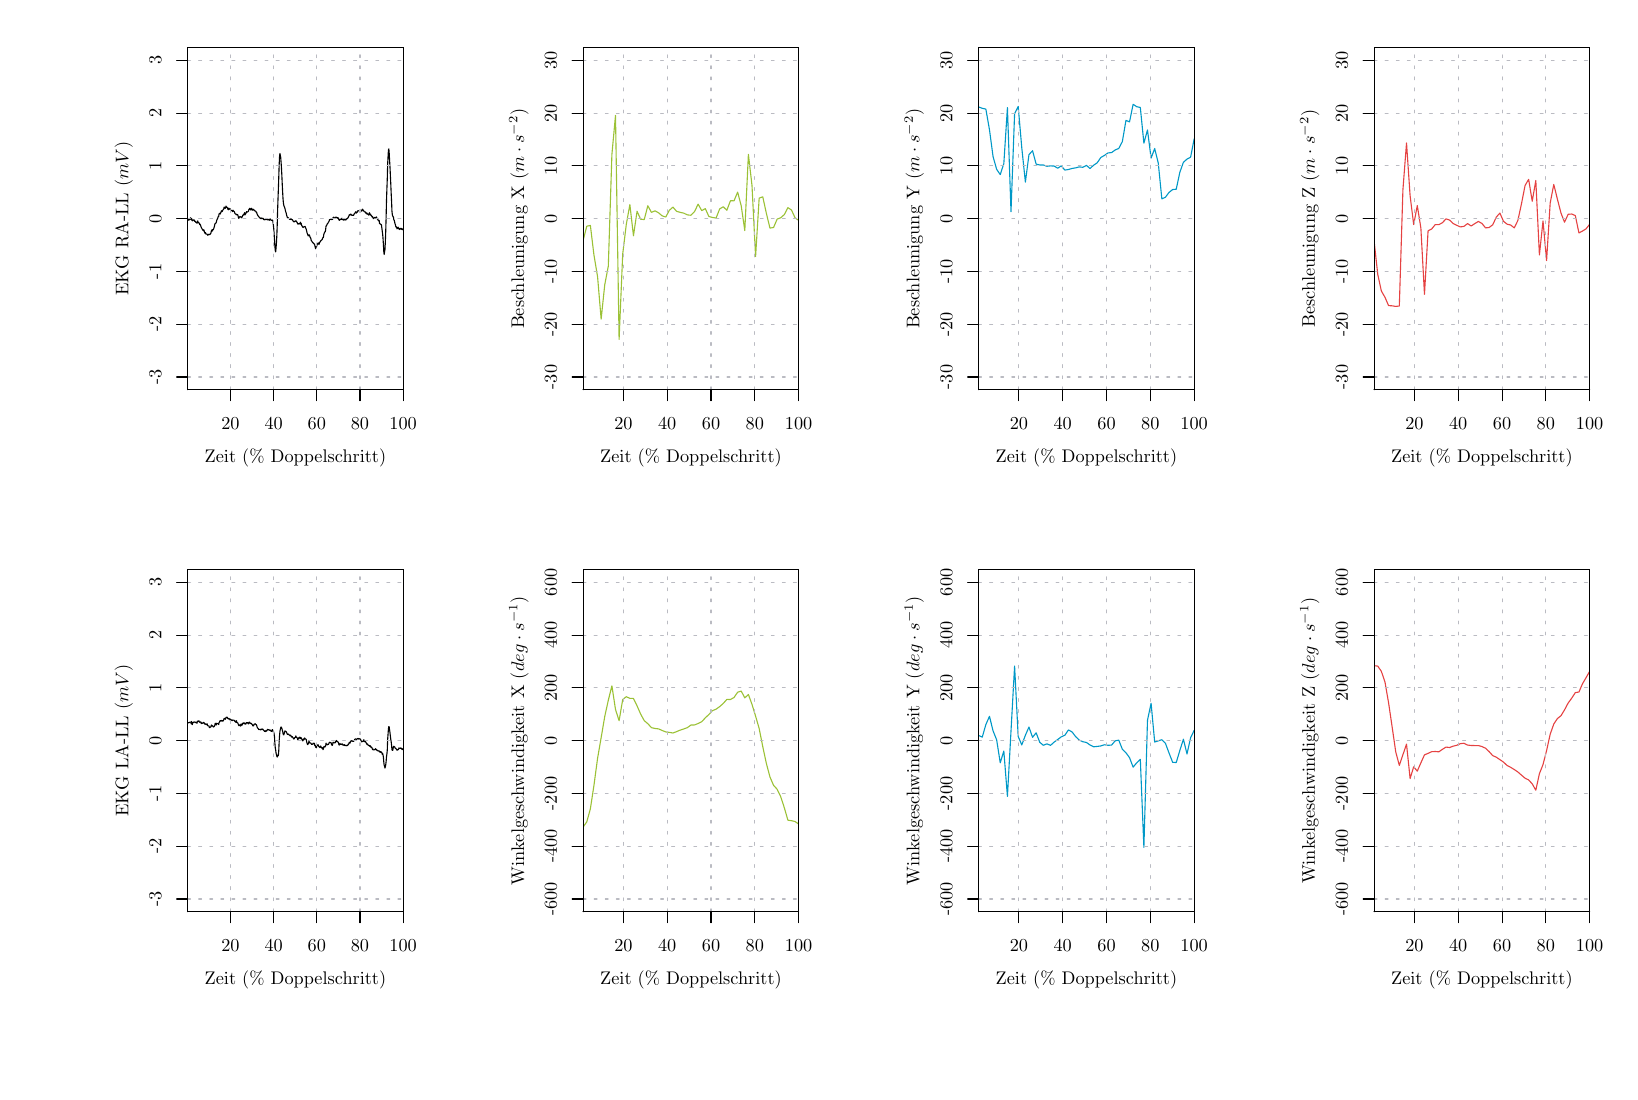
\begin{tikzpicture}[x=1pt,y=1pt]
\definecolor{fillColor}{RGB}{255,255,255}
\path[use as bounding box,fill=fillColor,fill opacity=0.00] (0,0) rectangle (571.66,377.25);
\begin{scope}
\path[clip] ( 57.82,246.44) rectangle (135.69,370.02);
\definecolor{drawColor}{RGB}{0,0,0}

\path[draw=drawColor,line width= 0.4pt,line join=round,line cap=round] ( 57.82,308.23) --
	( 57.96,308.00) --
	( 58.10,308.00) --
	( 58.24,307.59) --
	( 58.38,308.01) --
	( 58.52,307.91) --
	( 58.66,308.08) --
	( 58.80,308.55) --
	( 58.94,308.42) --
	( 59.08,307.83) --
	( 59.22,308.31) --
	( 59.36,307.76) --
	( 59.50,307.44) --
	( 59.64,307.50) --
	( 59.78,307.74) --
	( 59.92,307.83) --
	( 60.06,307.75) --
	( 60.20,307.75) --
	( 60.34,307.28) --
	( 60.48,307.27) --
	( 60.62,307.27) --
	( 60.76,306.87) --
	( 60.90,306.87) --
	( 61.04,306.89) --
	( 61.18,306.55) --
	( 61.32,307.16) --
	( 61.46,307.42) --
	( 61.60,306.79) --
	( 61.74,306.87) --
	( 61.88,306.64) --
	( 62.02,306.57) --
	( 62.16,306.07) --
	( 62.30,306.24) --
	( 62.44,305.93) --
	( 62.58,305.46) --
	( 62.72,305.06) --
	( 62.86,304.86) --
	( 63.00,304.55) --
	( 63.14,304.40) --
	( 63.28,304.08) --
	( 63.42,304.25) --
	( 63.56,303.84) --
	( 63.70,304.16) --
	( 63.84,303.53) --
	( 63.98,303.13) --
	( 64.12,302.95) --
	( 64.26,303.22) --
	( 64.40,302.63) --
	( 64.54,302.73) --
	( 64.68,302.64) --
	( 64.82,302.64) --
	( 64.96,302.50) --
	( 65.10,302.24) --
	( 65.24,302.40) --
	( 65.38,302.48) --
	( 65.52,302.64) --
	( 65.66,302.49) --
	( 65.80,302.49) --
	( 65.94,302.57) --
	( 66.08,302.81) --
	( 66.22,303.04) --
	( 66.36,303.74) --
	( 66.50,304.06) --
	( 66.64,304.23) --
	( 66.78,303.76) --
	( 66.92,304.23) --
	( 67.06,304.32) --
	( 67.20,304.52) --
	( 67.34,305.06) --
	( 67.48,305.46) --
	( 67.62,306.16) --
	( 67.76,306.47) --
	( 67.90,306.55) --
	( 68.04,306.64) --
	( 68.18,307.04) --
	( 68.32,307.59) --
	( 68.46,307.98) --
	( 68.60,308.22) --
	( 68.74,308.58) --
	( 68.88,309.11) --
	( 69.02,309.04) --
	( 69.16,309.99) --
	( 69.30,309.91) --
	( 69.44,310.23) --
	( 69.58,309.91) --
	( 69.72,310.31) --
	( 69.86,310.62) --
	( 70.00,311.09) --
	( 70.14,311.05) --
	( 70.28,310.79) --
	( 70.42,311.12) --
	( 70.56,311.43) --
	( 70.70,311.50) --
	( 70.84,311.73) --
	( 70.98,312.36) --
	( 71.12,312.38) --
	( 71.26,311.98) --
	( 71.40,311.98) --
	( 71.54,312.20) --
	( 71.68,312.78) --
	( 71.82,312.36) --
	( 71.96,312.39) --
	( 72.10,312.30) --
	( 72.24,311.91) --
	( 72.38,311.60) --
	( 72.52,311.44) --
	( 72.66,312.07) --
	( 72.80,311.91) --
	( 72.94,311.75) --
	( 73.08,311.58) --
	( 73.22,311.75) --
	( 73.36,311.33) --
	( 73.50,311.18) --
	( 73.64,311.11) --
	( 73.78,311.18) --
	( 73.92,311.12) --
	( 74.06,310.79) --
	( 74.20,311.27) --
	( 74.34,311.11) --
	( 74.48,310.95) --
	( 74.62,310.80) --
	( 74.76,310.52) --
	( 74.90,310.06) --
	( 75.04,309.99) --
	( 75.18,309.91) --
	( 75.32,309.67) --
	( 75.46,309.83) --
	( 75.60,309.58) --
	( 75.74,309.59) --
	( 75.88,309.67) --
	( 76.02,309.30) --
	( 76.16,308.60) --
	( 76.30,308.32) --
	( 76.44,308.72) --
	( 76.58,308.79) --
	( 76.72,309.03) --
	( 76.86,308.88) --
	( 77.00,308.79) --
	( 77.14,308.87) --
	( 77.28,308.55) --
	( 77.42,308.86) --
	( 77.56,308.93) --
	( 77.70,309.41) --
	( 77.84,309.44) --
	( 77.98,309.83) --
	( 78.12,309.59) --
	( 78.26,309.97) --
	( 78.40,310.41) --
	( 78.54,309.58) --
	( 78.68,309.99) --
	( 78.82,309.99) --
	( 78.96,310.44) --
	( 79.10,310.79) --
	( 79.24,310.54) --
	( 79.38,310.71) --
	( 79.52,310.71) --
	( 79.66,310.78) --
	( 79.80,311.09) --
	( 79.94,311.57) --
	( 80.08,311.67) --
	( 80.22,311.98) --
	( 80.36,311.51) --
	( 80.51,311.59) --
	( 80.65,311.32) --
	( 80.79,311.99) --
	( 80.93,311.50) --
	( 81.07,311.75) --
	( 81.21,311.51) --
	( 81.35,311.26) --
	( 81.49,311.67) --
	( 81.63,311.34) --
	( 81.77,311.42) --
	( 81.91,311.27) --
	( 82.05,311.11) --
	( 82.19,310.95) --
	( 82.33,310.95) --
	( 82.47,310.86) --
	( 82.61,310.47) --
	( 82.75,310.47) --
	( 82.89,309.94) --
	( 83.03,309.58) --
	( 83.17,309.43) --
	( 83.31,309.19) --
	( 83.45,309.03) --
	( 83.59,308.89) --
	( 83.73,308.54) --
	( 83.87,308.63) --
	( 84.01,308.47) --
	( 84.15,308.31) --
	( 84.29,308.23) --
	( 84.43,308.47) --
	( 84.57,308.23) --
	( 84.71,308.31) --
	( 84.85,308.23) --
	( 84.99,308.39) --
	( 85.13,308.26) --
	( 85.27,307.90) --
	( 85.41,307.91) --
	( 85.55,307.83) --
	( 85.69,307.91) --
	( 85.83,308.08) --
	( 85.97,307.92) --
	( 86.11,308.31) --
	( 86.25,307.91) --
	( 86.39,308.07) --
	( 86.53,308.00) --
	( 86.67,307.93) --
	( 86.81,307.76) --
	( 86.95,307.99) --
	( 87.09,307.83) --
	( 87.23,307.76) --
	( 87.37,307.66) --
	( 87.51,308.08) --
	( 87.65,308.15) --
	( 87.79,307.92) --
	( 87.93,307.76) --
	( 88.07,307.60) --
	( 88.21,307.59) --
	( 88.35,307.60) --
	( 88.49,307.75) --
	( 88.63,307.12) --
	( 88.77,306.03) --
	( 88.91,304.74) --
	( 89.05,302.68) --
	( 89.19,300.65) --
	( 89.33,298.15) --
	( 89.47,296.78) --
	( 89.61,296.22) --
	( 89.75,297.63) --
	( 89.89,299.52) --
	( 90.03,302.11) --
	( 90.17,305.76) --
	( 90.31,311.15) --
	( 90.45,315.16) --
	( 90.59,318.99) --
	( 90.73,323.20) --
	( 90.87,327.58) --
	( 91.01,330.62) --
	( 91.15,331.79) --
	( 91.29,331.11) --
	( 91.43,330.32) --
	( 91.57,328.59) --
	( 91.71,326.49) --
	( 91.85,323.79) --
	( 91.99,320.60) --
	( 92.13,317.88) --
	( 92.27,315.45) --
	( 92.41,313.87) --
	( 92.55,313.06) --
	( 92.69,312.60) --
	( 92.83,312.37) --
	( 92.97,311.89) --
	( 93.11,311.27) --
	( 93.25,310.72) --
	( 93.39,310.34) --
	( 93.53,309.66) --
	( 93.67,309.19) --
	( 93.81,308.72) --
	( 93.95,308.55) --
	( 94.09,308.55) --
	( 94.23,308.54) --
	( 94.37,308.30) --
	( 94.51,308.15) --
	( 94.65,307.99) --
	( 94.79,307.99) --
	( 94.93,308.00) --
	( 95.07,308.31) --
	( 95.21,307.91) --
	( 95.35,307.99) --
	( 95.49,307.84) --
	( 95.63,307.91) --
	( 95.77,307.65) --
	( 95.91,307.35) --
	( 96.05,307.27) --
	( 96.19,307.04) --
	( 96.33,307.10) --
	( 96.47,307.28) --
	( 96.61,307.27) --
	( 96.75,307.27) --
	( 96.89,307.51) --
	( 97.03,307.37) --
	( 97.17,307.18) --
	( 97.31,306.87) --
	( 97.45,306.71) --
	( 97.59,306.32) --
	( 97.73,306.23) --
	( 97.87,306.31) --
	( 98.01,306.48) --
	( 98.15,306.48) --
	( 98.29,306.32) --
	( 98.43,306.45) --
	( 98.57,306.97) --
	( 98.71,306.22) --
	( 98.85,306.47) --
	( 98.99,305.75) --
	( 99.13,305.68) --
	( 99.27,305.29) --
	( 99.41,305.19) --
	( 99.55,305.04) --
	( 99.69,305.28) --
	( 99.83,305.28) --
	( 99.97,305.36) --
	(100.11,305.35) --
	(100.25,305.43) --
	(100.39,304.95) --
	(100.53,304.72) --
	(100.67,304.33) --
	(100.81,303.79) --
	(100.95,303.11) --
	(101.09,302.80) --
	(101.23,302.41) --
	(101.37,302.01) --
	(101.51,302.22) --
	(101.65,302.41) --
	(101.79,302.31) --
	(101.93,301.92) --
	(102.07,301.45) --
	(102.21,301.37) --
	(102.35,300.93) --
	(102.49,300.24) --
	(102.63,300.17) --
	(102.77,299.94) --
	(102.91,299.62) --
	(103.05,299.61) --
	(103.19,299.44) --
	(103.33,299.20) --
	(103.47,299.13) --
	(103.61,299.13) --
	(103.75,298.60) --
	(103.89,297.98) --
	(104.03,297.37) --
	(104.17,297.85) --
	(104.31,298.09) --
	(104.45,298.31) --
	(104.59,298.86) --
	(104.73,299.06) --
	(104.87,299.30) --
	(105.01,299.45) --
	(105.15,299.06) --
	(105.29,298.95) --
	(105.43,299.55) --
	(105.57,299.77) --
	(105.72,299.84) --
	(105.86,300.24) --
	(106.00,300.25) --
	(106.14,300.42) --
	(106.28,300.57) --
	(106.42,300.65) --
	(106.56,301.20) --
	(106.70,301.37) --
	(106.84,301.41) --
	(106.98,302.42) --
	(107.12,302.88) --
	(107.26,303.19) --
	(107.40,303.52) --
	(107.54,303.50) --
	(107.68,304.40) --
	(107.82,305.62) --
	(107.96,305.68) --
	(108.10,305.91) --
	(108.24,306.30) --
	(108.38,306.48) --
	(108.52,306.64) --
	(108.66,306.95) --
	(108.80,307.03) --
	(108.94,307.40) --
	(109.08,307.90) --
	(109.22,307.83) --
	(109.36,307.99) --
	(109.50,307.99) --
	(109.64,308.07) --
	(109.78,307.92) --
	(109.92,307.92) --
	(110.06,308.15) --
	(110.20,307.99) --
	(110.34,308.61) --
	(110.48,308.63) --
	(110.62,308.79) --
	(110.76,308.54) --
	(110.90,308.55) --
	(111.04,308.47) --
	(111.18,308.54) --
	(111.32,308.79) --
	(111.46,308.71) --
	(111.60,308.79) --
	(111.74,308.56) --
	(111.88,308.39) --
	(112.02,308.62) --
	(112.16,308.54) --
	(112.30,308.30) --
	(112.44,307.83) --
	(112.58,307.67) --
	(112.72,307.66) --
	(112.86,308.00) --
	(113.00,308.07) --
	(113.14,307.99) --
	(113.28,307.91) --
	(113.42,308.13) --
	(113.56,308.41) --
	(113.70,307.89) --
	(113.84,307.92) --
	(113.98,308.15) --
	(114.12,307.68) --
	(114.26,307.74) --
	(114.40,307.83) --
	(114.54,307.83) --
	(114.68,307.83) --
	(114.82,307.84) --
	(114.96,307.74) --
	(115.10,308.08) --
	(115.24,308.08) --
	(115.38,308.31) --
	(115.52,308.23) --
	(115.66,308.38) --
	(115.80,308.70) --
	(115.94,308.87) --
	(116.08,309.19) --
	(116.22,309.66) --
	(116.36,309.52) --
	(116.50,309.49) --
	(116.64,309.84) --
	(116.78,309.90) --
	(116.92,309.67) --
	(117.06,309.51) --
	(117.20,309.43) --
	(117.34,309.43) --
	(117.48,309.51) --
	(117.62,309.43) --
	(117.76,309.42) --
	(117.90,309.81) --
	(118.04,309.98) --
	(118.18,310.16) --
	(118.32,310.39) --
	(118.46,310.55) --
	(118.60,310.79) --
	(118.74,310.24) --
	(118.88,310.40) --
	(119.02,310.55) --
	(119.16,310.62) --
	(119.30,311.09) --
	(119.44,311.04) --
	(119.58,311.03) --
	(119.72,311.11) --
	(119.86,311.11) --
	(120.00,311.19) --
	(120.14,311.18) --
	(120.28,311.28) --
	(120.42,310.78) --
	(120.56,311.10) --
	(120.70,311.34) --
	(120.84,311.41) --
	(120.98,311.68) --
	(121.12,311.09) --
	(121.26,311.35) --
	(121.40,311.10) --
	(121.54,310.87) --
	(121.68,310.71) --
	(121.82,310.70) --
	(121.96,310.63) --
	(122.10,310.63) --
	(122.24,310.16) --
	(122.38,310.29) --
	(122.52,310.34) --
	(122.66,309.82) --
	(122.80,309.99) --
	(122.94,309.83) --
	(123.08,309.83) --
	(123.22,309.51) --
	(123.36,309.93) --
	(123.50,310.39) --
	(123.64,309.60) --
	(123.78,309.73) --
	(123.92,309.85) --
	(124.06,309.41) --
	(124.20,309.35) --
	(124.34,309.18) --
	(124.48,308.79) --
	(124.62,308.95) --
	(124.76,308.66) --
	(124.90,308.23) --
	(125.04,308.39) --
	(125.18,308.55) --
	(125.32,308.54) --
	(125.46,308.71) --
	(125.60,308.46) --
	(125.74,308.39) --
	(125.88,308.47) --
	(126.02,308.87) --
	(126.16,308.57) --
	(126.30,308.15) --
	(126.44,308.23) --
	(126.58,307.68) --
	(126.72,307.68) --
	(126.86,307.43) --
	(127.00,307.64) --
	(127.14,306.51) --
	(127.28,306.40) --
	(127.42,306.32) --
	(127.56,306.16) --
	(127.70,306.16) --
	(127.84,305.90) --
	(127.98,304.87) --
	(128.12,303.78) --
	(128.26,302.70) --
	(128.40,301.17) --
	(128.54,298.96) --
	(128.68,296.33) --
	(128.82,295.30) --
	(128.96,296.25) --
	(129.10,297.08) --
	(129.24,299.74) --
	(129.38,303.54) --
	(129.52,308.62) --
	(129.66,314.80) --
	(129.80,318.93) --
	(129.94,322.56) --
	(130.08,327.95) --
	(130.22,330.66) --
	(130.36,332.99) --
	(130.50,333.47) --
	(130.64,331.80) --
	(130.78,329.21) --
	(130.93,326.72) --
	(131.07,323.67) --
	(131.21,320.71) --
	(131.35,317.43) --
	(131.49,314.58) --
	(131.63,310.97) --
	(131.77,309.65) --
	(131.91,309.19) --
	(132.05,308.95) --
	(132.19,308.67) --
	(132.33,307.66) --
	(132.47,307.67) --
	(132.61,306.97) --
	(132.75,306.33) --
	(132.89,306.03) --
	(133.03,305.32) --
	(133.17,305.13) --
	(133.31,305.27) --
	(133.45,304.56) --
	(133.59,304.71) --
	(133.73,304.94) --
	(133.87,305.12) --
	(134.01,304.80) --
	(134.15,304.57) --
	(134.29,304.32) --
	(134.43,304.54) --
	(134.57,304.73) --
	(134.71,304.71) --
	(134.85,304.40) --
	(134.99,304.72) --
	(135.13,304.40) --
	(135.27,304.56) --
	(135.41,304.24) --
	(135.55,304.40) --
	(135.69,304.56);
\end{scope}
\begin{scope}
\path[clip] (  0.00,  0.00) rectangle (571.66,377.25);
\definecolor{drawColor}{RGB}{0,0,0}

\path[draw=drawColor,line width= 0.4pt,line join=round,line cap=round] ( 73.28,246.44) -- (135.69,246.44);

\path[draw=drawColor,line width= 0.4pt,line join=round,line cap=round] ( 73.28,246.44) -- ( 73.28,242.48);

\path[draw=drawColor,line width= 0.4pt,line join=round,line cap=round] ( 88.88,246.44) -- ( 88.88,242.48);

\path[draw=drawColor,line width= 0.4pt,line join=round,line cap=round] (104.48,246.44) -- (104.48,242.48);

\path[draw=drawColor,line width= 0.4pt,line join=round,line cap=round] (120.08,246.44) -- (120.08,242.48);

\path[draw=drawColor,line width= 0.4pt,line join=round,line cap=round] (135.69,246.44) -- (135.69,242.48);

\node[text=drawColor,anchor=base,inner sep=0pt, outer sep=0pt, scale=  0.66] at ( 73.28,232.18) {20};

\node[text=drawColor,anchor=base,inner sep=0pt, outer sep=0pt, scale=  0.66] at ( 88.88,232.18) {40};

\node[text=drawColor,anchor=base,inner sep=0pt, outer sep=0pt, scale=  0.66] at (104.48,232.18) {60};

\node[text=drawColor,anchor=base,inner sep=0pt, outer sep=0pt, scale=  0.66] at (120.08,232.18) {80};

\node[text=drawColor,anchor=base,inner sep=0pt, outer sep=0pt, scale=  0.66] at (135.69,232.18) {100};

\path[draw=drawColor,line width= 0.4pt,line join=round,line cap=round] ( 57.82,251.02) -- ( 57.82,365.45);

\path[draw=drawColor,line width= 0.4pt,line join=round,line cap=round] ( 57.82,251.02) -- ( 53.86,251.02);

\path[draw=drawColor,line width= 0.4pt,line join=round,line cap=round] ( 57.82,270.09) -- ( 53.86,270.09);

\path[draw=drawColor,line width= 0.4pt,line join=round,line cap=round] ( 57.82,289.16) -- ( 53.86,289.16);

\path[draw=drawColor,line width= 0.4pt,line join=round,line cap=round] ( 57.82,308.23) -- ( 53.86,308.23);

\path[draw=drawColor,line width= 0.4pt,line join=round,line cap=round] ( 57.82,327.30) -- ( 53.86,327.30);

\path[draw=drawColor,line width= 0.4pt,line join=round,line cap=round] ( 57.82,346.37) -- ( 53.86,346.37);

\path[draw=drawColor,line width= 0.4pt,line join=round,line cap=round] ( 57.82,365.45) -- ( 53.86,365.45);

\node[text=drawColor,rotate= 90.00,anchor=base,inner sep=0pt, outer sep=0pt, scale=  0.66] at ( 48.31,251.02) {-3};

\node[text=drawColor,rotate= 90.00,anchor=base,inner sep=0pt, outer sep=0pt, scale=  0.66] at ( 48.31,270.09) {-2};

\node[text=drawColor,rotate= 90.00,anchor=base,inner sep=0pt, outer sep=0pt, scale=  0.66] at ( 48.31,289.16) {-1};

\node[text=drawColor,rotate= 90.00,anchor=base,inner sep=0pt, outer sep=0pt, scale=  0.66] at ( 48.31,308.23) {0};

\node[text=drawColor,rotate= 90.00,anchor=base,inner sep=0pt, outer sep=0pt, scale=  0.66] at ( 48.31,327.30) {1};

\node[text=drawColor,rotate= 90.00,anchor=base,inner sep=0pt, outer sep=0pt, scale=  0.66] at ( 48.31,346.37) {2};

\node[text=drawColor,rotate= 90.00,anchor=base,inner sep=0pt, outer sep=0pt, scale=  0.66] at ( 48.31,365.45) {3};

\path[draw=drawColor,line width= 0.4pt,line join=round,line cap=round] ( 57.82,246.44) --
	(135.69,246.44) --
	(135.69,370.02) --
	( 57.82,370.02) --
	( 57.82,246.44);
\end{scope}
\begin{scope}
\path[clip] (  0.00,188.62) rectangle (142.91,377.25);
\definecolor{drawColor}{RGB}{0,0,0}

\node[text=drawColor,anchor=base,inner sep=0pt, outer sep=0pt, scale=  0.66] at ( 96.75,220.30) {Zeit (\% Doppelschritt)};

\node[text=drawColor,rotate= 90.00,anchor=base,inner sep=0pt, outer sep=0pt, scale=  0.66] at ( 36.43,308.23) {EKG RA-LL ($mV$)};
\end{scope}
\begin{scope}
\path[clip] ( 57.82,246.44) rectangle (135.69,370.02);
\definecolor{drawColor}{RGB}{186,187,194}

\path[draw=drawColor,line width= 0.4pt,dash pattern=on 1pt off 3pt ,line join=round,line cap=round] ( 73.28,246.44) -- ( 73.28,370.02);

\path[draw=drawColor,line width= 0.4pt,dash pattern=on 1pt off 3pt ,line join=round,line cap=round] ( 88.88,246.44) -- ( 88.88,370.02);

\path[draw=drawColor,line width= 0.4pt,dash pattern=on 1pt off 3pt ,line join=round,line cap=round] (104.48,246.44) -- (104.48,370.02);

\path[draw=drawColor,line width= 0.4pt,dash pattern=on 1pt off 3pt ,line join=round,line cap=round] (120.08,246.44) -- (120.08,370.02);

\path[draw=drawColor,line width= 0.4pt,dash pattern=on 1pt off 3pt ,line join=round,line cap=round] (135.69,246.44) -- (135.69,370.02);

\path[draw=drawColor,line width= 0.4pt,dash pattern=on 1pt off 3pt ,line join=round,line cap=round] ( 57.82,251.02) -- (135.69,251.02);

\path[draw=drawColor,line width= 0.4pt,dash pattern=on 1pt off 3pt ,line join=round,line cap=round] ( 57.82,270.09) -- (135.69,270.09);

\path[draw=drawColor,line width= 0.4pt,dash pattern=on 1pt off 3pt ,line join=round,line cap=round] ( 57.82,289.16) -- (135.69,289.16);

\path[draw=drawColor,line width= 0.4pt,dash pattern=on 1pt off 3pt ,line join=round,line cap=round] ( 57.82,308.23) -- (135.69,308.23);

\path[draw=drawColor,line width= 0.4pt,dash pattern=on 1pt off 3pt ,line join=round,line cap=round] ( 57.82,327.30) -- (135.69,327.30);

\path[draw=drawColor,line width= 0.4pt,dash pattern=on 1pt off 3pt ,line join=round,line cap=round] ( 57.82,346.37) -- (135.69,346.37);

\path[draw=drawColor,line width= 0.4pt,dash pattern=on 1pt off 3pt ,line join=round,line cap=round] ( 57.82,365.45) -- (135.69,365.45);
\end{scope}
\begin{scope}
\path[clip] (  0.00,  0.00) rectangle (571.66,377.25);
\definecolor{drawColor}{RGB}{0,0,0}

\path[draw=drawColor,line width= 0.4pt,line join=round,line cap=round] ( 57.82,246.44) --
	(135.69,246.44) --
	(135.69,370.02) --
	( 57.82,370.02) --
	( 57.82,246.44);
\end{scope}
\begin{scope}
\path[clip] ( 57.82, 57.82) rectangle (135.69,181.40);
\definecolor{drawColor}{RGB}{0,0,0}

\path[draw=drawColor,line width= 0.4pt,line join=round,line cap=round] ( 57.82,126.23) --
	( 57.96,126.16) --
	( 58.10,126.07) --
	( 58.24,126.15) --
	( 58.38,126.15) --
	( 58.52,126.24) --
	( 58.66,126.31) --
	( 58.80,126.31) --
	( 58.94,126.26) --
	( 59.08,125.69) --
	( 59.22,126.56) --
	( 59.36,125.76) --
	( 59.50,125.43) --
	( 59.64,125.97) --
	( 59.78,126.15) --
	( 59.92,126.24) --
	( 60.06,126.39) --
	( 60.20,126.31) --
	( 60.34,126.39) --
	( 60.48,126.16) --
	( 60.62,126.16) --
	( 60.76,126.31) --
	( 60.90,126.16) --
	( 61.04,126.08) --
	( 61.18,125.89) --
	( 61.32,126.59) --
	( 61.46,126.71) --
	( 61.60,126.63) --
	( 61.74,126.55) --
	( 61.88,126.80) --
	( 62.02,126.34) --
	( 62.16,126.24) --
	( 62.30,126.39) --
	( 62.44,126.39) --
	( 62.58,126.34) --
	( 62.72,125.76) --
	( 62.86,126.09) --
	( 63.00,125.91) --
	( 63.14,125.91) --
	( 63.28,125.99) --
	( 63.42,125.99) --
	( 63.56,126.24) --
	( 63.70,126.15) --
	( 63.84,125.84) --
	( 63.98,125.59) --
	( 64.12,125.75) --
	( 64.26,125.53) --
	( 64.40,125.52) --
	( 64.54,125.43) --
	( 64.68,125.36) --
	( 64.82,125.75) --
	( 64.96,125.30) --
	( 65.10,124.95) --
	( 65.24,124.96) --
	( 65.38,124.96) --
	( 65.52,124.89) --
	( 65.66,124.34) --
	( 65.80,124.33) --
	( 65.94,124.48) --
	( 66.08,124.56) --
	( 66.22,124.55) --
	( 66.36,125.27) --
	( 66.50,124.97) --
	( 66.64,125.12) --
	( 66.78,124.96) --
	( 66.92,124.80) --
	( 67.06,124.57) --
	( 67.20,124.55) --
	( 67.34,124.73) --
	( 67.48,124.88) --
	( 67.62,125.20) --
	( 67.76,125.91) --
	( 67.90,125.37) --
	( 68.04,125.51) --
	( 68.18,125.28) --
	( 68.32,125.91) --
	( 68.46,125.76) --
	( 68.60,125.75) --
	( 68.74,125.76) --
	( 68.88,125.66) --
	( 69.02,125.44) --
	( 69.16,126.15) --
	( 69.30,126.31) --
	( 69.44,126.69) --
	( 69.58,126.87) --
	( 69.72,126.79) --
	( 69.86,126.63) --
	( 70.00,126.94) --
	( 70.14,126.88) --
	( 70.28,126.86) --
	( 70.42,126.63) --
	( 70.56,126.71) --
	( 70.70,126.79) --
	( 70.84,127.18) --
	( 70.98,127.58) --
	( 71.12,127.67) --
	( 71.26,127.51) --
	( 71.40,127.35) --
	( 71.54,127.57) --
	( 71.68,128.06) --
	( 71.82,127.99) --
	( 71.96,128.15) --
	( 72.10,128.07) --
	( 72.24,127.67) --
	( 72.38,127.68) --
	( 72.52,127.43) --
	( 72.66,127.67) --
	( 72.80,127.51) --
	( 72.94,127.44) --
	( 73.08,127.11) --
	( 73.22,127.42) --
	( 73.36,127.17) --
	( 73.50,126.87) --
	( 73.64,127.11) --
	( 73.78,127.11) --
	( 73.92,127.04) --
	( 74.06,126.87) --
	( 74.20,127.03) --
	( 74.34,127.03) --
	( 74.48,127.03) --
	( 74.62,126.95) --
	( 74.76,126.85) --
	( 74.90,126.47) --
	( 75.04,126.63) --
	( 75.18,126.32) --
	( 75.32,126.22) --
	( 75.46,126.79) --
	( 75.60,126.22) --
	( 75.74,126.07) --
	( 75.88,126.08) --
	( 76.02,125.77) --
	( 76.16,125.39) --
	( 76.30,125.03) --
	( 76.44,125.20) --
	( 76.58,125.20) --
	( 76.72,125.36) --
	( 76.86,124.90) --
	( 77.00,124.90) --
	( 77.14,125.68) --
	( 77.28,125.28) --
	( 77.42,125.19) --
	( 77.56,125.41) --
	( 77.70,125.81) --
	( 77.84,126.00) --
	( 77.98,126.07) --
	( 78.12,125.75) --
	( 78.26,125.91) --
	( 78.40,126.01) --
	( 78.54,125.59) --
	( 78.68,125.59) --
	( 78.82,125.59) --
	( 78.96,125.98) --
	( 79.10,126.16) --
	( 79.24,125.99) --
	( 79.38,126.08) --
	( 79.52,126.07) --
	( 79.66,125.76) --
	( 79.80,125.67) --
	( 79.94,126.13) --
	( 80.08,126.32) --
	( 80.22,126.31) --
	( 80.36,125.92) --
	( 80.51,125.83) --
	( 80.65,125.83) --
	( 80.79,125.91) --
	( 80.93,125.67) --
	( 81.07,125.51) --
	( 81.21,125.36) --
	( 81.35,124.96) --
	( 81.49,125.04) --
	( 81.63,124.96) --
	( 81.77,125.43) --
	( 81.91,125.60) --
	( 82.05,125.59) --
	( 82.19,125.75) --
	( 82.33,125.58) --
	( 82.47,125.43) --
	( 82.61,125.36) --
	( 82.75,125.13) --
	( 82.89,124.58) --
	( 83.03,124.23) --
	( 83.17,124.08) --
	( 83.31,124.00) --
	( 83.45,123.69) --
	( 83.59,123.59) --
	( 83.73,123.68) --
	( 83.87,123.68) --
	( 84.01,123.68) --
	( 84.15,123.52) --
	( 84.29,123.67) --
	( 84.43,123.77) --
	( 84.57,123.60) --
	( 84.71,123.84) --
	( 84.85,123.68) --
	( 84.99,123.76) --
	( 85.13,123.46) --
	( 85.27,123.36) --
	( 85.41,123.27) --
	( 85.55,122.96) --
	( 85.69,123.12) --
	( 85.83,123.13) --
	( 85.97,122.88) --
	( 86.11,123.28) --
	( 86.25,123.12) --
	( 86.39,123.11) --
	( 86.53,123.42) --
	( 86.67,123.68) --
	( 86.81,123.52) --
	( 86.95,123.60) --
	( 87.09,123.52) --
	( 87.23,123.52) --
	( 87.37,123.36) --
	( 87.51,123.52) --
	( 87.65,123.36) --
	( 87.79,123.20) --
	( 87.93,123.13) --
	( 88.07,122.95) --
	( 88.21,123.30) --
	( 88.35,123.45) --
	( 88.49,123.59) --
	( 88.63,122.97) --
	( 88.77,122.72) --
	( 88.91,122.74) --
	( 89.05,121.98) --
	( 89.19,120.97) --
	( 89.33,118.71) --
	( 89.47,117.02) --
	( 89.61,116.24) --
	( 89.75,115.16) --
	( 89.89,114.56) --
	( 90.03,114.01) --
	( 90.17,113.69) --
	( 90.31,114.41) --
	( 90.45,114.08) --
	( 90.59,114.27) --
	( 90.73,115.99) --
	( 90.87,119.11) --
	( 91.01,121.34) --
	( 91.15,122.95) --
	( 91.29,123.63) --
	( 91.43,124.33) --
	( 91.57,124.56) --
	( 91.71,124.32) --
	( 91.85,124.10) --
	( 91.99,123.50) --
	( 92.13,123.12) --
	( 92.27,122.26) --
	( 92.41,121.77) --
	( 92.55,121.67) --
	( 92.69,122.20) --
	( 92.83,122.74) --
	( 92.97,123.12) --
	( 93.11,123.04) --
	( 93.25,122.96) --
	( 93.39,122.89) --
	( 93.53,122.63) --
	( 93.67,122.32) --
	( 93.81,121.93) --
	( 93.95,121.92) --
	( 94.09,122.00) --
	( 94.23,121.99) --
	( 94.37,121.76) --
	( 94.51,121.68) --
	( 94.65,121.61) --
	( 94.79,121.36) --
	( 94.93,121.61) --
	( 95.07,121.52) --
	( 95.21,121.29) --
	( 95.35,120.89) --
	( 95.49,120.87) --
	( 95.63,121.05) --
	( 95.77,120.79) --
	( 95.91,120.56) --
	( 96.05,120.49) --
	( 96.19,120.17) --
	( 96.33,120.39) --
	( 96.47,120.73) --
	( 96.61,120.72) --
	( 96.75,120.80) --
	( 96.89,121.36) --
	( 97.03,120.91) --
	( 97.17,120.80) --
	( 97.31,120.72) --
	( 97.45,120.48) --
	( 97.59,119.93) --
	( 97.73,120.15) --
	( 97.87,120.56) --
	( 98.01,120.57) --
	( 98.15,120.88) --
	( 98.29,120.74) --
	( 98.43,120.32) --
	( 98.57,120.79) --
	( 98.71,120.64) --
	( 98.85,120.64) --
	( 98.99,120.16) --
	( 99.13,120.17) --
	( 99.27,119.63) --
	( 99.41,119.53) --
	( 99.55,119.85) --
	( 99.69,120.25) --
	( 99.83,119.93) --
	( 99.97,120.37) --
	(100.11,120.58) --
	(100.25,120.32) --
	(100.39,120.24) --
	(100.53,120.17) --
	(100.67,119.94) --
	(100.81,119.24) --
	(100.95,118.71) --
	(101.09,118.25) --
	(101.23,118.16) --
	(101.37,118.57) --
	(101.51,118.60) --
	(101.65,119.62) --
	(101.79,118.87) --
	(101.93,118.97) --
	(102.07,118.73) --
	(102.21,118.73) --
	(102.35,118.74) --
	(102.49,118.40) --
	(102.63,118.25) --
	(102.77,118.25) --
	(102.91,118.41) --
	(103.05,118.39) --
	(103.19,118.73) --
	(103.33,118.40) --
	(103.47,118.65) --
	(103.61,118.66) --
	(103.75,117.86) --
	(103.89,118.00) --
	(104.03,117.28) --
	(104.17,117.21) --
	(104.31,117.05) --
	(104.45,117.49) --
	(104.59,118.08) --
	(104.73,117.93) --
	(104.87,118.10) --
	(105.01,118.09) --
	(105.15,117.62) --
	(105.29,117.38) --
	(105.43,117.29) --
	(105.57,117.13) --
	(105.72,117.28) --
	(105.86,117.69) --
	(106.00,117.39) --
	(106.14,117.20) --
	(106.28,116.89) --
	(106.42,116.98) --
	(106.56,117.06) --
	(106.70,116.35) --
	(106.84,116.61) --
	(106.98,117.30) --
	(107.12,117.53) --
	(107.26,117.54) --
	(107.40,117.29) --
	(107.54,117.52) --
	(107.68,117.74) --
	(107.82,118.74) --
	(107.96,118.17) --
	(108.10,118.17) --
	(108.24,118.33) --
	(108.38,118.09) --
	(108.52,118.25) --
	(108.66,118.25) --
	(108.80,118.48) --
	(108.94,118.87) --
	(109.08,119.05) --
	(109.22,118.89) --
	(109.36,118.97) --
	(109.50,118.89) --
	(109.64,118.90) --
	(109.78,118.28) --
	(109.92,118.01) --
	(110.06,117.93) --
	(110.20,118.24) --
	(110.34,119.03) --
	(110.48,118.97) --
	(110.62,119.04) --
	(110.76,118.80) --
	(110.90,118.81) --
	(111.04,118.81) --
	(111.18,118.95) --
	(111.32,119.44) --
	(111.46,119.37) --
	(111.60,119.69) --
	(111.74,119.30) --
	(111.88,119.28) --
	(112.02,119.30) --
	(112.16,119.04) --
	(112.30,118.88) --
	(112.44,118.25) --
	(112.58,118.01) --
	(112.72,118.23) --
	(112.86,118.57) --
	(113.00,118.25) --
	(113.14,118.33) --
	(113.28,118.25) --
	(113.42,118.24) --
	(113.56,118.48) --
	(113.70,118.40) --
	(113.84,118.08) --
	(113.98,118.01) --
	(114.12,118.09) --
	(114.26,117.93) --
	(114.40,118.17) --
	(114.54,117.93) --
	(114.68,117.85) --
	(114.82,117.93) --
	(114.96,117.94) --
	(115.10,117.77) --
	(115.24,117.93) --
	(115.38,117.85) --
	(115.52,117.85) --
	(115.66,117.92) --
	(115.80,118.32) --
	(115.94,118.25) --
	(116.08,118.65) --
	(116.22,118.97) --
	(116.36,118.74) --
	(116.50,118.69) --
	(116.64,119.39) --
	(116.78,119.45) --
	(116.92,119.61) --
	(117.06,119.53) --
	(117.20,119.37) --
	(117.34,119.45) --
	(117.48,119.53) --
	(117.62,119.37) --
	(117.76,119.36) --
	(117.90,119.52) --
	(118.04,119.74) --
	(118.18,120.10) --
	(118.32,120.17) --
	(118.46,120.25) --
	(118.60,120.25) --
	(118.74,120.01) --
	(118.88,120.01) --
	(119.02,120.17) --
	(119.16,120.32) --
	(119.30,120.40) --
	(119.44,120.41) --
	(119.58,120.23) --
	(119.72,120.17) --
	(119.86,120.25) --
	(120.00,120.33) --
	(120.14,120.17) --
	(120.28,120.18) --
	(120.42,119.60) --
	(120.56,119.53) --
	(120.70,119.21) --
	(120.84,119.28) --
	(120.98,119.29) --
	(121.12,119.29) --
	(121.26,119.54) --
	(121.40,119.93) --
	(121.54,119.86) --
	(121.68,119.21) --
	(121.82,119.61) --
	(121.96,119.36) --
	(122.10,119.29) --
	(122.24,118.82) --
	(122.38,118.81) --
	(122.52,118.45) --
	(122.66,118.17) --
	(122.80,118.41) --
	(122.94,118.17) --
	(123.08,117.93) --
	(123.22,117.85) --
	(123.36,117.85) --
	(123.50,117.85) --
	(123.64,117.53) --
	(123.78,117.76) --
	(123.92,117.56) --
	(124.06,117.20) --
	(124.20,117.30) --
	(124.34,117.21) --
	(124.48,116.82) --
	(124.62,116.41) --
	(124.76,116.58) --
	(124.90,116.25) --
	(125.04,116.33) --
	(125.18,116.25) --
	(125.32,116.40) --
	(125.46,116.50) --
	(125.60,116.42) --
	(125.74,116.73) --
	(125.88,116.41) --
	(126.02,116.17) --
	(126.16,116.33) --
	(126.30,116.08) --
	(126.44,115.93) --
	(126.58,116.01) --
	(126.72,115.94) --
	(126.86,115.85) --
	(127.00,115.95) --
	(127.14,115.53) --
	(127.28,115.61) --
	(127.42,115.38) --
	(127.56,115.69) --
	(127.70,115.55) --
	(127.84,115.45) --
	(127.98,115.21) --
	(128.12,114.66) --
	(128.26,114.98) --
	(128.40,114.46) --
	(128.54,113.69) --
	(128.68,111.87) --
	(128.82,110.74) --
	(128.96,110.35) --
	(129.10,109.71) --
	(129.24,110.15) --
	(129.38,110.84) --
	(129.52,112.02) --
	(129.66,113.82) --
	(129.80,114.70) --
	(129.94,116.18) --
	(130.08,120.10) --
	(130.22,121.97) --
	(130.36,123.85) --
	(130.50,124.71) --
	(130.64,124.51) --
	(130.78,123.48) --
	(130.93,122.38) --
	(131.07,121.14) --
	(131.21,120.04) --
	(131.35,119.18) --
	(131.49,117.99) --
	(131.63,116.36) --
	(131.77,116.09) --
	(131.91,116.09) --
	(132.05,116.79) --
	(132.19,117.51) --
	(132.33,117.61) --
	(132.47,117.45) --
	(132.61,117.38) --
	(132.75,116.98) --
	(132.89,116.90) --
	(133.03,116.72) --
	(133.17,116.65) --
	(133.31,116.41) --
	(133.45,116.18) --
	(133.59,116.17) --
	(133.73,116.40) --
	(133.87,116.49) --
	(134.01,116.41) --
	(134.15,116.96) --
	(134.29,116.82) --
	(134.43,116.80) --
	(134.57,116.98) --
	(134.71,116.97) --
	(134.85,116.81) --
	(134.99,116.89) --
	(135.13,116.58) --
	(135.27,116.65) --
	(135.41,116.41) --
	(135.55,116.41) --
	(135.69,116.81);
\end{scope}
\begin{scope}
\path[clip] (  0.00,  0.00) rectangle (571.66,377.25);
\definecolor{drawColor}{RGB}{0,0,0}

\path[draw=drawColor,line width= 0.4pt,line join=round,line cap=round] ( 73.28, 57.82) -- (135.69, 57.82);

\path[draw=drawColor,line width= 0.4pt,line join=round,line cap=round] ( 73.28, 57.82) -- ( 73.28, 53.86);

\path[draw=drawColor,line width= 0.4pt,line join=round,line cap=round] ( 88.88, 57.82) -- ( 88.88, 53.86);

\path[draw=drawColor,line width= 0.4pt,line join=round,line cap=round] (104.48, 57.82) -- (104.48, 53.86);

\path[draw=drawColor,line width= 0.4pt,line join=round,line cap=round] (120.08, 57.82) -- (120.08, 53.86);

\path[draw=drawColor,line width= 0.4pt,line join=round,line cap=round] (135.69, 57.82) -- (135.69, 53.86);

\node[text=drawColor,anchor=base,inner sep=0pt, outer sep=0pt, scale=  0.66] at ( 73.28, 43.56) {20};

\node[text=drawColor,anchor=base,inner sep=0pt, outer sep=0pt, scale=  0.66] at ( 88.88, 43.56) {40};

\node[text=drawColor,anchor=base,inner sep=0pt, outer sep=0pt, scale=  0.66] at (104.48, 43.56) {60};

\node[text=drawColor,anchor=base,inner sep=0pt, outer sep=0pt, scale=  0.66] at (120.08, 43.56) {80};

\node[text=drawColor,anchor=base,inner sep=0pt, outer sep=0pt, scale=  0.66] at (135.69, 43.56) {100};

\path[draw=drawColor,line width= 0.4pt,line join=round,line cap=round] ( 57.82, 62.39) -- ( 57.82,176.82);

\path[draw=drawColor,line width= 0.4pt,line join=round,line cap=round] ( 57.82, 62.39) -- ( 53.86, 62.39);

\path[draw=drawColor,line width= 0.4pt,line join=round,line cap=round] ( 57.82, 81.46) -- ( 53.86, 81.46);

\path[draw=drawColor,line width= 0.4pt,line join=round,line cap=round] ( 57.82,100.54) -- ( 53.86,100.54);

\path[draw=drawColor,line width= 0.4pt,line join=round,line cap=round] ( 57.82,119.61) -- ( 53.86,119.61);

\path[draw=drawColor,line width= 0.4pt,line join=round,line cap=round] ( 57.82,138.68) -- ( 53.86,138.68);

\path[draw=drawColor,line width= 0.4pt,line join=round,line cap=round] ( 57.82,157.75) -- ( 53.86,157.75);

\path[draw=drawColor,line width= 0.4pt,line join=round,line cap=round] ( 57.82,176.82) -- ( 53.86,176.82);

\node[text=drawColor,rotate= 90.00,anchor=base,inner sep=0pt, outer sep=0pt, scale=  0.66] at ( 48.31, 62.39) {-3};

\node[text=drawColor,rotate= 90.00,anchor=base,inner sep=0pt, outer sep=0pt, scale=  0.66] at ( 48.31, 81.46) {-2};

\node[text=drawColor,rotate= 90.00,anchor=base,inner sep=0pt, outer sep=0pt, scale=  0.66] at ( 48.31,100.54) {-1};

\node[text=drawColor,rotate= 90.00,anchor=base,inner sep=0pt, outer sep=0pt, scale=  0.66] at ( 48.31,119.61) {0};

\node[text=drawColor,rotate= 90.00,anchor=base,inner sep=0pt, outer sep=0pt, scale=  0.66] at ( 48.31,138.68) {1};

\node[text=drawColor,rotate= 90.00,anchor=base,inner sep=0pt, outer sep=0pt, scale=  0.66] at ( 48.31,157.75) {2};

\node[text=drawColor,rotate= 90.00,anchor=base,inner sep=0pt, outer sep=0pt, scale=  0.66] at ( 48.31,176.82) {3};

\path[draw=drawColor,line width= 0.4pt,line join=round,line cap=round] ( 57.82, 57.82) --
	(135.69, 57.82) --
	(135.69,181.40) --
	( 57.82,181.40) --
	( 57.82, 57.82);
\end{scope}
\begin{scope}
\path[clip] (  0.00,  0.00) rectangle (142.91,188.62);
\definecolor{drawColor}{RGB}{0,0,0}

\node[text=drawColor,anchor=base,inner sep=0pt, outer sep=0pt, scale=  0.66] at ( 96.75, 31.68) {Zeit (\% Doppelschritt)};

\node[text=drawColor,rotate= 90.00,anchor=base,inner sep=0pt, outer sep=0pt, scale=  0.66] at ( 36.43,119.61) {EKG LA-LL ($mV$)};
\end{scope}
\begin{scope}
\path[clip] ( 57.82, 57.82) rectangle (135.69,181.40);
\definecolor{drawColor}{RGB}{186,187,194}

\path[draw=drawColor,line width= 0.4pt,dash pattern=on 1pt off 3pt ,line join=round,line cap=round] ( 73.28, 57.82) -- ( 73.28,181.40);

\path[draw=drawColor,line width= 0.4pt,dash pattern=on 1pt off 3pt ,line join=round,line cap=round] ( 88.88, 57.82) -- ( 88.88,181.40);

\path[draw=drawColor,line width= 0.4pt,dash pattern=on 1pt off 3pt ,line join=round,line cap=round] (104.48, 57.82) -- (104.48,181.40);

\path[draw=drawColor,line width= 0.4pt,dash pattern=on 1pt off 3pt ,line join=round,line cap=round] (120.08, 57.82) -- (120.08,181.40);

\path[draw=drawColor,line width= 0.4pt,dash pattern=on 1pt off 3pt ,line join=round,line cap=round] (135.69, 57.82) -- (135.69,181.40);

\path[draw=drawColor,line width= 0.4pt,dash pattern=on 1pt off 3pt ,line join=round,line cap=round] ( 57.82, 62.39) -- (135.69, 62.39);

\path[draw=drawColor,line width= 0.4pt,dash pattern=on 1pt off 3pt ,line join=round,line cap=round] ( 57.82, 81.46) -- (135.69, 81.46);

\path[draw=drawColor,line width= 0.4pt,dash pattern=on 1pt off 3pt ,line join=round,line cap=round] ( 57.82,100.54) -- (135.69,100.54);

\path[draw=drawColor,line width= 0.4pt,dash pattern=on 1pt off 3pt ,line join=round,line cap=round] ( 57.82,119.61) -- (135.69,119.61);

\path[draw=drawColor,line width= 0.4pt,dash pattern=on 1pt off 3pt ,line join=round,line cap=round] ( 57.82,138.68) -- (135.69,138.68);

\path[draw=drawColor,line width= 0.4pt,dash pattern=on 1pt off 3pt ,line join=round,line cap=round] ( 57.82,157.75) -- (135.69,157.75);

\path[draw=drawColor,line width= 0.4pt,dash pattern=on 1pt off 3pt ,line join=round,line cap=round] ( 57.82,176.82) -- (135.69,176.82);
\end{scope}
\begin{scope}
\path[clip] (  0.00,  0.00) rectangle (571.66,377.25);
\definecolor{drawColor}{RGB}{0,0,0}

\path[draw=drawColor,line width= 0.4pt,line join=round,line cap=round] ( 57.82, 57.82) --
	(135.69, 57.82) --
	(135.69,181.40) --
	( 57.82,181.40) --
	( 57.82, 57.82);
\end{scope}
\begin{scope}
\path[clip] (200.73,246.44) rectangle (278.60,370.02);
\definecolor{drawColor}{RGB}{155,193,54}

\path[draw=drawColor,line width= 0.4pt,line join=round,line cap=round] (200.73,300.47) --
	(202.03,305.50) --
	(203.33,305.79) --
	(204.62,295.09) --
	(205.92,287.37) --
	(207.22,271.92) --
	(208.52,284.33) --
	(209.81,291.09) --
	(211.11,331.44) --
	(212.41,345.57) --
	(213.71,264.61) --
	(215.01,295.43) --
	(216.30,306.10) --
	(217.60,313.33) --
	(218.90,302.06) --
	(220.20,310.90) --
	(221.50,308.02) --
	(222.79,307.90) --
	(224.09,312.90) --
	(225.39,310.51) --
	(226.69,311.06) --
	(227.98,310.34) --
	(229.28,309.24) --
	(230.58,308.83) --
	(231.88,311.28) --
	(233.18,312.40) --
	(234.47,310.89) --
	(235.77,310.52) --
	(237.07,310.23) --
	(238.37,309.59) --
	(239.67,309.47) --
	(240.96,310.76) --
	(242.26,313.49) --
	(243.56,311.15) --
	(244.86,311.85) --
	(246.15,309.02) --
	(247.45,308.66) --
	(248.75,308.47) --
	(250.05,311.75) --
	(251.35,312.53) --
	(252.64,311.26) --
	(253.94,314.70) --
	(255.24,314.68) --
	(256.54,317.83) --
	(257.84,312.86) --
	(259.13,303.92) --
	(260.43,331.47) --
	(261.73,320.24) --
	(263.03,294.53) --
	(264.32,315.64) --
	(265.62,316.14) --
	(266.92,310.16) --
	(268.22,304.82) --
	(269.52,305.04) --
	(270.81,308.06) --
	(272.11,308.56) --
	(273.41,309.70) --
	(274.71,312.23) --
	(276.01,311.33) --
	(277.30,308.53) --
	(278.60,307.60);
\end{scope}
\begin{scope}
\path[clip] (  0.00,  0.00) rectangle (571.66,377.25);
\definecolor{drawColor}{RGB}{0,0,0}

\path[draw=drawColor,line width= 0.4pt,line join=round,line cap=round] (215.27,246.44) -- (278.60,246.44);

\path[draw=drawColor,line width= 0.4pt,line join=round,line cap=round] (215.27,246.44) -- (215.27,242.48);

\path[draw=drawColor,line width= 0.4pt,line join=round,line cap=round] (231.10,246.44) -- (231.10,242.48);

\path[draw=drawColor,line width= 0.4pt,line join=round,line cap=round] (246.93,246.44) -- (246.93,242.48);

\path[draw=drawColor,line width= 0.4pt,line join=round,line cap=round] (262.77,246.44) -- (262.77,242.48);

\path[draw=drawColor,line width= 0.4pt,line join=round,line cap=round] (278.60,246.44) -- (278.60,242.48);

\node[text=drawColor,anchor=base,inner sep=0pt, outer sep=0pt, scale=  0.66] at (215.27,232.18) {20};

\node[text=drawColor,anchor=base,inner sep=0pt, outer sep=0pt, scale=  0.66] at (231.10,232.18) {40};

\node[text=drawColor,anchor=base,inner sep=0pt, outer sep=0pt, scale=  0.66] at (246.93,232.18) {60};

\node[text=drawColor,anchor=base,inner sep=0pt, outer sep=0pt, scale=  0.66] at (262.77,232.18) {80};

\node[text=drawColor,anchor=base,inner sep=0pt, outer sep=0pt, scale=  0.66] at (278.60,232.18) {100};

\path[draw=drawColor,line width= 0.4pt,line join=round,line cap=round] (200.73,251.02) -- (200.73,365.45);

\path[draw=drawColor,line width= 0.4pt,line join=round,line cap=round] (200.73,251.02) -- (196.77,251.02);

\path[draw=drawColor,line width= 0.4pt,line join=round,line cap=round] (200.73,270.09) -- (196.77,270.09);

\path[draw=drawColor,line width= 0.4pt,line join=round,line cap=round] (200.73,289.16) -- (196.77,289.16);

\path[draw=drawColor,line width= 0.4pt,line join=round,line cap=round] (200.73,308.23) -- (196.77,308.23);

\path[draw=drawColor,line width= 0.4pt,line join=round,line cap=round] (200.73,327.30) -- (196.77,327.30);

\path[draw=drawColor,line width= 0.4pt,line join=round,line cap=round] (200.73,346.37) -- (196.77,346.37);

\path[draw=drawColor,line width= 0.4pt,line join=round,line cap=round] (200.73,365.45) -- (196.77,365.45);

\node[text=drawColor,rotate= 90.00,anchor=base,inner sep=0pt, outer sep=0pt, scale=  0.66] at (191.23,251.02) {-30};

\node[text=drawColor,rotate= 90.00,anchor=base,inner sep=0pt, outer sep=0pt, scale=  0.66] at (191.23,270.09) {-20};

\node[text=drawColor,rotate= 90.00,anchor=base,inner sep=0pt, outer sep=0pt, scale=  0.66] at (191.23,289.16) {-10};

\node[text=drawColor,rotate= 90.00,anchor=base,inner sep=0pt, outer sep=0pt, scale=  0.66] at (191.23,308.23) {0};

\node[text=drawColor,rotate= 90.00,anchor=base,inner sep=0pt, outer sep=0pt, scale=  0.66] at (191.23,327.30) {10};

\node[text=drawColor,rotate= 90.00,anchor=base,inner sep=0pt, outer sep=0pt, scale=  0.66] at (191.23,346.37) {20};

\node[text=drawColor,rotate= 90.00,anchor=base,inner sep=0pt, outer sep=0pt, scale=  0.66] at (191.23,365.45) {30};

\path[draw=drawColor,line width= 0.4pt,line join=round,line cap=round] (200.73,246.44) --
	(278.60,246.44) --
	(278.60,370.02) --
	(200.73,370.02) --
	(200.73,246.44);
\end{scope}
\begin{scope}
\path[clip] (142.91,188.62) rectangle (285.83,377.25);
\definecolor{drawColor}{RGB}{0,0,0}

\node[text=drawColor,anchor=base,inner sep=0pt, outer sep=0pt, scale=  0.66] at (239.67,220.30) {Zeit (\% Doppelschritt)};

\node[text=drawColor,rotate= 90.00,anchor=base,inner sep=0pt, outer sep=0pt, scale=  0.66] at (179.35,308.23) {Beschleunigung X ($m \cdot s^{-2}$)};
\end{scope}
\begin{scope}
\path[clip] (200.73,246.44) rectangle (278.60,370.02);
\definecolor{drawColor}{RGB}{186,187,194}

\path[draw=drawColor,line width= 0.4pt,dash pattern=on 1pt off 3pt ,line join=round,line cap=round] (215.27,246.44) -- (215.27,370.02);

\path[draw=drawColor,line width= 0.4pt,dash pattern=on 1pt off 3pt ,line join=round,line cap=round] (231.10,246.44) -- (231.10,370.02);

\path[draw=drawColor,line width= 0.4pt,dash pattern=on 1pt off 3pt ,line join=round,line cap=round] (246.93,246.44) -- (246.93,370.02);

\path[draw=drawColor,line width= 0.4pt,dash pattern=on 1pt off 3pt ,line join=round,line cap=round] (262.77,246.44) -- (262.77,370.02);

\path[draw=drawColor,line width= 0.4pt,dash pattern=on 1pt off 3pt ,line join=round,line cap=round] (278.60,246.44) -- (278.60,370.02);

\path[draw=drawColor,line width= 0.4pt,dash pattern=on 1pt off 3pt ,line join=round,line cap=round] (200.73,251.02) -- (278.60,251.02);

\path[draw=drawColor,line width= 0.4pt,dash pattern=on 1pt off 3pt ,line join=round,line cap=round] (200.73,270.09) -- (278.60,270.09);

\path[draw=drawColor,line width= 0.4pt,dash pattern=on 1pt off 3pt ,line join=round,line cap=round] (200.73,289.16) -- (278.60,289.16);

\path[draw=drawColor,line width= 0.4pt,dash pattern=on 1pt off 3pt ,line join=round,line cap=round] (200.73,308.23) -- (278.60,308.23);

\path[draw=drawColor,line width= 0.4pt,dash pattern=on 1pt off 3pt ,line join=round,line cap=round] (200.73,327.30) -- (278.60,327.30);

\path[draw=drawColor,line width= 0.4pt,dash pattern=on 1pt off 3pt ,line join=round,line cap=round] (200.73,346.37) -- (278.60,346.37);

\path[draw=drawColor,line width= 0.4pt,dash pattern=on 1pt off 3pt ,line join=round,line cap=round] (200.73,365.45) -- (278.60,365.45);
\end{scope}
\begin{scope}
\path[clip] (  0.00,  0.00) rectangle (571.66,377.25);
\definecolor{drawColor}{RGB}{0,0,0}

\path[draw=drawColor,line width= 0.4pt,line join=round,line cap=round] (200.73,246.44) --
	(278.60,246.44) --
	(278.60,370.02) --
	(200.73,370.02) --
	(200.73,246.44);
\end{scope}
\begin{scope}
\path[clip] (200.73, 57.82) rectangle (278.60,181.40);
\definecolor{drawColor}{RGB}{155,193,54}

\path[draw=drawColor,line width= 0.4pt,line join=round,line cap=round] (200.73, 88.43) --
	(202.03, 90.27) --
	(203.33, 94.99) --
	(204.62,103.45) --
	(205.92,113.16) --
	(207.22,120.68) --
	(208.52,128.34) --
	(209.81,134.21) --
	(211.11,139.41) --
	(212.41,130.88) --
	(213.71,126.82) --
	(215.01,134.48) --
	(216.30,135.49) --
	(217.60,134.90) --
	(218.90,134.86) --
	(220.20,132.19) --
	(221.50,129.21) --
	(222.79,126.85) --
	(224.09,125.74) --
	(225.39,124.32) --
	(226.69,124.01) --
	(227.98,123.87) --
	(229.28,123.28) --
	(230.58,122.76) --
	(231.88,122.59) --
	(233.18,122.38) --
	(234.47,122.87) --
	(235.77,123.42) --
	(237.07,123.84) --
	(238.37,124.32) --
	(239.67,125.26) --
	(240.96,125.29) --
	(242.26,125.81) --
	(243.56,126.44) --
	(244.86,127.86) --
	(246.15,129.07) --
	(247.45,130.46) --
	(248.75,130.98) --
	(250.05,131.92) --
	(251.35,133.06) --
	(252.64,134.52) --
	(253.94,134.48) --
	(255.24,135.21) --
	(256.54,137.12) --
	(257.84,137.53) --
	(259.13,135.07) --
	(260.43,136.29) --
	(261.73,132.71) --
	(263.03,128.48) --
	(264.32,124.01) --
	(265.62,117.46) --
	(266.92,111.39) --
	(268.22,106.50) --
	(269.52,103.48) --
	(270.81,102.06) --
	(272.11, 99.36) --
	(273.41, 95.37) --
	(274.71, 90.86) --
	(276.01, 90.69) --
	(277.30, 90.38) --
	(278.60, 89.47);
\end{scope}
\begin{scope}
\path[clip] (  0.00,  0.00) rectangle (571.66,377.25);
\definecolor{drawColor}{RGB}{0,0,0}

\path[draw=drawColor,line width= 0.4pt,line join=round,line cap=round] (215.27, 57.82) -- (278.60, 57.82);

\path[draw=drawColor,line width= 0.4pt,line join=round,line cap=round] (215.27, 57.82) -- (215.27, 53.86);

\path[draw=drawColor,line width= 0.4pt,line join=round,line cap=round] (231.10, 57.82) -- (231.10, 53.86);

\path[draw=drawColor,line width= 0.4pt,line join=round,line cap=round] (246.93, 57.82) -- (246.93, 53.86);

\path[draw=drawColor,line width= 0.4pt,line join=round,line cap=round] (262.77, 57.82) -- (262.77, 53.86);

\path[draw=drawColor,line width= 0.4pt,line join=round,line cap=round] (278.60, 57.82) -- (278.60, 53.86);

\node[text=drawColor,anchor=base,inner sep=0pt, outer sep=0pt, scale=  0.66] at (215.27, 43.56) {20};

\node[text=drawColor,anchor=base,inner sep=0pt, outer sep=0pt, scale=  0.66] at (231.10, 43.56) {40};

\node[text=drawColor,anchor=base,inner sep=0pt, outer sep=0pt, scale=  0.66] at (246.93, 43.56) {60};

\node[text=drawColor,anchor=base,inner sep=0pt, outer sep=0pt, scale=  0.66] at (262.77, 43.56) {80};

\node[text=drawColor,anchor=base,inner sep=0pt, outer sep=0pt, scale=  0.66] at (278.60, 43.56) {100};

\path[draw=drawColor,line width= 0.4pt,line join=round,line cap=round] (200.73, 62.39) -- (200.73,176.82);

\path[draw=drawColor,line width= 0.4pt,line join=round,line cap=round] (200.73, 62.39) -- (196.77, 62.39);

\path[draw=drawColor,line width= 0.4pt,line join=round,line cap=round] (200.73, 81.46) -- (196.77, 81.46);

\path[draw=drawColor,line width= 0.4pt,line join=round,line cap=round] (200.73,100.54) -- (196.77,100.54);

\path[draw=drawColor,line width= 0.4pt,line join=round,line cap=round] (200.73,119.61) -- (196.77,119.61);

\path[draw=drawColor,line width= 0.4pt,line join=round,line cap=round] (200.73,138.68) -- (196.77,138.68);

\path[draw=drawColor,line width= 0.4pt,line join=round,line cap=round] (200.73,157.75) -- (196.77,157.75);

\path[draw=drawColor,line width= 0.4pt,line join=round,line cap=round] (200.73,176.82) -- (196.77,176.82);

\node[text=drawColor,rotate= 90.00,anchor=base,inner sep=0pt, outer sep=0pt, scale=  0.66] at (191.23, 62.39) {-600};

\node[text=drawColor,rotate= 90.00,anchor=base,inner sep=0pt, outer sep=0pt, scale=  0.66] at (191.23, 81.46) {-400};

\node[text=drawColor,rotate= 90.00,anchor=base,inner sep=0pt, outer sep=0pt, scale=  0.66] at (191.23,100.54) {-200};

\node[text=drawColor,rotate= 90.00,anchor=base,inner sep=0pt, outer sep=0pt, scale=  0.66] at (191.23,119.61) {0};

\node[text=drawColor,rotate= 90.00,anchor=base,inner sep=0pt, outer sep=0pt, scale=  0.66] at (191.23,138.68) {200};

\node[text=drawColor,rotate= 90.00,anchor=base,inner sep=0pt, outer sep=0pt, scale=  0.66] at (191.23,157.75) {400};

\node[text=drawColor,rotate= 90.00,anchor=base,inner sep=0pt, outer sep=0pt, scale=  0.66] at (191.23,176.82) {600};

\path[draw=drawColor,line width= 0.4pt,line join=round,line cap=round] (200.73, 57.82) --
	(278.60, 57.82) --
	(278.60,181.40) --
	(200.73,181.40) --
	(200.73, 57.82);
\end{scope}
\begin{scope}
\path[clip] (142.91,  0.00) rectangle (285.83,188.62);
\definecolor{drawColor}{RGB}{0,0,0}

\node[text=drawColor,anchor=base,inner sep=0pt, outer sep=0pt, scale=  0.66] at (239.67, 31.68) {Zeit (\% Doppelschritt)};

\node[text=drawColor,rotate= 90.00,anchor=base,inner sep=0pt, outer sep=0pt, scale=  0.66] at (179.35,119.61) {Winkelgeschwindigkeit X ($deg \cdot s^{-1}$)};
\end{scope}
\begin{scope}
\path[clip] (200.73, 57.82) rectangle (278.60,181.40);
\definecolor{drawColor}{RGB}{186,187,194}

\path[draw=drawColor,line width= 0.4pt,dash pattern=on 1pt off 3pt ,line join=round,line cap=round] (215.27, 57.82) -- (215.27,181.40);

\path[draw=drawColor,line width= 0.4pt,dash pattern=on 1pt off 3pt ,line join=round,line cap=round] (231.10, 57.82) -- (231.10,181.40);

\path[draw=drawColor,line width= 0.4pt,dash pattern=on 1pt off 3pt ,line join=round,line cap=round] (246.93, 57.82) -- (246.93,181.40);

\path[draw=drawColor,line width= 0.4pt,dash pattern=on 1pt off 3pt ,line join=round,line cap=round] (262.77, 57.82) -- (262.77,181.40);

\path[draw=drawColor,line width= 0.4pt,dash pattern=on 1pt off 3pt ,line join=round,line cap=round] (278.60, 57.82) -- (278.60,181.40);

\path[draw=drawColor,line width= 0.4pt,dash pattern=on 1pt off 3pt ,line join=round,line cap=round] (200.73, 62.39) -- (278.60, 62.39);

\path[draw=drawColor,line width= 0.4pt,dash pattern=on 1pt off 3pt ,line join=round,line cap=round] (200.73, 81.46) -- (278.60, 81.46);

\path[draw=drawColor,line width= 0.4pt,dash pattern=on 1pt off 3pt ,line join=round,line cap=round] (200.73,100.54) -- (278.60,100.54);

\path[draw=drawColor,line width= 0.4pt,dash pattern=on 1pt off 3pt ,line join=round,line cap=round] (200.73,119.61) -- (278.60,119.61);

\path[draw=drawColor,line width= 0.4pt,dash pattern=on 1pt off 3pt ,line join=round,line cap=round] (200.73,138.68) -- (278.60,138.68);

\path[draw=drawColor,line width= 0.4pt,dash pattern=on 1pt off 3pt ,line join=round,line cap=round] (200.73,157.75) -- (278.60,157.75);

\path[draw=drawColor,line width= 0.4pt,dash pattern=on 1pt off 3pt ,line join=round,line cap=round] (200.73,176.82) -- (278.60,176.82);
\end{scope}
\begin{scope}
\path[clip] (  0.00,  0.00) rectangle (571.66,377.25);
\definecolor{drawColor}{RGB}{0,0,0}

\path[draw=drawColor,line width= 0.4pt,line join=round,line cap=round] (200.73, 57.82) --
	(278.60, 57.82) --
	(278.60,181.40) --
	(200.73,181.40) --
	(200.73, 57.82);
\end{scope}
\begin{scope}
\path[clip] (343.64,246.44) rectangle (421.51,370.02);
\definecolor{drawColor}{RGB}{0,152,199}

\path[draw=drawColor,line width= 0.4pt,line join=round,line cap=round] (343.64,348.60) --
	(344.94,348.11) --
	(346.24,347.81) --
	(347.54,340.38) --
	(348.84,330.66) --
	(350.13,326.08) --
	(351.43,324.16) --
	(352.73,328.12) --
	(354.03,348.37) --
	(355.32,310.75) --
	(356.62,346.18) --
	(357.92,348.76) --
	(359.22,333.81) --
	(360.52,321.45) --
	(361.81,331.36) --
	(363.11,332.78) --
	(364.41,327.93) --
	(365.71,327.64) --
	(367.01,327.62) --
	(368.30,327.17) --
	(369.60,327.30) --
	(370.90,327.24) --
	(372.20,326.46) --
	(373.49,327.30) --
	(374.79,325.79) --
	(376.09,326.00) --
	(377.39,326.38) --
	(378.69,326.59) --
	(379.98,326.94) --
	(381.28,326.79) --
	(382.58,327.47) --
	(383.88,326.36) --
	(385.18,327.55) --
	(386.47,328.42) --
	(387.77,330.33) --
	(389.07,331.08) --
	(390.37,331.98) --
	(391.66,332.11) --
	(392.96,333.05) --
	(394.26,333.60) --
	(395.56,336.09) --
	(396.86,343.74) --
	(398.15,343.20) --
	(399.45,349.56) --
	(400.75,348.69) --
	(402.05,348.41) --
	(403.34,335.52) --
	(404.64,340.28) --
	(405.94,330.09) --
	(407.24,333.58) --
	(408.54,328.29) --
	(409.83,315.38) --
	(411.13,315.98) --
	(412.43,317.72) --
	(413.73,318.76) --
	(415.03,318.88) --
	(416.32,324.96) --
	(417.62,328.60) --
	(418.92,329.75) --
	(420.22,330.45) --
	(421.51,337.09);
\end{scope}
\begin{scope}
\path[clip] (  0.00,  0.00) rectangle (571.66,377.25);
\definecolor{drawColor}{RGB}{0,0,0}

\path[draw=drawColor,line width= 0.4pt,line join=round,line cap=round] (358.18,246.44) -- (421.51,246.44);

\path[draw=drawColor,line width= 0.4pt,line join=round,line cap=round] (358.18,246.44) -- (358.18,242.48);

\path[draw=drawColor,line width= 0.4pt,line join=round,line cap=round] (374.01,246.44) -- (374.01,242.48);

\path[draw=drawColor,line width= 0.4pt,line join=round,line cap=round] (389.85,246.44) -- (389.85,242.48);

\path[draw=drawColor,line width= 0.4pt,line join=round,line cap=round] (405.68,246.44) -- (405.68,242.48);

\path[draw=drawColor,line width= 0.4pt,line join=round,line cap=round] (421.51,246.44) -- (421.51,242.48);

\node[text=drawColor,anchor=base,inner sep=0pt, outer sep=0pt, scale=  0.66] at (358.18,232.18) {20};

\node[text=drawColor,anchor=base,inner sep=0pt, outer sep=0pt, scale=  0.66] at (374.01,232.18) {40};

\node[text=drawColor,anchor=base,inner sep=0pt, outer sep=0pt, scale=  0.66] at (389.85,232.18) {60};

\node[text=drawColor,anchor=base,inner sep=0pt, outer sep=0pt, scale=  0.66] at (405.68,232.18) {80};

\node[text=drawColor,anchor=base,inner sep=0pt, outer sep=0pt, scale=  0.66] at (421.51,232.18) {100};

\path[draw=drawColor,line width= 0.4pt,line join=round,line cap=round] (343.64,251.02) -- (343.64,365.45);

\path[draw=drawColor,line width= 0.4pt,line join=round,line cap=round] (343.64,251.02) -- (339.68,251.02);

\path[draw=drawColor,line width= 0.4pt,line join=round,line cap=round] (343.64,270.09) -- (339.68,270.09);

\path[draw=drawColor,line width= 0.4pt,line join=round,line cap=round] (343.64,289.16) -- (339.68,289.16);

\path[draw=drawColor,line width= 0.4pt,line join=round,line cap=round] (343.64,308.23) -- (339.68,308.23);

\path[draw=drawColor,line width= 0.4pt,line join=round,line cap=round] (343.64,327.30) -- (339.68,327.30);

\path[draw=drawColor,line width= 0.4pt,line join=round,line cap=round] (343.64,346.37) -- (339.68,346.37);

\path[draw=drawColor,line width= 0.4pt,line join=round,line cap=round] (343.64,365.45) -- (339.68,365.45);

\node[text=drawColor,rotate= 90.00,anchor=base,inner sep=0pt, outer sep=0pt, scale=  0.66] at (334.14,251.02) {-30};

\node[text=drawColor,rotate= 90.00,anchor=base,inner sep=0pt, outer sep=0pt, scale=  0.66] at (334.14,270.09) {-20};

\node[text=drawColor,rotate= 90.00,anchor=base,inner sep=0pt, outer sep=0pt, scale=  0.66] at (334.14,289.16) {-10};

\node[text=drawColor,rotate= 90.00,anchor=base,inner sep=0pt, outer sep=0pt, scale=  0.66] at (334.14,308.23) {0};

\node[text=drawColor,rotate= 90.00,anchor=base,inner sep=0pt, outer sep=0pt, scale=  0.66] at (334.14,327.30) {10};

\node[text=drawColor,rotate= 90.00,anchor=base,inner sep=0pt, outer sep=0pt, scale=  0.66] at (334.14,346.37) {20};

\node[text=drawColor,rotate= 90.00,anchor=base,inner sep=0pt, outer sep=0pt, scale=  0.66] at (334.14,365.45) {30};

\path[draw=drawColor,line width= 0.4pt,line join=round,line cap=round] (343.64,246.44) --
	(421.51,246.44) --
	(421.51,370.02) --
	(343.64,370.02) --
	(343.64,246.44);
\end{scope}
\begin{scope}
\path[clip] (285.83,188.62) rectangle (428.74,377.25);
\definecolor{drawColor}{RGB}{0,0,0}

\node[text=drawColor,anchor=base,inner sep=0pt, outer sep=0pt, scale=  0.66] at (382.58,220.30) {Zeit (\% Doppelschritt)};

\node[text=drawColor,rotate= 90.00,anchor=base,inner sep=0pt, outer sep=0pt, scale=  0.66] at (322.26,308.23) {Beschleunigung Y ($m \cdot s^{-2}$)};
\end{scope}
\begin{scope}
\path[clip] (343.64,246.44) rectangle (421.51,370.02);
\definecolor{drawColor}{RGB}{186,187,194}

\path[draw=drawColor,line width= 0.4pt,dash pattern=on 1pt off 3pt ,line join=round,line cap=round] (358.18,246.44) -- (358.18,370.02);

\path[draw=drawColor,line width= 0.4pt,dash pattern=on 1pt off 3pt ,line join=round,line cap=round] (374.01,246.44) -- (374.01,370.02);

\path[draw=drawColor,line width= 0.4pt,dash pattern=on 1pt off 3pt ,line join=round,line cap=round] (389.85,246.44) -- (389.85,370.02);

\path[draw=drawColor,line width= 0.4pt,dash pattern=on 1pt off 3pt ,line join=round,line cap=round] (405.68,246.44) -- (405.68,370.02);

\path[draw=drawColor,line width= 0.4pt,dash pattern=on 1pt off 3pt ,line join=round,line cap=round] (421.51,246.44) -- (421.51,370.02);

\path[draw=drawColor,line width= 0.4pt,dash pattern=on 1pt off 3pt ,line join=round,line cap=round] (343.64,251.02) -- (421.51,251.02);

\path[draw=drawColor,line width= 0.4pt,dash pattern=on 1pt off 3pt ,line join=round,line cap=round] (343.64,270.09) -- (421.51,270.09);

\path[draw=drawColor,line width= 0.4pt,dash pattern=on 1pt off 3pt ,line join=round,line cap=round] (343.64,289.16) -- (421.51,289.16);

\path[draw=drawColor,line width= 0.4pt,dash pattern=on 1pt off 3pt ,line join=round,line cap=round] (343.64,308.23) -- (421.51,308.23);

\path[draw=drawColor,line width= 0.4pt,dash pattern=on 1pt off 3pt ,line join=round,line cap=round] (343.64,327.30) -- (421.51,327.30);

\path[draw=drawColor,line width= 0.4pt,dash pattern=on 1pt off 3pt ,line join=round,line cap=round] (343.64,346.37) -- (421.51,346.37);

\path[draw=drawColor,line width= 0.4pt,dash pattern=on 1pt off 3pt ,line join=round,line cap=round] (343.64,365.45) -- (421.51,365.45);
\end{scope}
\begin{scope}
\path[clip] (  0.00,  0.00) rectangle (571.66,377.25);
\definecolor{drawColor}{RGB}{0,0,0}

\path[draw=drawColor,line width= 0.4pt,line join=round,line cap=round] (343.64,246.44) --
	(421.51,246.44) --
	(421.51,370.02) --
	(343.64,370.02) --
	(343.64,246.44);
\end{scope}
\begin{scope}
\path[clip] (343.64, 57.82) rectangle (421.51,181.40);
\definecolor{drawColor}{RGB}{0,152,199}

\path[draw=drawColor,line width= 0.4pt,line join=round,line cap=round] (343.64,121.48) --
	(344.94,120.89) --
	(346.24,125.43) --
	(347.54,128.41) --
	(348.84,123.14) --
	(350.13,119.95) --
	(351.43,111.63) --
	(352.73,115.86) --
	(354.03, 99.46) --
	(355.32,123.04) --
	(356.62,146.58) --
	(357.92,121.13) --
	(359.22,118.05) --
	(360.52,121.58) --
	(361.81,124.53) --
	(363.11,120.82) --
	(364.41,122.45) --
	(365.71,119.02) --
	(367.01,117.94) --
	(368.30,118.46) --
	(369.60,117.91) --
	(370.90,119.09) --
	(372.20,120.02) --
	(373.49,120.99) --
	(374.79,121.58) --
	(376.09,123.49) --
	(377.39,122.76) --
	(378.69,121.06) --
	(379.98,119.81) --
	(381.28,119.23) --
	(382.58,118.95) --
	(383.88,118.05) --
	(385.18,117.39) --
	(386.47,117.53) --
	(387.77,117.70) --
	(389.07,118.12) --
	(390.37,117.94) --
	(391.66,118.01) --
	(392.96,119.54) --
	(394.26,119.81) --
	(395.56,116.49) --
	(396.86,115.24) --
	(398.15,113.47) --
	(399.45,110.04) --
	(400.75,111.60) --
	(402.05,112.85) --
	(403.34, 81.05) --
	(404.64,126.99) --
	(405.94,133.13) --
	(407.24,119.12) --
	(408.54,119.54) --
	(409.83,119.95) --
	(411.13,118.64) --
	(412.43,115.13) --
	(413.73,111.80) --
	(415.03,111.70) --
	(416.32,116.04) --
	(417.62,120.13) --
	(418.92,114.79) --
	(420.22,120.65) --
	(421.51,123.35);
\end{scope}
\begin{scope}
\path[clip] (  0.00,  0.00) rectangle (571.66,377.25);
\definecolor{drawColor}{RGB}{0,0,0}

\path[draw=drawColor,line width= 0.4pt,line join=round,line cap=round] (358.18, 57.82) -- (421.51, 57.82);

\path[draw=drawColor,line width= 0.4pt,line join=round,line cap=round] (358.18, 57.82) -- (358.18, 53.86);

\path[draw=drawColor,line width= 0.4pt,line join=round,line cap=round] (374.01, 57.82) -- (374.01, 53.86);

\path[draw=drawColor,line width= 0.4pt,line join=round,line cap=round] (389.85, 57.82) -- (389.85, 53.86);

\path[draw=drawColor,line width= 0.4pt,line join=round,line cap=round] (405.68, 57.82) -- (405.68, 53.86);

\path[draw=drawColor,line width= 0.4pt,line join=round,line cap=round] (421.51, 57.82) -- (421.51, 53.86);

\node[text=drawColor,anchor=base,inner sep=0pt, outer sep=0pt, scale=  0.66] at (358.18, 43.56) {20};

\node[text=drawColor,anchor=base,inner sep=0pt, outer sep=0pt, scale=  0.66] at (374.01, 43.56) {40};

\node[text=drawColor,anchor=base,inner sep=0pt, outer sep=0pt, scale=  0.66] at (389.85, 43.56) {60};

\node[text=drawColor,anchor=base,inner sep=0pt, outer sep=0pt, scale=  0.66] at (405.68, 43.56) {80};

\node[text=drawColor,anchor=base,inner sep=0pt, outer sep=0pt, scale=  0.66] at (421.51, 43.56) {100};

\path[draw=drawColor,line width= 0.4pt,line join=round,line cap=round] (343.64, 62.39) -- (343.64,176.82);

\path[draw=drawColor,line width= 0.4pt,line join=round,line cap=round] (343.64, 62.39) -- (339.68, 62.39);

\path[draw=drawColor,line width= 0.4pt,line join=round,line cap=round] (343.64, 81.46) -- (339.68, 81.46);

\path[draw=drawColor,line width= 0.4pt,line join=round,line cap=round] (343.64,100.54) -- (339.68,100.54);

\path[draw=drawColor,line width= 0.4pt,line join=round,line cap=round] (343.64,119.61) -- (339.68,119.61);

\path[draw=drawColor,line width= 0.4pt,line join=round,line cap=round] (343.64,138.68) -- (339.68,138.68);

\path[draw=drawColor,line width= 0.4pt,line join=round,line cap=round] (343.64,157.75) -- (339.68,157.75);

\path[draw=drawColor,line width= 0.4pt,line join=round,line cap=round] (343.64,176.82) -- (339.68,176.82);

\node[text=drawColor,rotate= 90.00,anchor=base,inner sep=0pt, outer sep=0pt, scale=  0.66] at (334.14, 62.39) {-600};

\node[text=drawColor,rotate= 90.00,anchor=base,inner sep=0pt, outer sep=0pt, scale=  0.66] at (334.14, 81.46) {-400};

\node[text=drawColor,rotate= 90.00,anchor=base,inner sep=0pt, outer sep=0pt, scale=  0.66] at (334.14,100.54) {-200};

\node[text=drawColor,rotate= 90.00,anchor=base,inner sep=0pt, outer sep=0pt, scale=  0.66] at (334.14,119.61) {0};

\node[text=drawColor,rotate= 90.00,anchor=base,inner sep=0pt, outer sep=0pt, scale=  0.66] at (334.14,138.68) {200};

\node[text=drawColor,rotate= 90.00,anchor=base,inner sep=0pt, outer sep=0pt, scale=  0.66] at (334.14,157.75) {400};

\node[text=drawColor,rotate= 90.00,anchor=base,inner sep=0pt, outer sep=0pt, scale=  0.66] at (334.14,176.82) {600};

\path[draw=drawColor,line width= 0.4pt,line join=round,line cap=round] (343.64, 57.82) --
	(421.51, 57.82) --
	(421.51,181.40) --
	(343.64,181.40) --
	(343.64, 57.82);
\end{scope}
\begin{scope}
\path[clip] (285.83,  0.00) rectangle (428.74,188.62);
\definecolor{drawColor}{RGB}{0,0,0}

\node[text=drawColor,anchor=base,inner sep=0pt, outer sep=0pt, scale=  0.66] at (382.58, 31.68) {Zeit (\% Doppelschritt)};

\node[text=drawColor,rotate= 90.00,anchor=base,inner sep=0pt, outer sep=0pt, scale=  0.66] at (322.26,119.61) {Winkelgeschwindigkeit Y ($deg \cdot s^{-1}$)};
\end{scope}
\begin{scope}
\path[clip] (343.64, 57.82) rectangle (421.51,181.40);
\definecolor{drawColor}{RGB}{186,187,194}

\path[draw=drawColor,line width= 0.4pt,dash pattern=on 1pt off 3pt ,line join=round,line cap=round] (358.18, 57.82) -- (358.18,181.40);

\path[draw=drawColor,line width= 0.4pt,dash pattern=on 1pt off 3pt ,line join=round,line cap=round] (374.01, 57.82) -- (374.01,181.40);

\path[draw=drawColor,line width= 0.4pt,dash pattern=on 1pt off 3pt ,line join=round,line cap=round] (389.85, 57.82) -- (389.85,181.40);

\path[draw=drawColor,line width= 0.4pt,dash pattern=on 1pt off 3pt ,line join=round,line cap=round] (405.68, 57.82) -- (405.68,181.40);

\path[draw=drawColor,line width= 0.4pt,dash pattern=on 1pt off 3pt ,line join=round,line cap=round] (421.51, 57.82) -- (421.51,181.40);

\path[draw=drawColor,line width= 0.4pt,dash pattern=on 1pt off 3pt ,line join=round,line cap=round] (343.64, 62.39) -- (421.51, 62.39);

\path[draw=drawColor,line width= 0.4pt,dash pattern=on 1pt off 3pt ,line join=round,line cap=round] (343.64, 81.46) -- (421.51, 81.46);

\path[draw=drawColor,line width= 0.4pt,dash pattern=on 1pt off 3pt ,line join=round,line cap=round] (343.64,100.54) -- (421.51,100.54);

\path[draw=drawColor,line width= 0.4pt,dash pattern=on 1pt off 3pt ,line join=round,line cap=round] (343.64,119.61) -- (421.51,119.61);

\path[draw=drawColor,line width= 0.4pt,dash pattern=on 1pt off 3pt ,line join=round,line cap=round] (343.64,138.68) -- (421.51,138.68);

\path[draw=drawColor,line width= 0.4pt,dash pattern=on 1pt off 3pt ,line join=round,line cap=round] (343.64,157.75) -- (421.51,157.75);

\path[draw=drawColor,line width= 0.4pt,dash pattern=on 1pt off 3pt ,line join=round,line cap=round] (343.64,176.82) -- (421.51,176.82);
\end{scope}
\begin{scope}
\path[clip] (  0.00,  0.00) rectangle (571.66,377.25);
\definecolor{drawColor}{RGB}{0,0,0}

\path[draw=drawColor,line width= 0.4pt,line join=round,line cap=round] (343.64, 57.82) --
	(421.51, 57.82) --
	(421.51,181.40) --
	(343.64,181.40) --
	(343.64, 57.82);
\end{scope}
\begin{scope}
\path[clip] (486.56,246.44) rectangle (564.43,370.02);
\definecolor{drawColor}{RGB}{229,66,66}

\path[draw=drawColor,line width= 0.4pt,line join=round,line cap=round] (486.56,299.84) --
	(487.86,288.02) --
	(489.15,282.09) --
	(490.45,279.84) --
	(491.75,276.82) --
	(493.05,276.74) --
	(494.34,276.52) --
	(495.64,276.67) --
	(496.94,318.67) --
	(498.24,335.60) --
	(499.54,316.46) --
	(500.83,306.09) --
	(502.13,312.96) --
	(503.43,304.84) --
	(504.73,280.86) --
	(506.03,303.83) --
	(507.32,304.51) --
	(508.62,306.08) --
	(509.92,306.06) --
	(511.22,306.79) --
	(512.51,308.15) --
	(513.81,307.71) --
	(515.11,306.48) --
	(516.41,305.82) --
	(517.71,305.25) --
	(519.00,305.45) --
	(520.30,306.46) --
	(521.60,305.58) --
	(522.90,306.44) --
	(524.20,307.22) --
	(525.49,306.51) --
	(526.79,304.90) --
	(528.09,305.04) --
	(529.39,306.01) --
	(530.68,308.79) --
	(531.98,310.26) --
	(533.28,307.28) --
	(534.58,306.24) --
	(535.88,305.93) --
	(537.17,304.90) --
	(538.47,307.57) --
	(539.77,313.55) --
	(541.07,320.19) --
	(542.37,322.45) --
	(543.66,314.54) --
	(544.96,322.03) --
	(546.26,295.12) --
	(547.56,307.43) --
	(548.85,293.08) --
	(550.15,313.85) --
	(551.45,320.60) --
	(552.75,315.32) --
	(554.05,310.27) --
	(555.34,306.95) --
	(556.64,309.81) --
	(557.94,309.91) --
	(559.24,309.34) --
	(560.54,303.07) --
	(561.83,303.76) --
	(563.13,304.57) --
	(564.43,306.21);
\end{scope}
\begin{scope}
\path[clip] (  0.00,  0.00) rectangle (571.66,377.25);
\definecolor{drawColor}{RGB}{0,0,0}

\path[draw=drawColor,line width= 0.4pt,line join=round,line cap=round] (501.09,246.44) -- (564.43,246.44);

\path[draw=drawColor,line width= 0.4pt,line join=round,line cap=round] (501.09,246.44) -- (501.09,242.48);

\path[draw=drawColor,line width= 0.4pt,line join=round,line cap=round] (516.93,246.44) -- (516.93,242.48);

\path[draw=drawColor,line width= 0.4pt,line join=round,line cap=round] (532.76,246.44) -- (532.76,242.48);

\path[draw=drawColor,line width= 0.4pt,line join=round,line cap=round] (548.59,246.44) -- (548.59,242.48);

\path[draw=drawColor,line width= 0.4pt,line join=round,line cap=round] (564.43,246.44) -- (564.43,242.48);

\node[text=drawColor,anchor=base,inner sep=0pt, outer sep=0pt, scale=  0.66] at (501.09,232.18) {20};

\node[text=drawColor,anchor=base,inner sep=0pt, outer sep=0pt, scale=  0.66] at (516.93,232.18) {40};

\node[text=drawColor,anchor=base,inner sep=0pt, outer sep=0pt, scale=  0.66] at (532.76,232.18) {60};

\node[text=drawColor,anchor=base,inner sep=0pt, outer sep=0pt, scale=  0.66] at (548.59,232.18) {80};

\node[text=drawColor,anchor=base,inner sep=0pt, outer sep=0pt, scale=  0.66] at (564.43,232.18) {100};

\path[draw=drawColor,line width= 0.4pt,line join=round,line cap=round] (486.56,251.02) -- (486.56,365.45);

\path[draw=drawColor,line width= 0.4pt,line join=round,line cap=round] (486.56,251.02) -- (482.60,251.02);

\path[draw=drawColor,line width= 0.4pt,line join=round,line cap=round] (486.56,270.09) -- (482.60,270.09);

\path[draw=drawColor,line width= 0.4pt,line join=round,line cap=round] (486.56,289.16) -- (482.60,289.16);

\path[draw=drawColor,line width= 0.4pt,line join=round,line cap=round] (486.56,308.23) -- (482.60,308.23);

\path[draw=drawColor,line width= 0.4pt,line join=round,line cap=round] (486.56,327.30) -- (482.60,327.30);

\path[draw=drawColor,line width= 0.4pt,line join=round,line cap=round] (486.56,346.37) -- (482.60,346.37);

\path[draw=drawColor,line width= 0.4pt,line join=round,line cap=round] (486.56,365.45) -- (482.60,365.45);

\node[text=drawColor,rotate= 90.00,anchor=base,inner sep=0pt, outer sep=0pt, scale=  0.66] at (477.05,251.02) {-30};

\node[text=drawColor,rotate= 90.00,anchor=base,inner sep=0pt, outer sep=0pt, scale=  0.66] at (477.05,270.09) {-20};

\node[text=drawColor,rotate= 90.00,anchor=base,inner sep=0pt, outer sep=0pt, scale=  0.66] at (477.05,289.16) {-10};

\node[text=drawColor,rotate= 90.00,anchor=base,inner sep=0pt, outer sep=0pt, scale=  0.66] at (477.05,308.23) {0};

\node[text=drawColor,rotate= 90.00,anchor=base,inner sep=0pt, outer sep=0pt, scale=  0.66] at (477.05,327.30) {10};

\node[text=drawColor,rotate= 90.00,anchor=base,inner sep=0pt, outer sep=0pt, scale=  0.66] at (477.05,346.37) {20};

\node[text=drawColor,rotate= 90.00,anchor=base,inner sep=0pt, outer sep=0pt, scale=  0.66] at (477.05,365.45) {30};

\path[draw=drawColor,line width= 0.4pt,line join=round,line cap=round] (486.56,246.44) --
	(564.43,246.44) --
	(564.43,370.02) --
	(486.56,370.02) --
	(486.56,246.44);
\end{scope}
\begin{scope}
\path[clip] (428.74,188.62) rectangle (571.66,377.25);
\definecolor{drawColor}{RGB}{0,0,0}

\node[text=drawColor,anchor=base,inner sep=0pt, outer sep=0pt, scale=  0.66] at (525.49,220.30) {Zeit (\% Doppelschritt)};

\node[text=drawColor,rotate= 90.00,anchor=base,inner sep=0pt, outer sep=0pt, scale=  0.66] at (465.17,308.23) {Beschleunigung Z ($m \cdot s^{-2}$)};
\end{scope}
\begin{scope}
\path[clip] (486.56,246.44) rectangle (564.43,370.02);
\definecolor{drawColor}{RGB}{186,187,194}

\path[draw=drawColor,line width= 0.4pt,dash pattern=on 1pt off 3pt ,line join=round,line cap=round] (501.09,246.44) -- (501.09,370.02);

\path[draw=drawColor,line width= 0.4pt,dash pattern=on 1pt off 3pt ,line join=round,line cap=round] (516.93,246.44) -- (516.93,370.02);

\path[draw=drawColor,line width= 0.4pt,dash pattern=on 1pt off 3pt ,line join=round,line cap=round] (532.76,246.44) -- (532.76,370.02);

\path[draw=drawColor,line width= 0.4pt,dash pattern=on 1pt off 3pt ,line join=round,line cap=round] (548.59,246.44) -- (548.59,370.02);

\path[draw=drawColor,line width= 0.4pt,dash pattern=on 1pt off 3pt ,line join=round,line cap=round] (564.43,246.44) -- (564.43,370.02);

\path[draw=drawColor,line width= 0.4pt,dash pattern=on 1pt off 3pt ,line join=round,line cap=round] (486.56,251.02) -- (564.43,251.02);

\path[draw=drawColor,line width= 0.4pt,dash pattern=on 1pt off 3pt ,line join=round,line cap=round] (486.56,270.09) -- (564.43,270.09);

\path[draw=drawColor,line width= 0.4pt,dash pattern=on 1pt off 3pt ,line join=round,line cap=round] (486.56,289.16) -- (564.43,289.16);

\path[draw=drawColor,line width= 0.4pt,dash pattern=on 1pt off 3pt ,line join=round,line cap=round] (486.56,308.23) -- (564.43,308.23);

\path[draw=drawColor,line width= 0.4pt,dash pattern=on 1pt off 3pt ,line join=round,line cap=round] (486.56,327.30) -- (564.43,327.30);

\path[draw=drawColor,line width= 0.4pt,dash pattern=on 1pt off 3pt ,line join=round,line cap=round] (486.56,346.37) -- (564.43,346.37);

\path[draw=drawColor,line width= 0.4pt,dash pattern=on 1pt off 3pt ,line join=round,line cap=round] (486.56,365.45) -- (564.43,365.45);
\end{scope}
\begin{scope}
\path[clip] (  0.00,  0.00) rectangle (571.66,377.25);
\definecolor{drawColor}{RGB}{0,0,0}

\path[draw=drawColor,line width= 0.4pt,line join=round,line cap=round] (486.56,246.44) --
	(564.43,246.44) --
	(564.43,370.02) --
	(486.56,370.02) --
	(486.56,246.44);
\end{scope}
\begin{scope}
\path[clip] (486.56, 57.82) rectangle (564.43,181.40);
\definecolor{drawColor}{RGB}{229,66,66}

\path[draw=drawColor,line width= 0.4pt,line join=round,line cap=round] (486.56,146.69) --
	(487.86,146.55) --
	(489.15,144.64) --
	(490.45,140.83) --
	(491.75,133.34) --
	(493.05,124.53) --
	(494.34,115.58) --
	(495.64,110.66) --
	(496.94,114.54) --
	(498.24,118.36) --
	(499.54,105.91) --
	(500.83,110.18) --
	(502.13,108.61) --
	(503.43,111.60) --
	(504.73,114.47) --
	(506.03,115.03) --
	(507.32,115.62) --
	(508.62,115.69) --
	(509.92,115.58) --
	(511.22,116.49) --
	(512.51,117.28) --
	(513.81,117.14) --
	(515.11,117.63) --
	(516.41,117.94) --
	(517.71,118.53) --
	(519.00,118.67) --
	(520.30,118.01) --
	(521.60,117.87) --
	(522.90,117.84) --
	(524.20,117.84) --
	(525.49,117.49) --
	(526.79,116.87) --
	(528.09,115.65) --
	(529.39,114.20) --
	(530.68,113.64) --
	(531.98,112.74) --
	(533.28,111.87) --
	(534.58,110.63) --
	(535.88,109.97) --
	(537.17,109.17) --
	(538.47,108.30) --
	(539.77,107.16) --
	(541.07,106.05) --
	(542.37,105.42) --
	(543.66,104.00) --
	(544.96,101.71) --
	(546.26,107.68) --
	(547.56,110.97) --
	(548.85,116.00) --
	(550.15,121.93) --
	(551.45,125.61) --
	(552.75,127.58) --
	(554.05,128.62) --
	(555.34,130.74) --
	(556.64,133.20) --
	(557.94,134.97) --
	(559.24,136.98) --
	(560.54,137.19) --
	(561.83,140.17) --
	(563.13,142.39) --
	(564.43,144.68);
\end{scope}
\begin{scope}
\path[clip] (  0.00,  0.00) rectangle (571.66,377.25);
\definecolor{drawColor}{RGB}{0,0,0}

\path[draw=drawColor,line width= 0.4pt,line join=round,line cap=round] (501.09, 57.82) -- (564.43, 57.82);

\path[draw=drawColor,line width= 0.4pt,line join=round,line cap=round] (501.09, 57.82) -- (501.09, 53.86);

\path[draw=drawColor,line width= 0.4pt,line join=round,line cap=round] (516.93, 57.82) -- (516.93, 53.86);

\path[draw=drawColor,line width= 0.4pt,line join=round,line cap=round] (532.76, 57.82) -- (532.76, 53.86);

\path[draw=drawColor,line width= 0.4pt,line join=round,line cap=round] (548.59, 57.82) -- (548.59, 53.86);

\path[draw=drawColor,line width= 0.4pt,line join=round,line cap=round] (564.43, 57.82) -- (564.43, 53.86);

\node[text=drawColor,anchor=base,inner sep=0pt, outer sep=0pt, scale=  0.66] at (501.09, 43.56) {20};

\node[text=drawColor,anchor=base,inner sep=0pt, outer sep=0pt, scale=  0.66] at (516.93, 43.56) {40};

\node[text=drawColor,anchor=base,inner sep=0pt, outer sep=0pt, scale=  0.66] at (532.76, 43.56) {60};

\node[text=drawColor,anchor=base,inner sep=0pt, outer sep=0pt, scale=  0.66] at (548.59, 43.56) {80};

\node[text=drawColor,anchor=base,inner sep=0pt, outer sep=0pt, scale=  0.66] at (564.43, 43.56) {100};

\path[draw=drawColor,line width= 0.4pt,line join=round,line cap=round] (486.56, 62.39) -- (486.56,176.82);

\path[draw=drawColor,line width= 0.4pt,line join=round,line cap=round] (486.56, 62.39) -- (482.60, 62.39);

\path[draw=drawColor,line width= 0.4pt,line join=round,line cap=round] (486.56, 81.46) -- (482.60, 81.46);

\path[draw=drawColor,line width= 0.4pt,line join=round,line cap=round] (486.56,100.54) -- (482.60,100.54);

\path[draw=drawColor,line width= 0.4pt,line join=round,line cap=round] (486.56,119.61) -- (482.60,119.61);

\path[draw=drawColor,line width= 0.4pt,line join=round,line cap=round] (486.56,138.68) -- (482.60,138.68);

\path[draw=drawColor,line width= 0.4pt,line join=round,line cap=round] (486.56,157.75) -- (482.60,157.75);

\path[draw=drawColor,line width= 0.4pt,line join=round,line cap=round] (486.56,176.82) -- (482.60,176.82);

\node[text=drawColor,rotate= 90.00,anchor=base,inner sep=0pt, outer sep=0pt, scale=  0.66] at (477.05, 62.39) {-600};

\node[text=drawColor,rotate= 90.00,anchor=base,inner sep=0pt, outer sep=0pt, scale=  0.66] at (477.05, 81.46) {-400};

\node[text=drawColor,rotate= 90.00,anchor=base,inner sep=0pt, outer sep=0pt, scale=  0.66] at (477.05,100.54) {-200};

\node[text=drawColor,rotate= 90.00,anchor=base,inner sep=0pt, outer sep=0pt, scale=  0.66] at (477.05,119.61) {0};

\node[text=drawColor,rotate= 90.00,anchor=base,inner sep=0pt, outer sep=0pt, scale=  0.66] at (477.05,138.68) {200};

\node[text=drawColor,rotate= 90.00,anchor=base,inner sep=0pt, outer sep=0pt, scale=  0.66] at (477.05,157.75) {400};

\node[text=drawColor,rotate= 90.00,anchor=base,inner sep=0pt, outer sep=0pt, scale=  0.66] at (477.05,176.82) {600};

\path[draw=drawColor,line width= 0.4pt,line join=round,line cap=round] (486.56, 57.82) --
	(564.43, 57.82) --
	(564.43,181.40) --
	(486.56,181.40) --
	(486.56, 57.82);
\end{scope}
\begin{scope}
\path[clip] (428.74,  0.00) rectangle (571.66,188.62);
\definecolor{drawColor}{RGB}{0,0,0}

\node[text=drawColor,anchor=base,inner sep=0pt, outer sep=0pt, scale=  0.66] at (525.49, 31.68) {Zeit (\% Doppelschritt)};

\node[text=drawColor,rotate= 90.00,anchor=base,inner sep=0pt, outer sep=0pt, scale=  0.66] at (465.17,119.61) {Winkelgeschwindigkeit Z ($deg \cdot s^{-1}$)};
\end{scope}
\begin{scope}
\path[clip] (486.56, 57.82) rectangle (564.43,181.40);
\definecolor{drawColor}{RGB}{186,187,194}

\path[draw=drawColor,line width= 0.4pt,dash pattern=on 1pt off 3pt ,line join=round,line cap=round] (501.09, 57.82) -- (501.09,181.40);

\path[draw=drawColor,line width= 0.4pt,dash pattern=on 1pt off 3pt ,line join=round,line cap=round] (516.93, 57.82) -- (516.93,181.40);

\path[draw=drawColor,line width= 0.4pt,dash pattern=on 1pt off 3pt ,line join=round,line cap=round] (532.76, 57.82) -- (532.76,181.40);

\path[draw=drawColor,line width= 0.4pt,dash pattern=on 1pt off 3pt ,line join=round,line cap=round] (548.59, 57.82) -- (548.59,181.40);

\path[draw=drawColor,line width= 0.4pt,dash pattern=on 1pt off 3pt ,line join=round,line cap=round] (564.43, 57.82) -- (564.43,181.40);

\path[draw=drawColor,line width= 0.4pt,dash pattern=on 1pt off 3pt ,line join=round,line cap=round] (486.56, 62.39) -- (564.43, 62.39);

\path[draw=drawColor,line width= 0.4pt,dash pattern=on 1pt off 3pt ,line join=round,line cap=round] (486.56, 81.46) -- (564.43, 81.46);

\path[draw=drawColor,line width= 0.4pt,dash pattern=on 1pt off 3pt ,line join=round,line cap=round] (486.56,100.54) -- (564.43,100.54);

\path[draw=drawColor,line width= 0.4pt,dash pattern=on 1pt off 3pt ,line join=round,line cap=round] (486.56,119.61) -- (564.43,119.61);

\path[draw=drawColor,line width= 0.4pt,dash pattern=on 1pt off 3pt ,line join=round,line cap=round] (486.56,138.68) -- (564.43,138.68);

\path[draw=drawColor,line width= 0.4pt,dash pattern=on 1pt off 3pt ,line join=round,line cap=round] (486.56,157.75) -- (564.43,157.75);

\path[draw=drawColor,line width= 0.4pt,dash pattern=on 1pt off 3pt ,line join=round,line cap=round] (486.56,176.82) -- (564.43,176.82);
\end{scope}
\begin{scope}
\path[clip] (  0.00,  0.00) rectangle (571.66,377.25);
\definecolor{drawColor}{RGB}{0,0,0}

\path[draw=drawColor,line width= 0.4pt,line join=round,line cap=round] (486.56, 57.82) --
	(564.43, 57.82) --
	(564.43,181.40) --
	(486.56,181.40) --
	(486.56, 57.82);
\end{scope}
\end{tikzpicture}

% 	}%
% 	\caption[Aufgenommene Datenströme beim Gehen]{Aufgenommene Datenströme beim Gehen. Von links nach rechts: (schwarz) EKG-Ableitung RA-LL und EKG-Ableitung LA-LL; (grün) Beschleunigung in X-Richtung und Winkelgeschwindigkeit um die X Achse; (blau) Beschleunigung in Y-Richtung und Winkelgeschwindigkeit um die Y-Achse; (rot) Beschleunigung in Z-Richtung und Winkelgeschwindigkeit um die Z-Achse. Quelle: Eigene Darstellung}
% 	\label{fig:B_1_daten}
% \end{sidewaysfigure}
%
% \begin{sidewaystable}
% \centering
% 	\caption[Variablen zu den sechs Sitzungen (Fallstudie: Gehen)]{Variablen der Fallstudie zum Flow-Erleben beim Gehen: Arithmetisches Mittel $\pm$ Standardabweichung zu den sechs Sitzungen [$N = 4$] \\ \hspace{\textwidth}\emph{Anmerkung}: Bew. = Bewegungsaufwand}
% 	\label{tab:variablen_nach_sitzung_fallstudie_gehen}
% 	\begin{tabular}{lyyyyyyy}
% \toprule
%  & $27.05$ & $28.05$ & $03.06$ & $04.06$ & $05.06$ & $06.06$ & $Gesamt$ \\
%   \midrule
% Generalfaktor & 4{,}20 ; 1{,}73 & 5{,}08 ; 1{,}54 & 5{,}33 ; 1{,}30 & 5{,}70 ; 1{,}16 & 5{,}60 ; 1{,}38 & 5{,}58 ; 1{,}40 & 5{,}24 ; 1{,}37 \\
%   Glatter Verlauf & 4{,}42 ; 1{,}71 & 5{,}21 ; 1{,}44 & 5{,}50 ; 1{,}26 & 5{,}71 ; 1{,}16 & 5{,}67 ; 1{,}30 & 5{,}67 ; 1{,}35 & 5{,}36 ; 1{,}31 \\
%   Absorbiertheit & 3{,}88 ; 1{,}80 & 4{,}88 ; 1{,}70 & 5{,}08 ; 1{,}38 & 5{,}69 ; 1{,}16 & 5{,}50 ; 1{,}51 & 5{,}44 ; 1{,}53 & 5{,}08 ; 1{,}49 \\
%   Herzfrequenz (BPM) & 110{,}14 ; 2{,}02 & 110{,}25 ; 0{,}69 & 113{,}57 ; 1{,}10 & 102{,}76 ; 0{,}87 & 112{,}20 ; 3{,}50 & 108{,}95 ; 0{,}65 & 109{,}64 ; 3{,}84 \\
%   LF ($ms^2$) & 13{,}67 ; 5{,}27 & 11{,}94 ; 2{,}68 & 10{,}79 ; 1{,}34 & 26{,}69 ; 10{,}18 & 16{,}63 ; 5{,}92 & 18{,}58 ; 2{,}67 & 16{,}38 ; 7{,}30 \\
%   HF ($ms^2$) & 3{,}07 ; 0{,}80 & 2{,}90 ; 0{,}74 & 2{,}18 ; 0{,}47 & 7{,}43 ; 2{,}17 & 4{,}61 ; 0{,}74 & 2{,}71 ; 0{,}48 & 3{,}82 ; 2{,}05 \\
%   N. Shan. Entr. Index & 0{,}16 ; 0{,}05 & 0{,}20 ; 0{,}08 & 0{,}17 ; 0{,}05 & 0{,}06 ; 0{,}06 & 0{,}07 ; 0{,}04 & 0{,}14 ; 0{,}04 & 0{,}13 ; 0{,}07 \\
%   Bew. ($\times 10^3 \: m^2 \cdot s^{-5}$) & 6{,}75 ; 0{,}19 & 6{,}11 ; 0{,}13 & 7{,}49 ; 0{,}11 & 5{,}38 ; 0{,}12 & 5{,}67 ; 0{,}27 & 5{,}85 ; 0{,}25 & 6{,}21 ; 0{,}75 \\
% \bottomrule
% \end{tabular}
% \end{sidewaystable}
%
% \begin{figure}
% 	% Created by tikzDevice version 0.10.1 on 2016-06-20 09:12:59
% !TEX encoding = UTF-8 Unicode
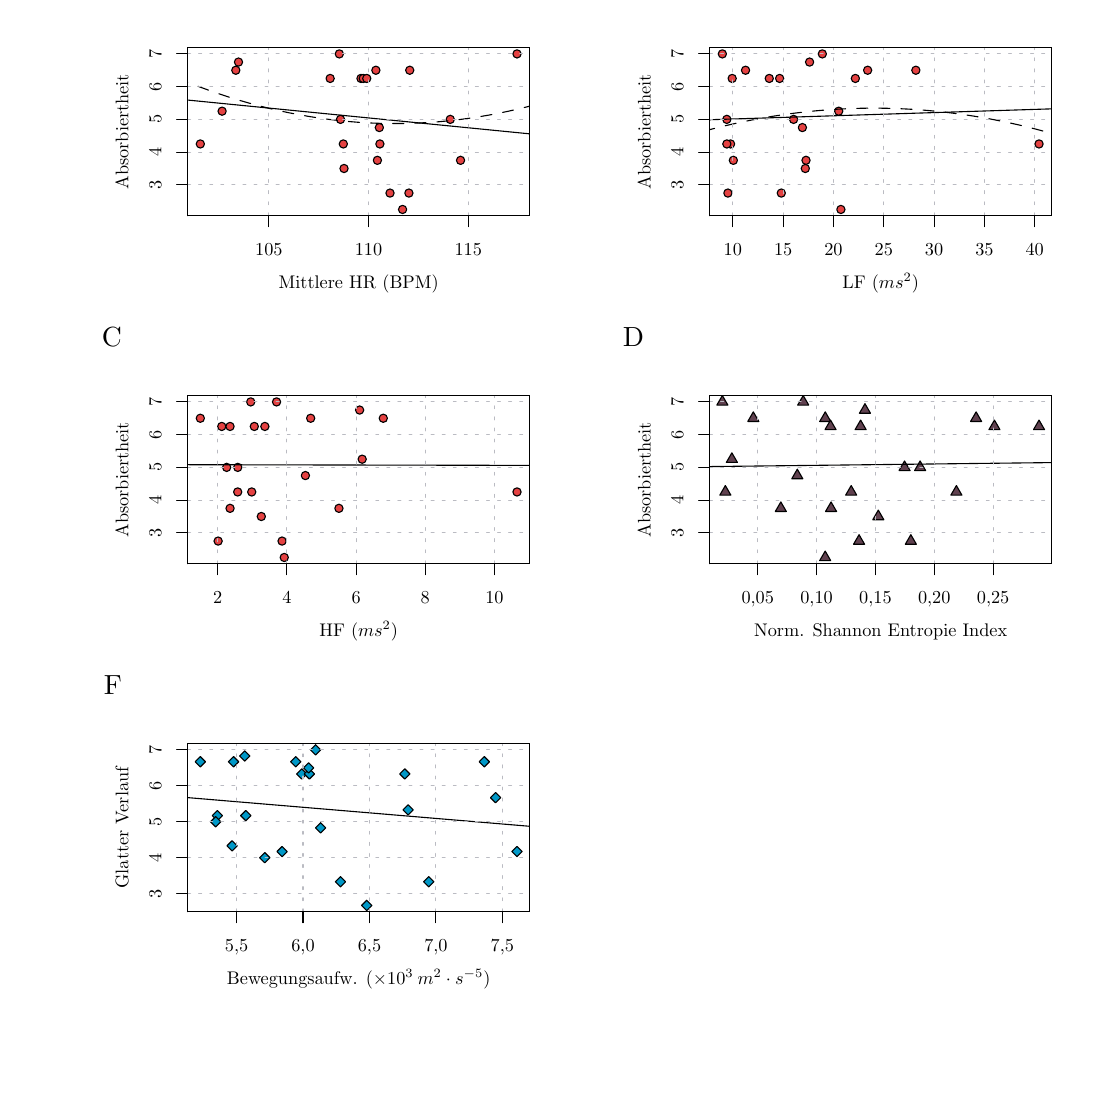
\begin{tikzpicture}[x=1pt,y=1pt]
\definecolor{fillColor}{RGB}{255,255,255}
\path[use as bounding box,fill=fillColor,fill opacity=0.00] (0,0) rectangle (377.25,377.25);
\begin{scope}
\path[clip] ( 57.82,309.32) rectangle (181.40,370.02);
\definecolor{drawColor}{RGB}{0,0,0}
\definecolor{fillColor}{RGB}{229,66,66}

\path[draw=drawColor,line width= 0.4pt,line join=round,line cap=round,fill=fillColor] (135.47,311.56) circle (  1.49);

\path[draw=drawColor,line width= 0.4pt,line join=round,line cap=round,fill=fillColor] (137.75,317.48) circle (  1.49);

\path[draw=drawColor,line width= 0.4pt,line join=round,line cap=round,fill=fillColor] (114.06,335.23) circle (  1.49);

\path[draw=drawColor,line width= 0.4pt,line join=round,line cap=round,fill=fillColor] (109.30,358.90) circle (  1.49);

\path[draw=drawColor,line width= 0.4pt,line join=round,line cap=round,fill=fillColor] (130.93,317.48) circle (  1.49);

\path[draw=drawColor,line width= 0.4pt,line join=round,line cap=round,fill=fillColor] (127.27,335.23) circle (  1.49);

\path[draw=drawColor,line width= 0.4pt,line join=round,line cap=round,fill=fillColor] (120.44,358.90) circle (  1.49);

\path[draw=drawColor,line width= 0.4pt,line join=round,line cap=round,fill=fillColor] (121.26,358.90) circle (  1.49);

\path[draw=drawColor,line width= 0.4pt,line join=round,line cap=round,fill=fillColor] (156.42,329.31) circle (  1.49);

\path[draw=drawColor,line width= 0.4pt,line join=round,line cap=round,fill=fillColor] (152.70,344.11) circle (  1.49);

\path[draw=drawColor,line width= 0.4pt,line join=round,line cap=round,fill=fillColor] (138.06,361.86) circle (  1.49);

\path[draw=drawColor,line width= 0.4pt,line join=round,line cap=round,fill=fillColor] ( 62.39,335.23) circle (  1.49);

\path[draw=drawColor,line width= 0.4pt,line join=round,line cap=round,fill=fillColor] ( 70.26,347.07) circle (  1.49);

\path[draw=drawColor,line width= 0.4pt,line join=round,line cap=round,fill=fillColor] ( 75.21,361.86) circle (  1.49);

\path[draw=drawColor,line width= 0.4pt,line join=round,line cap=round,fill=fillColor] ( 76.18,364.82) circle (  1.49);

\path[draw=drawColor,line width= 0.4pt,line join=round,line cap=round,fill=fillColor] (126.37,329.31) circle (  1.49);

\path[draw=drawColor,line width= 0.4pt,line join=round,line cap=round,fill=fillColor] (127.07,341.15) circle (  1.49);

\path[draw=drawColor,line width= 0.4pt,line join=round,line cap=round,fill=fillColor] (125.82,361.86) circle (  1.49);

\path[draw=drawColor,line width= 0.4pt,line join=round,line cap=round,fill=fillColor] (176.82,367.77) circle (  1.49);

\path[draw=drawColor,line width= 0.4pt,line join=round,line cap=round,fill=fillColor] (114.31,326.36) circle (  1.49);

\path[draw=drawColor,line width= 0.4pt,line join=round,line cap=round,fill=fillColor] (113.04,344.11) circle (  1.49);

\path[draw=drawColor,line width= 0.4pt,line join=round,line cap=round,fill=fillColor] (112.62,367.77) circle (  1.49);

\path[draw=drawColor,line width= 0.4pt,line join=round,line cap=round,fill=fillColor] (122.52,358.90) circle (  1.49);
\end{scope}
\begin{scope}
\path[clip] (  0.00,  0.00) rectangle (377.25,377.25);
\definecolor{drawColor}{RGB}{0,0,0}

\path[draw=drawColor,line width= 0.4pt,line join=round,line cap=round] ( 87.14,309.32) -- (159.21,309.32);

\path[draw=drawColor,line width= 0.4pt,line join=round,line cap=round] ( 87.14,309.32) -- ( 87.14,305.36);

\path[draw=drawColor,line width= 0.4pt,line join=round,line cap=round] (123.17,309.32) -- (123.17,305.36);

\path[draw=drawColor,line width= 0.4pt,line join=round,line cap=round] (159.21,309.32) -- (159.21,305.36);

\node[text=drawColor,anchor=base,inner sep=0pt, outer sep=0pt, scale=  0.66] at ( 87.14,295.06) {105};

\node[text=drawColor,anchor=base,inner sep=0pt, outer sep=0pt, scale=  0.66] at (123.17,295.06) {110};

\node[text=drawColor,anchor=base,inner sep=0pt, outer sep=0pt, scale=  0.66] at (159.21,295.06) {115};

\path[draw=drawColor,line width= 0.4pt,line join=round,line cap=round] ( 57.82,320.44) -- ( 57.82,367.77);

\path[draw=drawColor,line width= 0.4pt,line join=round,line cap=round] ( 57.82,320.44) -- ( 53.86,320.44);

\path[draw=drawColor,line width= 0.4pt,line join=round,line cap=round] ( 57.82,332.27) -- ( 53.86,332.27);

\path[draw=drawColor,line width= 0.4pt,line join=round,line cap=round] ( 57.82,344.11) -- ( 53.86,344.11);

\path[draw=drawColor,line width= 0.4pt,line join=round,line cap=round] ( 57.82,355.94) -- ( 53.86,355.94);

\path[draw=drawColor,line width= 0.4pt,line join=round,line cap=round] ( 57.82,367.77) -- ( 53.86,367.77);

\node[text=drawColor,rotate= 90.00,anchor=base,inner sep=0pt, outer sep=0pt, scale=  0.66] at ( 48.31,320.44) {3};

\node[text=drawColor,rotate= 90.00,anchor=base,inner sep=0pt, outer sep=0pt, scale=  0.66] at ( 48.31,332.27) {4};

\node[text=drawColor,rotate= 90.00,anchor=base,inner sep=0pt, outer sep=0pt, scale=  0.66] at ( 48.31,344.11) {5};

\node[text=drawColor,rotate= 90.00,anchor=base,inner sep=0pt, outer sep=0pt, scale=  0.66] at ( 48.31,355.94) {6};

\node[text=drawColor,rotate= 90.00,anchor=base,inner sep=0pt, outer sep=0pt, scale=  0.66] at ( 48.31,367.77) {7};

\path[draw=drawColor,line width= 0.4pt,line join=round,line cap=round] ( 57.82,309.32) --
	(181.40,309.32) --
	(181.40,370.02) --
	( 57.82,370.02) --
	( 57.82,309.32);
\end{scope}
\begin{scope}
\path[clip] (  0.00,251.50) rectangle (188.62,377.25);
\definecolor{drawColor}{RGB}{0,0,0}

\node[text=drawColor,anchor=base,inner sep=0pt, outer sep=0pt, scale=  0.66] at (119.61,283.18) {Mittlere HR (BPM)};

\node[text=drawColor,rotate= 90.00,anchor=base,inner sep=0pt, outer sep=0pt, scale=  0.66] at ( 36.43,339.67) {Absorbiertheit};
\end{scope}
\begin{scope}
\path[clip] ( 57.82,309.32) rectangle (181.40,370.02);
\definecolor{drawColor}{RGB}{0,0,0}

\path[draw=drawColor,line width= 0.4pt,line join=round,line cap=round] ( 57.82,351.09) -- (181.40,338.88);

\path[draw=drawColor,line width= 0.4pt,dash pattern=on 4pt off 4pt ,line join=round,line cap=round] ( 18.57,377.25) --
	( 18.67,377.19) --
	( 22.27,375.04) --
	( 25.88,372.96) --
	( 29.48,370.94) --
	( 33.08,369.00) --
	( 36.69,367.12) --
	( 40.29,365.32) --
	( 43.89,363.58) --
	( 47.50,361.91) --
	( 51.10,360.31) --
	( 54.70,358.78) --
	( 58.31,357.32) --
	( 61.91,355.93) --
	( 65.51,354.61) --
	( 69.12,353.35) --
	( 72.72,352.17) --
	( 76.33,351.05) --
	( 79.93,350.01) --
	( 83.53,349.03) --
	( 87.14,348.12) --
	( 90.74,347.28) --
	( 94.34,346.51) --
	( 97.95,345.81) --
	(101.55,345.18) --
	(105.15,344.61) --
	(108.76,344.12) --
	(112.36,343.70) --
	(115.96,343.34) --
	(119.57,343.05) --
	(123.17,342.83) --
	(126.78,342.69) --
	(130.38,342.61) --
	(133.98,342.60) --
	(137.59,342.65) --
	(141.19,342.78) --
	(144.79,342.98) --
	(148.40,343.24) --
	(152.00,343.58) --
	(155.60,343.98) --
	(159.21,344.46) --
	(162.81,345.00) --
	(166.41,345.61) --
	(170.02,346.29) --
	(173.62,347.04) --
	(177.23,347.86) --
	(180.83,348.74) --
	(184.43,349.70) --
	(188.04,350.72) --
	(191.64,351.82) --
	(195.24,352.98);
\definecolor{drawColor}{RGB}{186,187,194}

\path[draw=drawColor,line width= 0.4pt,dash pattern=on 1pt off 3pt ,line join=round,line cap=round] ( 87.14,309.32) -- ( 87.14,370.02);

\path[draw=drawColor,line width= 0.4pt,dash pattern=on 1pt off 3pt ,line join=round,line cap=round] (123.17,309.32) -- (123.17,370.02);

\path[draw=drawColor,line width= 0.4pt,dash pattern=on 1pt off 3pt ,line join=round,line cap=round] (159.21,309.32) -- (159.21,370.02);

\path[draw=drawColor,line width= 0.4pt,dash pattern=on 1pt off 3pt ,line join=round,line cap=round] ( 57.82,320.44) -- (181.40,320.44);

\path[draw=drawColor,line width= 0.4pt,dash pattern=on 1pt off 3pt ,line join=round,line cap=round] ( 57.82,332.27) -- (181.40,332.27);

\path[draw=drawColor,line width= 0.4pt,dash pattern=on 1pt off 3pt ,line join=round,line cap=round] ( 57.82,344.11) -- (181.40,344.11);

\path[draw=drawColor,line width= 0.4pt,dash pattern=on 1pt off 3pt ,line join=round,line cap=round] ( 57.82,355.94) -- (181.40,355.94);

\path[draw=drawColor,line width= 0.4pt,dash pattern=on 1pt off 3pt ,line join=round,line cap=round] ( 57.82,367.77) -- (181.40,367.77);
\end{scope}
\begin{scope}
\path[clip] (  0.00,  0.00) rectangle (377.25,377.25);
\definecolor{drawColor}{RGB}{0,0,0}

\path[draw=drawColor,line width= 0.4pt,line join=round,line cap=round] ( 57.82,309.32) --
	(181.40,309.32) --
	(181.40,370.02) --
	( 57.82,370.02) --
	( 57.82,309.32);
\end{scope}
\begin{scope}
\path[clip] (246.44,309.32) rectangle (370.02,370.02);
\definecolor{drawColor}{RGB}{0,0,0}
\definecolor{fillColor}{RGB}{229,66,66}

\path[draw=drawColor,line width= 0.4pt,line join=round,line cap=round,fill=fillColor] (293.85,311.56) circle (  1.49);

\path[draw=drawColor,line width= 0.4pt,line join=round,line cap=round,fill=fillColor] (253.02,317.48) circle (  1.49);

\path[draw=drawColor,line width= 0.4pt,line join=round,line cap=round,fill=fillColor] (253.99,335.23) circle (  1.49);

\path[draw=drawColor,line width= 0.4pt,line join=round,line cap=round,fill=fillColor] (271.72,358.90) circle (  1.49);

\path[draw=drawColor,line width= 0.4pt,line join=round,line cap=round,fill=fillColor] (272.32,317.48) circle (  1.49);

\path[draw=drawColor,line width= 0.4pt,line join=round,line cap=round,fill=fillColor] (252.64,335.23) circle (  1.49);

\path[draw=drawColor,line width= 0.4pt,line join=round,line cap=round,fill=fillColor] (267.97,358.90) circle (  1.49);

\path[draw=drawColor,line width= 0.4pt,line join=round,line cap=round,fill=fillColor] (254.57,358.90) circle (  1.49);

\path[draw=drawColor,line width= 0.4pt,line join=round,line cap=round,fill=fillColor] (254.99,329.31) circle (  1.49);

\path[draw=drawColor,line width= 0.4pt,line join=round,line cap=round,fill=fillColor] (252.63,344.11) circle (  1.49);

\path[draw=drawColor,line width= 0.4pt,line join=round,line cap=round,fill=fillColor] (259.40,361.86) circle (  1.49);

\path[draw=drawColor,line width= 0.4pt,line join=round,line cap=round,fill=fillColor] (365.45,335.23) circle (  1.49);

\path[draw=drawColor,line width= 0.4pt,line join=round,line cap=round,fill=fillColor] (293.07,347.07) circle (  1.49);

\path[draw=drawColor,line width= 0.4pt,line join=round,line cap=round,fill=fillColor] (320.94,361.86) circle (  1.49);

\path[draw=drawColor,line width= 0.4pt,line join=round,line cap=round,fill=fillColor] (282.54,364.82) circle (  1.49);

\path[draw=drawColor,line width= 0.4pt,line join=round,line cap=round,fill=fillColor] (281.25,329.31) circle (  1.49);

\path[draw=drawColor,line width= 0.4pt,line join=round,line cap=round,fill=fillColor] (279.94,341.15) circle (  1.49);

\path[draw=drawColor,line width= 0.4pt,line join=round,line cap=round,fill=fillColor] (303.52,361.86) circle (  1.49);

\path[draw=drawColor,line width= 0.4pt,line join=round,line cap=round,fill=fillColor] (251.02,367.77) circle (  1.49);

\path[draw=drawColor,line width= 0.4pt,line join=round,line cap=round,fill=fillColor] (280.99,326.36) circle (  1.49);

\path[draw=drawColor,line width= 0.4pt,line join=round,line cap=round,fill=fillColor] (276.76,344.11) circle (  1.49);

\path[draw=drawColor,line width= 0.4pt,line join=round,line cap=round,fill=fillColor] (287.15,367.77) circle (  1.49);

\path[draw=drawColor,line width= 0.4pt,line join=round,line cap=round,fill=fillColor] (299.08,358.90) circle (  1.49);
\end{scope}
\begin{scope}
\path[clip] (  0.00,  0.00) rectangle (377.25,377.25);
\definecolor{drawColor}{RGB}{0,0,0}

\path[draw=drawColor,line width= 0.4pt,line join=round,line cap=round] (254.81,309.32) -- (363.89,309.32);

\path[draw=drawColor,line width= 0.4pt,line join=round,line cap=round] (254.81,309.32) -- (254.81,305.36);

\path[draw=drawColor,line width= 0.4pt,line join=round,line cap=round] (272.99,309.32) -- (272.99,305.36);

\path[draw=drawColor,line width= 0.4pt,line join=round,line cap=round] (291.17,309.32) -- (291.17,305.36);

\path[draw=drawColor,line width= 0.4pt,line join=round,line cap=round] (309.35,309.32) -- (309.35,305.36);

\path[draw=drawColor,line width= 0.4pt,line join=round,line cap=round] (327.53,309.32) -- (327.53,305.36);

\path[draw=drawColor,line width= 0.4pt,line join=round,line cap=round] (345.71,309.32) -- (345.71,305.36);

\path[draw=drawColor,line width= 0.4pt,line join=round,line cap=round] (363.89,309.32) -- (363.89,305.36);

\node[text=drawColor,anchor=base,inner sep=0pt, outer sep=0pt, scale=  0.66] at (254.81,295.06) {10};

\node[text=drawColor,anchor=base,inner sep=0pt, outer sep=0pt, scale=  0.66] at (272.99,295.06) {15};

\node[text=drawColor,anchor=base,inner sep=0pt, outer sep=0pt, scale=  0.66] at (291.17,295.06) {20};

\node[text=drawColor,anchor=base,inner sep=0pt, outer sep=0pt, scale=  0.66] at (309.35,295.06) {25};

\node[text=drawColor,anchor=base,inner sep=0pt, outer sep=0pt, scale=  0.66] at (327.53,295.06) {30};

\node[text=drawColor,anchor=base,inner sep=0pt, outer sep=0pt, scale=  0.66] at (345.71,295.06) {35};

\node[text=drawColor,anchor=base,inner sep=0pt, outer sep=0pt, scale=  0.66] at (363.89,295.06) {40};

\path[draw=drawColor,line width= 0.4pt,line join=round,line cap=round] (246.44,320.44) -- (246.44,367.77);

\path[draw=drawColor,line width= 0.4pt,line join=round,line cap=round] (246.44,320.44) -- (242.48,320.44);

\path[draw=drawColor,line width= 0.4pt,line join=round,line cap=round] (246.44,332.27) -- (242.48,332.27);

\path[draw=drawColor,line width= 0.4pt,line join=round,line cap=round] (246.44,344.11) -- (242.48,344.11);

\path[draw=drawColor,line width= 0.4pt,line join=round,line cap=round] (246.44,355.94) -- (242.48,355.94);

\path[draw=drawColor,line width= 0.4pt,line join=round,line cap=round] (246.44,367.77) -- (242.48,367.77);

\node[text=drawColor,rotate= 90.00,anchor=base,inner sep=0pt, outer sep=0pt, scale=  0.66] at (236.94,320.44) {3};

\node[text=drawColor,rotate= 90.00,anchor=base,inner sep=0pt, outer sep=0pt, scale=  0.66] at (236.94,332.27) {4};

\node[text=drawColor,rotate= 90.00,anchor=base,inner sep=0pt, outer sep=0pt, scale=  0.66] at (236.94,344.11) {5};

\node[text=drawColor,rotate= 90.00,anchor=base,inner sep=0pt, outer sep=0pt, scale=  0.66] at (236.94,355.94) {6};

\node[text=drawColor,rotate= 90.00,anchor=base,inner sep=0pt, outer sep=0pt, scale=  0.66] at (236.94,367.77) {7};

\path[draw=drawColor,line width= 0.4pt,line join=round,line cap=round] (246.44,309.32) --
	(370.02,309.32) --
	(370.02,370.02) --
	(246.44,370.02) --
	(246.44,309.32);
\end{scope}
\begin{scope}
\path[clip] (188.62,251.50) rectangle (377.25,377.25);
\definecolor{drawColor}{RGB}{0,0,0}

\node[text=drawColor,anchor=base,inner sep=0pt, outer sep=0pt, scale=  0.66] at (308.23,283.18) {LF ($ms^2$)};

\node[text=drawColor,rotate= 90.00,anchor=base,inner sep=0pt, outer sep=0pt, scale=  0.66] at (225.06,339.67) {Absorbiertheit};
\end{scope}
\begin{scope}
\path[clip] (246.44,309.32) rectangle (370.02,370.02);
\definecolor{drawColor}{RGB}{0,0,0}

\path[draw=drawColor,line width= 0.4pt,line join=round,line cap=round] (246.44,343.98) -- (370.02,347.91);

\path[draw=drawColor,line width= 0.4pt,dash pattern=on 4pt off 4pt ,line join=round,line cap=round] (236.63,337.61) --
	(238.45,338.16) --
	(240.27,338.69) --
	(242.08,339.21) --
	(243.90,339.72) --
	(245.72,340.21) --
	(247.54,340.68) --
	(249.36,341.14) --
	(251.17,341.59) --
	(252.99,342.02) --
	(254.81,342.44) --
	(256.63,342.84) --
	(258.45,343.22) --
	(260.26,343.60) --
	(262.08,343.96) --
	(263.90,344.30) --
	(265.72,344.63) --
	(267.54,344.94) --
	(269.35,345.24) --
	(271.17,345.53) --
	(272.99,345.80) --
	(274.81,346.05) --
	(276.63,346.29) --
	(278.44,346.52) --
	(280.26,346.73) --
	(282.08,346.93) --
	(283.90,347.11) --
	(285.72,347.28) --
	(287.53,347.43) --
	(289.35,347.57) --
	(291.17,347.70) --
	(292.99,347.81) --
	(294.81,347.90) --
	(296.62,347.98) --
	(298.44,348.05) --
	(300.26,348.10) --
	(302.08,348.14) --
	(303.90,348.16) --
	(305.71,348.17) --
	(307.53,348.16) --
	(309.35,348.14) --
	(311.17,348.10) --
	(312.99,348.05) --
	(314.80,347.98) --
	(316.62,347.90) --
	(318.44,347.81) --
	(320.26,347.70) --
	(322.08,347.57) --
	(323.89,347.44) --
	(325.71,347.28) --
	(327.53,347.11) --
	(329.35,346.93) --
	(331.17,346.74) --
	(332.98,346.52) --
	(334.80,346.30) --
	(336.62,346.06) --
	(338.44,345.80) --
	(340.26,345.53) --
	(342.07,345.25) --
	(343.89,344.95) --
	(345.71,344.63) --
	(347.53,344.30) --
	(349.35,343.96) --
	(351.16,343.60) --
	(352.98,343.23) --
	(354.80,342.84) --
	(356.62,342.44) --
	(358.44,342.03) --
	(360.25,341.59) --
	(362.07,341.15) --
	(363.89,340.69) --
	(365.71,340.21) --
	(367.53,339.73) --
	(369.34,339.22) --
	(371.16,338.70) --
	(372.98,338.17) --
	(374.80,337.62) --
	(376.61,337.06) --
	(377.25,336.86);
\definecolor{drawColor}{RGB}{186,187,194}

\path[draw=drawColor,line width= 0.4pt,dash pattern=on 1pt off 3pt ,line join=round,line cap=round] (254.81,309.32) -- (254.81,370.02);

\path[draw=drawColor,line width= 0.4pt,dash pattern=on 1pt off 3pt ,line join=round,line cap=round] (272.99,309.32) -- (272.99,370.02);

\path[draw=drawColor,line width= 0.4pt,dash pattern=on 1pt off 3pt ,line join=round,line cap=round] (291.17,309.32) -- (291.17,370.02);

\path[draw=drawColor,line width= 0.4pt,dash pattern=on 1pt off 3pt ,line join=round,line cap=round] (309.35,309.32) -- (309.35,370.02);

\path[draw=drawColor,line width= 0.4pt,dash pattern=on 1pt off 3pt ,line join=round,line cap=round] (327.53,309.32) -- (327.53,370.02);

\path[draw=drawColor,line width= 0.4pt,dash pattern=on 1pt off 3pt ,line join=round,line cap=round] (345.71,309.32) -- (345.71,370.02);

\path[draw=drawColor,line width= 0.4pt,dash pattern=on 1pt off 3pt ,line join=round,line cap=round] (363.89,309.32) -- (363.89,370.02);

\path[draw=drawColor,line width= 0.4pt,dash pattern=on 1pt off 3pt ,line join=round,line cap=round] (246.44,320.44) -- (370.02,320.44);

\path[draw=drawColor,line width= 0.4pt,dash pattern=on 1pt off 3pt ,line join=round,line cap=round] (246.44,332.27) -- (370.02,332.27);

\path[draw=drawColor,line width= 0.4pt,dash pattern=on 1pt off 3pt ,line join=round,line cap=round] (246.44,344.11) -- (370.02,344.11);

\path[draw=drawColor,line width= 0.4pt,dash pattern=on 1pt off 3pt ,line join=round,line cap=round] (246.44,355.94) -- (370.02,355.94);

\path[draw=drawColor,line width= 0.4pt,dash pattern=on 1pt off 3pt ,line join=round,line cap=round] (246.44,367.77) -- (370.02,367.77);
\end{scope}
\begin{scope}
\path[clip] (  0.00,  0.00) rectangle (377.25,377.25);
\definecolor{drawColor}{RGB}{0,0,0}

\path[draw=drawColor,line width= 0.4pt,line join=round,line cap=round] (246.44,309.32) --
	(370.02,309.32) --
	(370.02,370.02) --
	(246.44,370.02) --
	(246.44,309.32);
\end{scope}
\begin{scope}
\path[clip] ( 57.82,183.57) rectangle (181.40,244.27);
\definecolor{drawColor}{RGB}{0,0,0}
\definecolor{fillColor}{RGB}{229,66,66}

\path[draw=drawColor,line width= 0.4pt,line join=round,line cap=round,fill=fillColor] ( 92.71,185.81) circle (  1.49);

\path[draw=drawColor,line width= 0.4pt,line join=round,line cap=round,fill=fillColor] ( 68.82,191.73) circle (  1.49);

\path[draw=drawColor,line width= 0.4pt,line join=round,line cap=round,fill=fillColor] ( 80.96,209.48) circle (  1.49);

\path[draw=drawColor,line width= 0.4pt,line join=round,line cap=round,fill=fillColor] ( 85.71,233.15) circle (  1.49);

\path[draw=drawColor,line width= 0.4pt,line join=round,line cap=round,fill=fillColor] ( 91.92,191.73) circle (  1.49);

\path[draw=drawColor,line width= 0.4pt,line join=round,line cap=round,fill=fillColor] ( 75.89,209.48) circle (  1.49);

\path[draw=drawColor,line width= 0.4pt,line join=round,line cap=round,fill=fillColor] ( 81.89,233.15) circle (  1.49);

\path[draw=drawColor,line width= 0.4pt,line join=round,line cap=round,fill=fillColor] ( 70.13,233.15) circle (  1.49);

\path[draw=drawColor,line width= 0.4pt,line join=round,line cap=round,fill=fillColor] ( 73.13,203.56) circle (  1.49);

\path[draw=drawColor,line width= 0.4pt,line join=round,line cap=round,fill=fillColor] ( 75.91,218.36) circle (  1.49);

\path[draw=drawColor,line width= 0.4pt,line join=round,line cap=round,fill=fillColor] ( 62.39,236.11) circle (  1.49);

\path[draw=drawColor,line width= 0.4pt,line join=round,line cap=round,fill=fillColor] (176.82,209.48) circle (  1.49);

\path[draw=drawColor,line width= 0.4pt,line join=round,line cap=round,fill=fillColor] (120.87,221.32) circle (  1.49);

\path[draw=drawColor,line width= 0.4pt,line join=round,line cap=round,fill=fillColor] (128.50,236.11) circle (  1.49);

\path[draw=drawColor,line width= 0.4pt,line join=round,line cap=round,fill=fillColor] (119.95,239.07) circle (  1.49);

\path[draw=drawColor,line width= 0.4pt,line join=round,line cap=round,fill=fillColor] (112.47,203.56) circle (  1.49);

\path[draw=drawColor,line width= 0.4pt,line join=round,line cap=round,fill=fillColor] (100.35,215.40) circle (  1.49);

\path[draw=drawColor,line width= 0.4pt,line join=round,line cap=round,fill=fillColor] (102.26,236.11) circle (  1.49);

\path[draw=drawColor,line width= 0.4pt,line join=round,line cap=round,fill=fillColor] ( 89.93,242.02) circle (  1.49);

\path[draw=drawColor,line width= 0.4pt,line join=round,line cap=round,fill=fillColor] ( 84.42,200.61) circle (  1.49);

\path[draw=drawColor,line width= 0.4pt,line join=round,line cap=round,fill=fillColor] ( 71.91,218.36) circle (  1.49);

\path[draw=drawColor,line width= 0.4pt,line join=round,line cap=round,fill=fillColor] ( 80.60,242.02) circle (  1.49);

\path[draw=drawColor,line width= 0.4pt,line join=round,line cap=round,fill=fillColor] ( 73.12,233.15) circle (  1.49);
\end{scope}
\begin{scope}
\path[clip] (  0.00,  0.00) rectangle (377.25,377.25);
\definecolor{drawColor}{RGB}{0,0,0}

\path[draw=drawColor,line width= 0.4pt,line join=round,line cap=round] ( 68.68,183.57) -- (168.67,183.57);

\path[draw=drawColor,line width= 0.4pt,line join=round,line cap=round] ( 68.68,183.57) -- ( 68.68,179.61);

\path[draw=drawColor,line width= 0.4pt,line join=round,line cap=round] ( 93.68,183.57) -- ( 93.68,179.61);

\path[draw=drawColor,line width= 0.4pt,line join=round,line cap=round] (118.67,183.57) -- (118.67,179.61);

\path[draw=drawColor,line width= 0.4pt,line join=round,line cap=round] (143.67,183.57) -- (143.67,179.61);

\path[draw=drawColor,line width= 0.4pt,line join=round,line cap=round] (168.67,183.57) -- (168.67,179.61);

\node[text=drawColor,anchor=base,inner sep=0pt, outer sep=0pt, scale=  0.66] at ( 68.68,169.31) {2};

\node[text=drawColor,anchor=base,inner sep=0pt, outer sep=0pt, scale=  0.66] at ( 93.68,169.31) {4};

\node[text=drawColor,anchor=base,inner sep=0pt, outer sep=0pt, scale=  0.66] at (118.67,169.31) {6};

\node[text=drawColor,anchor=base,inner sep=0pt, outer sep=0pt, scale=  0.66] at (143.67,169.31) {8};

\node[text=drawColor,anchor=base,inner sep=0pt, outer sep=0pt, scale=  0.66] at (168.67,169.31) {10};

\path[draw=drawColor,line width= 0.4pt,line join=round,line cap=round] ( 57.82,194.69) -- ( 57.82,242.02);

\path[draw=drawColor,line width= 0.4pt,line join=round,line cap=round] ( 57.82,194.69) -- ( 53.86,194.69);

\path[draw=drawColor,line width= 0.4pt,line join=round,line cap=round] ( 57.82,206.52) -- ( 53.86,206.52);

\path[draw=drawColor,line width= 0.4pt,line join=round,line cap=round] ( 57.82,218.36) -- ( 53.86,218.36);

\path[draw=drawColor,line width= 0.4pt,line join=round,line cap=round] ( 57.82,230.19) -- ( 53.86,230.19);

\path[draw=drawColor,line width= 0.4pt,line join=round,line cap=round] ( 57.82,242.02) -- ( 53.86,242.02);

\node[text=drawColor,rotate= 90.00,anchor=base,inner sep=0pt, outer sep=0pt, scale=  0.66] at ( 48.31,194.69) {3};

\node[text=drawColor,rotate= 90.00,anchor=base,inner sep=0pt, outer sep=0pt, scale=  0.66] at ( 48.31,206.52) {4};

\node[text=drawColor,rotate= 90.00,anchor=base,inner sep=0pt, outer sep=0pt, scale=  0.66] at ( 48.31,218.36) {5};

\node[text=drawColor,rotate= 90.00,anchor=base,inner sep=0pt, outer sep=0pt, scale=  0.66] at ( 48.31,230.19) {6};

\node[text=drawColor,rotate= 90.00,anchor=base,inner sep=0pt, outer sep=0pt, scale=  0.66] at ( 48.31,242.02) {7};

\path[draw=drawColor,line width= 0.4pt,line join=round,line cap=round] ( 57.82,183.57) --
	(181.40,183.57) --
	(181.40,244.27) --
	( 57.82,244.27) --
	( 57.82,183.57);
\end{scope}
\begin{scope}
\path[clip] (  0.00,125.75) rectangle (188.62,251.50);
\definecolor{drawColor}{RGB}{0,0,0}

\node[text=drawColor,anchor=base,inner sep=0pt, outer sep=0pt, scale=  0.66] at (119.61,157.43) {HF ($ms^2$)};

\node[text=drawColor,rotate= 90.00,anchor=base,inner sep=0pt, outer sep=0pt, scale=  0.66] at ( 36.43,213.92) {Absorbiertheit};
\end{scope}
\begin{scope}
\path[clip] ( 57.82,183.57) rectangle (181.40,244.27);
\definecolor{drawColor}{RGB}{0,0,0}

\path[draw=drawColor,line width= 0.4pt,line join=round,line cap=round] ( 57.82,219.33) -- (181.40,219.08);
\definecolor{drawColor}{RGB}{186,187,194}

\path[draw=drawColor,line width= 0.4pt,dash pattern=on 1pt off 3pt ,line join=round,line cap=round] ( 68.68,183.57) -- ( 68.68,244.27);

\path[draw=drawColor,line width= 0.4pt,dash pattern=on 1pt off 3pt ,line join=round,line cap=round] ( 93.68,183.57) -- ( 93.68,244.27);

\path[draw=drawColor,line width= 0.4pt,dash pattern=on 1pt off 3pt ,line join=round,line cap=round] (118.67,183.57) -- (118.67,244.27);

\path[draw=drawColor,line width= 0.4pt,dash pattern=on 1pt off 3pt ,line join=round,line cap=round] (143.67,183.57) -- (143.67,244.27);

\path[draw=drawColor,line width= 0.4pt,dash pattern=on 1pt off 3pt ,line join=round,line cap=round] (168.67,183.57) -- (168.67,244.27);

\path[draw=drawColor,line width= 0.4pt,dash pattern=on 1pt off 3pt ,line join=round,line cap=round] ( 57.82,194.69) -- (181.40,194.69);

\path[draw=drawColor,line width= 0.4pt,dash pattern=on 1pt off 3pt ,line join=round,line cap=round] ( 57.82,206.52) -- (181.40,206.52);

\path[draw=drawColor,line width= 0.4pt,dash pattern=on 1pt off 3pt ,line join=round,line cap=round] ( 57.82,218.36) -- (181.40,218.36);

\path[draw=drawColor,line width= 0.4pt,dash pattern=on 1pt off 3pt ,line join=round,line cap=round] ( 57.82,230.19) -- (181.40,230.19);

\path[draw=drawColor,line width= 0.4pt,dash pattern=on 1pt off 3pt ,line join=round,line cap=round] ( 57.82,242.02) -- (181.40,242.02);
\end{scope}
\begin{scope}
\path[clip] (  0.00,  0.00) rectangle (377.25,377.25);
\definecolor{drawColor}{RGB}{0,0,0}

\path[draw=drawColor,line width= 0.4pt,line join=round,line cap=round] ( 57.82,183.57) --
	(181.40,183.57) --
	(181.40,244.27) --
	( 57.82,244.27) --
	( 57.82,183.57);

\node[text=drawColor,anchor=base east,inner sep=0pt, outer sep=0pt, scale=  1.00] at ( 34.06,262.13) {C};
\end{scope}
\begin{scope}
\path[clip] (246.44,183.57) rectangle (370.02,244.27);
\definecolor{drawColor}{RGB}{0,0,0}
\definecolor{fillColor}{RGB}{96,65,79}

\path[draw=drawColor,line width= 0.4pt,line join=round,line cap=round,fill=fillColor] (288.18,188.12) --
	(290.18,184.66) --
	(286.18,184.66) --
	cycle;

\path[draw=drawColor,line width= 0.4pt,line join=round,line cap=round,fill=fillColor] (319.13,194.04) --
	(321.13,190.58) --
	(317.13,190.58) --
	cycle;

\path[draw=drawColor,line width= 0.4pt,line join=round,line cap=round,fill=fillColor] (335.59,211.79) --
	(337.59,208.33) --
	(333.59,208.33) --
	cycle;

\path[draw=drawColor,line width= 0.4pt,line join=round,line cap=round,fill=fillColor] (300.98,235.46) --
	(302.98,231.99) --
	(298.98,231.99) --
	cycle;

\path[draw=drawColor,line width= 0.4pt,line join=round,line cap=round,fill=fillColor] (300.42,194.04) --
	(302.42,190.58) --
	(298.42,190.58) --
	cycle;

\path[draw=drawColor,line width= 0.4pt,line join=round,line cap=round,fill=fillColor] (297.57,211.79) --
	(299.57,208.33) --
	(295.57,208.33) --
	cycle;

\path[draw=drawColor,line width= 0.4pt,line join=round,line cap=round,fill=fillColor] (365.45,235.46) --
	(367.45,231.99) --
	(363.45,231.99) --
	cycle;

\path[draw=drawColor,line width= 0.4pt,line join=round,line cap=round,fill=fillColor] (349.34,235.46) --
	(351.34,231.99) --
	(347.34,231.99) --
	cycle;

\path[draw=drawColor,line width= 0.4pt,line join=round,line cap=round,fill=fillColor] (290.30,205.87) --
	(292.30,202.41) --
	(288.30,202.41) --
	cycle;

\path[draw=drawColor,line width= 0.4pt,line join=round,line cap=round,fill=fillColor] (316.85,220.67) --
	(318.85,217.20) --
	(314.85,217.20) --
	cycle;

\path[draw=drawColor,line width= 0.4pt,line join=round,line cap=round,fill=fillColor] (342.71,238.42) --
	(344.71,234.95) --
	(340.71,234.95) --
	cycle;

\path[draw=drawColor,line width= 0.4pt,line join=round,line cap=round,fill=fillColor] (252.10,211.79) --
	(254.10,208.33) --
	(250.10,208.33) --
	cycle;

\path[draw=drawColor,line width= 0.4pt,line join=round,line cap=round,fill=fillColor] (254.46,223.62) --
	(256.46,220.16) --
	(252.46,220.16) --
	cycle;

\path[draw=drawColor,line width= 0.4pt,line join=round,line cap=round,fill=fillColor] (262.21,238.42) --
	(264.21,234.95) --
	(260.21,234.95) --
	cycle;

\path[draw=drawColor,line width= 0.4pt,line join=round,line cap=round,fill=fillColor] (302.55,241.38) --
	(304.55,237.91) --
	(300.55,237.91) --
	cycle;

\path[draw=drawColor,line width= 0.4pt,line join=round,line cap=round,fill=fillColor] (272.15,205.87) --
	(274.15,202.41) --
	(270.15,202.41) --
	cycle;

\path[draw=drawColor,line width= 0.4pt,line join=round,line cap=round,fill=fillColor] (278.10,217.71) --
	(280.10,214.24) --
	(276.10,214.24) --
	cycle;

\path[draw=drawColor,line width= 0.4pt,line join=round,line cap=round,fill=fillColor] (288.20,238.42) --
	(290.20,234.95) --
	(286.20,234.95) --
	cycle;

\path[draw=drawColor,line width= 0.4pt,line join=round,line cap=round,fill=fillColor] (251.02,244.33) --
	(253.02,240.87) --
	(249.02,240.87) --
	cycle;

\path[draw=drawColor,line width= 0.4pt,line join=round,line cap=round,fill=fillColor] (307.37,202.92) --
	(309.37,199.45) --
	(305.37,199.45) --
	cycle;

\path[draw=drawColor,line width= 0.4pt,line join=round,line cap=round,fill=fillColor] (322.48,220.67) --
	(324.48,217.20) --
	(320.48,217.20) --
	cycle;

\path[draw=drawColor,line width= 0.4pt,line join=round,line cap=round,fill=fillColor] (280.24,244.33) --
	(282.24,240.87) --
	(278.24,240.87) --
	cycle;

\path[draw=drawColor,line width= 0.4pt,line join=round,line cap=round,fill=fillColor] (290.11,235.46) --
	(292.11,231.99) --
	(288.11,231.99) --
	cycle;
\end{scope}
\begin{scope}
\path[clip] (  0.00,  0.00) rectangle (377.25,377.25);
\definecolor{drawColor}{RGB}{0,0,0}

\path[draw=drawColor,line width= 0.4pt,line join=round,line cap=round] (263.81,183.57) -- (348.87,183.57);

\path[draw=drawColor,line width= 0.4pt,line join=round,line cap=round] (263.81,183.57) -- (263.81,179.61);

\path[draw=drawColor,line width= 0.4pt,line join=round,line cap=round] (285.07,183.57) -- (285.07,179.61);

\path[draw=drawColor,line width= 0.4pt,line join=round,line cap=round] (306.34,183.57) -- (306.34,179.61);

\path[draw=drawColor,line width= 0.4pt,line join=round,line cap=round] (327.60,183.57) -- (327.60,179.61);

\path[draw=drawColor,line width= 0.4pt,line join=round,line cap=round] (348.87,183.57) -- (348.87,179.61);

\node[text=drawColor,anchor=base,inner sep=0pt, outer sep=0pt, scale=  0.66] at (263.81,169.31) {0,05};

\node[text=drawColor,anchor=base,inner sep=0pt, outer sep=0pt, scale=  0.66] at (285.07,169.31) {0,10};

\node[text=drawColor,anchor=base,inner sep=0pt, outer sep=0pt, scale=  0.66] at (306.34,169.31) {0,15};

\node[text=drawColor,anchor=base,inner sep=0pt, outer sep=0pt, scale=  0.66] at (327.60,169.31) {0,20};

\node[text=drawColor,anchor=base,inner sep=0pt, outer sep=0pt, scale=  0.66] at (348.87,169.31) {0,25};

\path[draw=drawColor,line width= 0.4pt,line join=round,line cap=round] (246.44,194.69) -- (246.44,242.02);

\path[draw=drawColor,line width= 0.4pt,line join=round,line cap=round] (246.44,194.69) -- (242.48,194.69);

\path[draw=drawColor,line width= 0.4pt,line join=round,line cap=round] (246.44,206.52) -- (242.48,206.52);

\path[draw=drawColor,line width= 0.4pt,line join=round,line cap=round] (246.44,218.36) -- (242.48,218.36);

\path[draw=drawColor,line width= 0.4pt,line join=round,line cap=round] (246.44,230.19) -- (242.48,230.19);

\path[draw=drawColor,line width= 0.4pt,line join=round,line cap=round] (246.44,242.02) -- (242.48,242.02);

\node[text=drawColor,rotate= 90.00,anchor=base,inner sep=0pt, outer sep=0pt, scale=  0.66] at (236.94,194.69) {3};

\node[text=drawColor,rotate= 90.00,anchor=base,inner sep=0pt, outer sep=0pt, scale=  0.66] at (236.94,206.52) {4};

\node[text=drawColor,rotate= 90.00,anchor=base,inner sep=0pt, outer sep=0pt, scale=  0.66] at (236.94,218.36) {5};

\node[text=drawColor,rotate= 90.00,anchor=base,inner sep=0pt, outer sep=0pt, scale=  0.66] at (236.94,230.19) {6};

\node[text=drawColor,rotate= 90.00,anchor=base,inner sep=0pt, outer sep=0pt, scale=  0.66] at (236.94,242.02) {7};

\path[draw=drawColor,line width= 0.4pt,line join=round,line cap=round] (246.44,183.57) --
	(370.02,183.57) --
	(370.02,244.27) --
	(246.44,244.27) --
	(246.44,183.57);
\end{scope}
\begin{scope}
\path[clip] (188.62,125.75) rectangle (377.25,251.50);
\definecolor{drawColor}{RGB}{0,0,0}

\node[text=drawColor,anchor=base,inner sep=0pt, outer sep=0pt, scale=  0.66] at (308.23,157.43) {Norm. Shannon Entropie Index};

\node[text=drawColor,rotate= 90.00,anchor=base,inner sep=0pt, outer sep=0pt, scale=  0.66] at (225.06,213.92) {Absorbiertheit};
\end{scope}
\begin{scope}
\path[clip] (246.44,183.57) rectangle (370.02,244.27);
\definecolor{drawColor}{RGB}{0,0,0}

\path[draw=drawColor,line width= 0.4pt,line join=round,line cap=round] (246.44,218.65) -- (370.02,220.09);
\definecolor{drawColor}{RGB}{186,187,194}

\path[draw=drawColor,line width= 0.4pt,dash pattern=on 1pt off 3pt ,line join=round,line cap=round] (263.81,183.57) -- (263.81,244.27);

\path[draw=drawColor,line width= 0.4pt,dash pattern=on 1pt off 3pt ,line join=round,line cap=round] (285.07,183.57) -- (285.07,244.27);

\path[draw=drawColor,line width= 0.4pt,dash pattern=on 1pt off 3pt ,line join=round,line cap=round] (306.34,183.57) -- (306.34,244.27);

\path[draw=drawColor,line width= 0.4pt,dash pattern=on 1pt off 3pt ,line join=round,line cap=round] (327.60,183.57) -- (327.60,244.27);

\path[draw=drawColor,line width= 0.4pt,dash pattern=on 1pt off 3pt ,line join=round,line cap=round] (348.87,183.57) -- (348.87,244.27);

\path[draw=drawColor,line width= 0.4pt,dash pattern=on 1pt off 3pt ,line join=round,line cap=round] (246.44,194.69) -- (370.02,194.69);

\path[draw=drawColor,line width= 0.4pt,dash pattern=on 1pt off 3pt ,line join=round,line cap=round] (246.44,206.52) -- (370.02,206.52);

\path[draw=drawColor,line width= 0.4pt,dash pattern=on 1pt off 3pt ,line join=round,line cap=round] (246.44,218.36) -- (370.02,218.36);

\path[draw=drawColor,line width= 0.4pt,dash pattern=on 1pt off 3pt ,line join=round,line cap=round] (246.44,230.19) -- (370.02,230.19);

\path[draw=drawColor,line width= 0.4pt,dash pattern=on 1pt off 3pt ,line join=round,line cap=round] (246.44,242.02) -- (370.02,242.02);
\end{scope}
\begin{scope}
\path[clip] (  0.00,  0.00) rectangle (377.25,377.25);
\definecolor{drawColor}{RGB}{0,0,0}

\path[draw=drawColor,line width= 0.4pt,line join=round,line cap=round] (246.44,183.57) --
	(370.02,183.57) --
	(370.02,244.27) --
	(246.44,244.27) --
	(246.44,183.57);

\node[text=drawColor,anchor=base east,inner sep=0pt, outer sep=0pt, scale=  1.00] at (222.68,262.13) {D};
\end{scope}
\begin{scope}
\path[clip] ( 57.82, 57.82) rectangle (181.40,118.52);
\definecolor{drawColor}{RGB}{0,0,0}
\definecolor{fillColor}{RGB}{0,152,199}

\path[draw=drawColor,line width= 0.4pt,line join=round,line cap=round,fill=fillColor] (122.51, 58.20) --
	(124.37, 60.06) --
	(122.51, 61.93) --
	(120.65, 60.06) --
	cycle;

\path[draw=drawColor,line width= 0.4pt,line join=round,line cap=round,fill=fillColor] (144.94, 66.77) --
	(146.80, 68.63) --
	(144.94, 70.49) --
	(143.08, 68.63) --
	cycle;

\path[draw=drawColor,line width= 0.4pt,line join=round,line cap=round,fill=fillColor] (137.49, 92.73) --
	(139.35, 94.60) --
	(137.49, 96.46) --
	(135.62, 94.60) --
	cycle;

\path[draw=drawColor,line width= 0.4pt,line join=round,line cap=round,fill=fillColor] (136.28,105.72) --
	(138.14,107.58) --
	(136.28,109.44) --
	(134.42,107.58) --
	cycle;

\path[draw=drawColor,line width= 0.4pt,line join=round,line cap=round,fill=fillColor] (113.02, 66.77) --
	(114.88, 68.63) --
	(113.02, 70.49) --
	(111.16, 68.63) --
	cycle;

\path[draw=drawColor,line width= 0.4pt,line join=round,line cap=round,fill=fillColor] (105.85, 86.24) --
	(107.71, 88.10) --
	(105.85, 89.97) --
	(103.99, 88.10) --
	cycle;

\path[draw=drawColor,line width= 0.4pt,line join=round,line cap=round,fill=fillColor] ( 99.05,105.72) --
	(100.91,107.58) --
	( 99.05,109.44) --
	( 97.18,107.58) --
	cycle;

\path[draw=drawColor,line width= 0.4pt,line join=round,line cap=round,fill=fillColor] (101.79,105.72) --
	(103.65,107.58) --
	(101.79,109.44) --
	( 99.93,107.58) --
	cycle;

\path[draw=drawColor,line width= 0.4pt,line join=round,line cap=round,fill=fillColor] (176.82, 77.68) --
	(178.68, 79.54) --
	(176.82, 81.40) --
	(174.96, 79.54) --
	cycle;

\path[draw=drawColor,line width= 0.4pt,line join=round,line cap=round,fill=fillColor] (169.07, 97.15) --
	(170.93, 99.01) --
	(169.07,100.87) --
	(167.21, 99.01) --
	cycle;

\path[draw=drawColor,line width= 0.4pt,line join=round,line cap=round,fill=fillColor] (165.01,110.13) --
	(166.87,111.99) --
	(165.01,113.85) --
	(163.15,111.99) --
	cycle;

\path[draw=drawColor,line width= 0.4pt,line join=round,line cap=round,fill=fillColor] ( 73.86, 79.75) --
	( 75.72, 81.61) --
	( 73.86, 83.47) --
	( 72.00, 81.61) --
	cycle;

\path[draw=drawColor,line width= 0.4pt,line join=round,line cap=round,fill=fillColor] ( 68.53, 90.66) --
	( 70.39, 92.52) --
	( 68.53, 94.38) --
	( 66.67, 92.52) --
	cycle;

\path[draw=drawColor,line width= 0.4pt,line join=round,line cap=round,fill=fillColor] ( 74.41,110.13) --
	( 76.27,111.99) --
	( 74.41,113.85) --
	( 72.54,111.99) --
	cycle;

\path[draw=drawColor,line width= 0.4pt,line join=round,line cap=round,fill=fillColor] ( 62.39,110.13) --
	( 64.25,111.99) --
	( 62.39,113.85) --
	( 60.53,111.99) --
	cycle;

\path[draw=drawColor,line width= 0.4pt,line join=round,line cap=round,fill=fillColor] ( 91.93, 77.68) --
	( 93.79, 79.54) --
	( 91.93, 81.40) --
	( 90.07, 79.54) --
	cycle;

\path[draw=drawColor,line width= 0.4pt,line join=round,line cap=round,fill=fillColor] ( 67.92, 88.45) --
	( 69.79, 90.31) --
	( 67.92, 92.17) --
	( 66.06, 90.31) --
	cycle;

\path[draw=drawColor,line width= 0.4pt,line join=round,line cap=round,fill=fillColor] ( 78.44,112.21) --
	( 80.30,114.07) --
	( 78.44,115.93) --
	( 76.58,114.07) --
	cycle;

\path[draw=drawColor,line width= 0.4pt,line join=round,line cap=round,fill=fillColor] ( 96.88,110.13) --
	( 98.74,111.99) --
	( 96.88,113.85) --
	( 95.02,111.99) --
	cycle;

\path[draw=drawColor,line width= 0.4pt,line join=round,line cap=round,fill=fillColor] ( 85.67, 75.47) --
	( 87.53, 77.33) --
	( 85.67, 79.19) --
	( 83.81, 77.33) --
	cycle;

\path[draw=drawColor,line width= 0.4pt,line join=round,line cap=round,fill=fillColor] ( 78.81, 90.66) --
	( 80.67, 92.52) --
	( 78.81, 94.38) --
	( 76.94, 92.52) --
	cycle;

\path[draw=drawColor,line width= 0.4pt,line join=round,line cap=round,fill=fillColor] (101.54,107.92) --
	(103.40,109.78) --
	(101.54,111.64) --
	( 99.68,109.78) --
	cycle;

\path[draw=drawColor,line width= 0.4pt,line join=round,line cap=round,fill=fillColor] (104.05,114.41) --
	(105.91,116.27) --
	(104.05,118.14) --
	(102.19,116.27) --
	cycle;
\end{scope}
\begin{scope}
\path[clip] (  0.00,  0.00) rectangle (377.25,377.25);
\definecolor{drawColor}{RGB}{0,0,0}

\path[draw=drawColor,line width= 0.4pt,line join=round,line cap=round] ( 75.49, 57.82) -- (171.54, 57.82);

\path[draw=drawColor,line width= 0.4pt,line join=round,line cap=round] ( 75.49, 57.82) -- ( 75.49, 53.86);

\path[draw=drawColor,line width= 0.4pt,line join=round,line cap=round] ( 99.50, 57.82) -- ( 99.50, 53.86);

\path[draw=drawColor,line width= 0.4pt,line join=round,line cap=round] (123.51, 57.82) -- (123.51, 53.86);

\path[draw=drawColor,line width= 0.4pt,line join=round,line cap=round] (147.52, 57.82) -- (147.52, 53.86);

\path[draw=drawColor,line width= 0.4pt,line join=round,line cap=round] (171.54, 57.82) -- (171.54, 53.86);

\node[text=drawColor,anchor=base,inner sep=0pt, outer sep=0pt, scale=  0.66] at ( 75.49, 43.56) {5,5};

\node[text=drawColor,anchor=base,inner sep=0pt, outer sep=0pt, scale=  0.66] at ( 99.50, 43.56) {6,0};

\node[text=drawColor,anchor=base,inner sep=0pt, outer sep=0pt, scale=  0.66] at (123.51, 43.56) {6,5};

\node[text=drawColor,anchor=base,inner sep=0pt, outer sep=0pt, scale=  0.66] at (147.52, 43.56) {7,0};

\node[text=drawColor,anchor=base,inner sep=0pt, outer sep=0pt, scale=  0.66] at (171.54, 43.56) {7,5};

\path[draw=drawColor,line width= 0.4pt,line join=round,line cap=round] ( 57.82, 64.35) -- ( 57.82,116.27);

\path[draw=drawColor,line width= 0.4pt,line join=round,line cap=round] ( 57.82, 64.35) -- ( 53.86, 64.35);

\path[draw=drawColor,line width= 0.4pt,line join=round,line cap=round] ( 57.82, 77.33) -- ( 53.86, 77.33);

\path[draw=drawColor,line width= 0.4pt,line join=round,line cap=round] ( 57.82, 90.31) -- ( 53.86, 90.31);

\path[draw=drawColor,line width= 0.4pt,line join=round,line cap=round] ( 57.82,103.29) -- ( 53.86,103.29);

\path[draw=drawColor,line width= 0.4pt,line join=round,line cap=round] ( 57.82,116.27) -- ( 53.86,116.27);

\node[text=drawColor,rotate= 90.00,anchor=base,inner sep=0pt, outer sep=0pt, scale=  0.66] at ( 48.31, 64.35) {3};

\node[text=drawColor,rotate= 90.00,anchor=base,inner sep=0pt, outer sep=0pt, scale=  0.66] at ( 48.31, 77.33) {4};

\node[text=drawColor,rotate= 90.00,anchor=base,inner sep=0pt, outer sep=0pt, scale=  0.66] at ( 48.31, 90.31) {5};

\node[text=drawColor,rotate= 90.00,anchor=base,inner sep=0pt, outer sep=0pt, scale=  0.66] at ( 48.31,103.29) {6};

\node[text=drawColor,rotate= 90.00,anchor=base,inner sep=0pt, outer sep=0pt, scale=  0.66] at ( 48.31,116.27) {7};

\path[draw=drawColor,line width= 0.4pt,line join=round,line cap=round] ( 57.82, 57.82) --
	(181.40, 57.82) --
	(181.40,118.52) --
	( 57.82,118.52) --
	( 57.82, 57.82);
\end{scope}
\begin{scope}
\path[clip] (  0.00,  0.00) rectangle (188.62,125.75);
\definecolor{drawColor}{RGB}{0,0,0}

\node[text=drawColor,anchor=base,inner sep=0pt, outer sep=0pt, scale=  0.66] at (119.61, 31.68) {Bewegungsaufw. ($\times 10^3 \: m^2 \cdot s^{-5}$)};

\node[text=drawColor,rotate= 90.00,anchor=base,inner sep=0pt, outer sep=0pt, scale=  0.66] at ( 36.43, 88.17) {Glatter Verlauf};
\end{scope}
\begin{scope}
\path[clip] ( 57.82, 57.82) rectangle (181.40,118.52);
\definecolor{drawColor}{RGB}{0,0,0}

\path[draw=drawColor,line width= 0.4pt,line join=round,line cap=round] ( 57.82, 99.03) -- (181.40, 88.67);
\definecolor{drawColor}{RGB}{186,187,194}

\path[draw=drawColor,line width= 0.4pt,dash pattern=on 1pt off 3pt ,line join=round,line cap=round] ( 75.49, 57.82) -- ( 75.49,118.52);

\path[draw=drawColor,line width= 0.4pt,dash pattern=on 1pt off 3pt ,line join=round,line cap=round] ( 99.50, 57.82) -- ( 99.50,118.52);

\path[draw=drawColor,line width= 0.4pt,dash pattern=on 1pt off 3pt ,line join=round,line cap=round] (123.51, 57.82) -- (123.51,118.52);

\path[draw=drawColor,line width= 0.4pt,dash pattern=on 1pt off 3pt ,line join=round,line cap=round] (147.52, 57.82) -- (147.52,118.52);

\path[draw=drawColor,line width= 0.4pt,dash pattern=on 1pt off 3pt ,line join=round,line cap=round] (171.54, 57.82) -- (171.54,118.52);

\path[draw=drawColor,line width= 0.4pt,dash pattern=on 1pt off 3pt ,line join=round,line cap=round] ( 57.82, 64.35) -- (181.40, 64.35);

\path[draw=drawColor,line width= 0.4pt,dash pattern=on 1pt off 3pt ,line join=round,line cap=round] ( 57.82, 77.33) -- (181.40, 77.33);

\path[draw=drawColor,line width= 0.4pt,dash pattern=on 1pt off 3pt ,line join=round,line cap=round] ( 57.82, 90.31) -- (181.40, 90.31);

\path[draw=drawColor,line width= 0.4pt,dash pattern=on 1pt off 3pt ,line join=round,line cap=round] ( 57.82,103.29) -- (181.40,103.29);

\path[draw=drawColor,line width= 0.4pt,dash pattern=on 1pt off 3pt ,line join=round,line cap=round] ( 57.82,116.27) -- (181.40,116.27);
\end{scope}
\begin{scope}
\path[clip] (  0.00,  0.00) rectangle (377.25,377.25);
\definecolor{drawColor}{RGB}{0,0,0}

\path[draw=drawColor,line width= 0.4pt,line join=round,line cap=round] ( 57.82, 57.82) --
	(181.40, 57.82) --
	(181.40,118.52) --
	( 57.82,118.52) --
	( 57.82, 57.82);

\node[text=drawColor,anchor=base east,inner sep=0pt, outer sep=0pt, scale=  1.00] at ( 34.06,136.38) {F};
\end{scope}
\end{tikzpicture}

% 	\caption[Beobachtungen der Fallstudie zum Flow-Erleben beim Gehen]{Beobachtungen der Fallstudie zum Flow-Erleben beim Gehen. (A) Absorbiertheit und mittlerer HR; (B) Absorbiertheit und LF; (C) Absorbiertheit und HF; (D) Absorbiertheit und mittlerer normalisierter Shannon Entropie Index; (F) Glatter Verlauf und mittlerer Bewegungsaufwand. Quelle: Eigene Darstellung \\ \hspace{\textwidth}\emph{Anmerkung}: Durchgezogene Linie stellt das bestmögliche liniare Modell dar. \\ \hspace{\textwidth}Gestrichelte Linie stellt ggf. das bestmögliche quardratische Modell dar.}
% 	\label{fig:B_2_regression}
% \end{figure}
%
% \begin{figure}
% 	% Created by tikzDevice version 0.10.1 on 2016-06-20 06:48:37
% !TEX encoding = UTF-8 Unicode
\begin{tikzpicture}[x=1pt,y=1pt]
\definecolor{fillColor}{RGB}{255,255,255}
\path[use as bounding box,fill=fillColor,fill opacity=0.00] (0,0) rectangle (377.25,377.25);
\begin{scope}
\path[clip] ( 57.82, 57.82) rectangle (370.02,370.02);
\definecolor{drawColor}{RGB}{0,0,0}
\definecolor{fillColor}{RGB}{229,66,66}

\path[draw=drawColor,line width= 0.4pt,line join=round,line cap=round,fill=fillColor] (205.43, 71.88) circle (  2.25);

\path[draw=drawColor,line width= 0.4pt,line join=round,line cap=round,fill=fillColor] (304.72,178.94) circle (  2.25);

\path[draw=drawColor,line width= 0.4pt,line join=round,line cap=round,fill=fillColor] (316.65, 72.11) circle (  2.25);

\path[draw=drawColor,line width= 0.4pt,line join=round,line cap=round,fill=fillColor] (128.05, 73.99) circle (  2.25);

\path[draw=drawColor,line width= 0.4pt,line join=round,line cap=round,fill=fillColor] (259.21,103.50) circle (  2.25);

\path[draw=drawColor,line width= 0.4pt,line join=round,line cap=round,fill=fillColor] (222.49,175.80) circle (  2.25);

\path[draw=drawColor,line width= 0.4pt,line join=round,line cap=round,fill=fillColor] (232.49,133.85) circle (  2.25);

\path[draw=drawColor,line width= 0.4pt,line join=round,line cap=round,fill=fillColor] (305.58, 70.95) circle (  2.25);

\path[draw=drawColor,line width= 0.4pt,line join=round,line cap=round,fill=fillColor] (358.46, 69.86) circle (  2.25);

\path[draw=drawColor,line width= 0.4pt,line join=round,line cap=round,fill=fillColor] (299.88,198.32) circle (  2.25);

\path[draw=drawColor,line width= 0.4pt,line join=round,line cap=round,fill=fillColor] (331.18,107.04) circle (  2.25);

\path[draw=drawColor,line width= 0.4pt,line join=round,line cap=round,fill=fillColor] (269.64, 98.16) circle (  2.25);

\path[draw=drawColor,line width= 0.4pt,line join=round,line cap=round,fill=fillColor] (269.93,100.24) circle (  2.25);

\path[draw=drawColor,line width= 0.4pt,line join=round,line cap=round,fill=fillColor] (241.55, 72.88) circle (  2.25);

\path[draw=drawColor,line width= 0.4pt,line join=round,line cap=round,fill=fillColor] (161.69, 90.49) circle (  2.25);

\path[draw=drawColor,line width= 0.4pt,line join=round,line cap=round,fill=fillColor] (281.66, 71.63) circle (  2.25);

\path[draw=drawColor,line width= 0.4pt,line join=round,line cap=round,fill=fillColor] (277.86, 76.88) circle (  2.25);

\path[draw=drawColor,line width= 0.4pt,line join=round,line cap=round,fill=fillColor] (194.02, 75.60) circle (  2.25);

\path[draw=drawColor,line width= 0.4pt,line join=round,line cap=round,fill=fillColor] (197.73,297.01) circle (  2.25);

\path[draw=drawColor,line width= 0.4pt,line join=round,line cap=round,fill=fillColor] (264.83, 69.38) circle (  2.25);

\path[draw=drawColor,line width= 0.4pt,line join=round,line cap=round,fill=fillColor] (219.67, 73.12) circle (  2.25);

\path[draw=drawColor,line width= 0.4pt,line join=round,line cap=round,fill=fillColor] (226.21,358.46) circle (  2.25);

\path[draw=drawColor,line width= 0.4pt,line join=round,line cap=round,fill=fillColor] (226.60, 78.27) circle (  2.25);

\path[draw=drawColor,line width= 0.4pt,line join=round,line cap=round,fill=fillColor] (196.38,208.06) circle (  2.25);

\path[draw=drawColor,line width= 0.4pt,line join=round,line cap=round,fill=fillColor] (271.45, 69.65) circle (  2.25);

\path[draw=drawColor,line width= 0.4pt,line join=round,line cap=round,fill=fillColor] (294.52, 74.21) circle (  2.25);

\path[draw=drawColor,line width= 0.4pt,line join=round,line cap=round,fill=fillColor] (180.38, 76.26) circle (  2.25);

\path[draw=drawColor,line width= 0.4pt,line join=round,line cap=round,fill=fillColor] (296.81, 75.06) circle (  2.25);

\path[draw=drawColor,line width= 0.4pt,line join=round,line cap=round,fill=fillColor] (267.50, 70.16) circle (  2.25);

\path[draw=drawColor,line width= 0.4pt,line join=round,line cap=round,fill=fillColor] (273.58, 70.59) circle (  2.25);

\path[draw=drawColor,line width= 0.4pt,line join=round,line cap=round,fill=fillColor] ( 69.38, 78.18) circle (  2.25);

\path[draw=drawColor,line width= 0.4pt,line join=round,line cap=round,fill=fillColor] (306.84, 74.16) circle (  2.25);
\end{scope}
\begin{scope}
\path[clip] (  0.00,  0.00) rectangle (377.25,377.25);
\definecolor{drawColor}{RGB}{0,0,0}

\path[draw=drawColor,line width= 0.4pt,line join=round,line cap=round] (102.36, 57.82) -- (362.85, 57.82);

\path[draw=drawColor,line width= 0.4pt,line join=round,line cap=round] (102.36, 57.82) -- (102.36, 51.82);

\path[draw=drawColor,line width= 0.4pt,line join=round,line cap=round] (154.45, 57.82) -- (154.45, 51.82);

\path[draw=drawColor,line width= 0.4pt,line join=round,line cap=round] (206.55, 57.82) -- (206.55, 51.82);

\path[draw=drawColor,line width= 0.4pt,line join=round,line cap=round] (258.65, 57.82) -- (258.65, 51.82);

\path[draw=drawColor,line width= 0.4pt,line join=round,line cap=round] (310.75, 57.82) -- (310.75, 51.82);

\path[draw=drawColor,line width= 0.4pt,line join=round,line cap=round] (362.85, 57.82) -- (362.85, 51.82);

\node[text=drawColor,anchor=base,inner sep=0pt, outer sep=0pt, scale=  1.00] at (102.36, 36.22) {140};

\node[text=drawColor,anchor=base,inner sep=0pt, outer sep=0pt, scale=  1.00] at (154.45, 36.22) {150};

\node[text=drawColor,anchor=base,inner sep=0pt, outer sep=0pt, scale=  1.00] at (206.55, 36.22) {160};

\node[text=drawColor,anchor=base,inner sep=0pt, outer sep=0pt, scale=  1.00] at (258.65, 36.22) {170};

\node[text=drawColor,anchor=base,inner sep=0pt, outer sep=0pt, scale=  1.00] at (310.75, 36.22) {180};

\node[text=drawColor,anchor=base,inner sep=0pt, outer sep=0pt, scale=  1.00] at (362.85, 36.22) {190};

\path[draw=drawColor,line width= 0.4pt,line join=round,line cap=round] ( 57.82, 64.58) -- ( 57.82,303.28);

\path[draw=drawColor,line width= 0.4pt,line join=round,line cap=round] ( 57.82, 64.58) -- ( 51.82, 64.58);

\path[draw=drawColor,line width= 0.4pt,line join=round,line cap=round] ( 57.82,144.15) -- ( 51.82,144.15);

\path[draw=drawColor,line width= 0.4pt,line join=round,line cap=round] ( 57.82,223.71) -- ( 51.82,223.71);

\path[draw=drawColor,line width= 0.4pt,line join=round,line cap=round] ( 57.82,303.28) -- ( 51.82,303.28);

\node[text=drawColor,rotate= 90.00,anchor=base,inner sep=0pt, outer sep=0pt, scale=  1.00] at ( 43.42, 64.58) {0,0};

\node[text=drawColor,rotate= 90.00,anchor=base,inner sep=0pt, outer sep=0pt, scale=  1.00] at ( 43.42,144.15) {0,1};

\node[text=drawColor,rotate= 90.00,anchor=base,inner sep=0pt, outer sep=0pt, scale=  1.00] at ( 43.42,223.71) {0,2};

\node[text=drawColor,rotate= 90.00,anchor=base,inner sep=0pt, outer sep=0pt, scale=  1.00] at ( 43.42,303.28) {0,3};

\path[draw=drawColor,line width= 0.4pt,line join=round,line cap=round] ( 57.82, 57.82) --
	(370.02, 57.82) --
	(370.02,370.02) --
	( 57.82,370.02) --
	( 57.82, 57.82);
\end{scope}
\begin{scope}
\path[clip] (  0.00,  0.00) rectangle (377.25,377.25);
\definecolor{drawColor}{RGB}{0,0,0}

\node[text=drawColor,anchor=base,inner sep=0pt, outer sep=0pt, scale=  1.00] at (213.92, 18.22) {Mittlere HR ($BPM$)};

\node[text=drawColor,rotate= 90.00,anchor=base,inner sep=0pt, outer sep=0pt, scale=  1.00] at ( 25.42,213.92) {Normalisierter Shannon Entropie Index};
\end{scope}
\begin{scope}
\path[clip] ( 57.82, 57.82) rectangle (370.02,370.02);
\definecolor{drawColor}{RGB}{0,0,0}

\path[draw=drawColor,line width= 0.4pt,line join=round,line cap=round] ( 57.82,134.73) -- (370.02, 93.97);

\path[draw=drawColor,line width= 0.4pt,dash pattern=on 4pt off 4pt ,line join=round,line cap=round] (  0.00,  5.97) --
	(  0.76,  6.89) --
	(  3.37,  9.99) --
	(  5.97, 13.05) --
	(  8.58, 16.07) --
	( 11.18, 19.05) --
	( 13.79, 21.98) --
	( 16.39, 24.88) --
	( 19.00, 27.74) --
	( 21.60, 30.55) --
	( 24.21, 33.33) --
	( 26.81, 36.06) --
	( 29.42, 38.76) --
	( 32.02, 41.41) --
	( 34.63, 44.03) --
	( 37.23, 46.60) --
	( 39.84, 49.13) --
	( 42.44, 51.63) --
	( 45.05, 54.08) --
	( 47.65, 56.49) --
	( 50.26, 58.86) --
	( 52.86, 61.19) --
	( 55.47, 63.48) --
	( 58.07, 65.73) --
	( 60.68, 67.94) --
	( 63.28, 70.11) --
	( 65.89, 72.24) --
	( 68.49, 74.33) --
	( 71.10, 76.38) --
	( 73.70, 78.38) --
	( 76.31, 80.35) --
	( 78.91, 82.28) --
	( 81.52, 84.16) --
	( 84.12, 86.01) --
	( 86.73, 87.82) --
	( 89.33, 89.58) --
	( 91.94, 91.30) --
	( 94.54, 92.99) --
	( 97.15, 94.63) --
	( 99.75, 96.24) --
	(102.36, 97.80) --
	(104.96, 99.32) --
	(107.57,100.80) --
	(110.17,102.24) --
	(112.78,103.65) --
	(115.38,105.01) --
	(117.99,106.33) --
	(120.59,107.61) --
	(123.20,108.85) --
	(125.80,110.05) --
	(128.40,111.20) --
	(131.01,112.32) --
	(133.61,113.40) --
	(136.22,114.44) --
	(138.82,115.43) --
	(141.43,116.39) --
	(144.03,117.31) --
	(146.64,118.18) --
	(149.24,119.02) --
	(151.85,119.81) --
	(154.45,120.57) --
	(157.06,121.28) --
	(159.66,121.95) --
	(162.27,122.59) --
	(164.87,123.18) --
	(167.48,123.73) --
	(170.08,124.24) --
	(172.69,124.71) --
	(175.29,125.14) --
	(177.90,125.54) --
	(180.50,125.89) --
	(183.11,126.20) --
	(185.71,126.46) --
	(188.32,126.69) --
	(190.92,126.88) --
	(193.53,127.03) --
	(196.13,127.14) --
	(198.74,127.20) --
	(201.34,127.23) --
	(203.95,127.22) --
	(206.55,127.16) --
	(209.16,127.07) --
	(211.76,126.93) --
	(214.37,126.76) --
	(216.97,126.54) --
	(219.58,126.28) --
	(222.18,125.99) --
	(224.79,125.65) --
	(227.39,125.27) --
	(230.00,124.85) --
	(232.60,124.40) --
	(235.21,123.90) --
	(237.81,123.36) --
	(240.42,122.78) --
	(243.02,122.16) --
	(245.63,121.50) --
	(248.23,120.80) --
	(250.84,120.05) --
	(253.44,119.27) --
	(256.05,118.45) --
	(258.65,117.59) --
	(261.26,116.68) --
	(263.86,115.74) --
	(266.46,114.76) --
	(269.07,113.73) --
	(271.67,112.67) --
	(274.28,111.56) --
	(276.88,110.42) --
	(279.49,109.23) --
	(282.09,108.00) --
	(284.70,106.74) --
	(287.30,105.43) --
	(289.91,104.08) --
	(292.51,102.69) --
	(295.12,101.26) --
	(297.72, 99.79) --
	(300.33, 98.28) --
	(302.93, 96.73) --
	(305.54, 95.14) --
	(308.14, 93.51) --
	(310.75, 91.84) --
	(313.35, 90.13) --
	(315.96, 88.38) --
	(318.56, 86.59) --
	(321.17, 84.75) --
	(323.77, 82.88) --
	(326.38, 80.96) --
	(328.98, 79.01) --
	(331.59, 77.02) --
	(334.19, 74.98) --
	(336.80, 72.91) --
	(339.40, 70.79) --
	(342.01, 68.63) --
	(344.61, 66.44) --
	(347.22, 64.20) --
	(349.82, 61.92) --
	(352.43, 59.60) --
	(355.03, 57.24) --
	(357.64, 54.84) --
	(360.24, 52.41) --
	(362.85, 49.93) --
	(365.45, 47.41) --
	(368.06, 44.84) --
	(370.66, 42.24) --
	(373.27, 39.60) --
	(375.87, 36.92) --
	(377.25, 35.48);
\definecolor{drawColor}{RGB}{186,187,194}

\path[draw=drawColor,line width= 0.4pt,dash pattern=on 1pt off 3pt ,line join=round,line cap=round] (102.36, 57.82) -- (102.36,370.02);

\path[draw=drawColor,line width= 0.4pt,dash pattern=on 1pt off 3pt ,line join=round,line cap=round] (154.45, 57.82) -- (154.45,370.02);

\path[draw=drawColor,line width= 0.4pt,dash pattern=on 1pt off 3pt ,line join=round,line cap=round] (206.55, 57.82) -- (206.55,370.02);

\path[draw=drawColor,line width= 0.4pt,dash pattern=on 1pt off 3pt ,line join=round,line cap=round] (258.65, 57.82) -- (258.65,370.02);

\path[draw=drawColor,line width= 0.4pt,dash pattern=on 1pt off 3pt ,line join=round,line cap=round] (310.75, 57.82) -- (310.75,370.02);

\path[draw=drawColor,line width= 0.4pt,dash pattern=on 1pt off 3pt ,line join=round,line cap=round] (362.85, 57.82) -- (362.85,370.02);

\path[draw=drawColor,line width= 0.4pt,dash pattern=on 1pt off 3pt ,line join=round,line cap=round] ( 57.82, 64.58) -- (370.02, 64.58);

\path[draw=drawColor,line width= 0.4pt,dash pattern=on 1pt off 3pt ,line join=round,line cap=round] ( 57.82,144.15) -- (370.02,144.15);

\path[draw=drawColor,line width= 0.4pt,dash pattern=on 1pt off 3pt ,line join=round,line cap=round] ( 57.82,223.71) -- (370.02,223.71);

\path[draw=drawColor,line width= 0.4pt,dash pattern=on 1pt off 3pt ,line join=round,line cap=round] ( 57.82,303.28) -- (370.02,303.28);
\end{scope}
\begin{scope}
\path[clip] (  0.00,  0.00) rectangle (377.25,377.25);
\definecolor{drawColor}{RGB}{0,0,0}

\path[draw=drawColor,line width= 0.4pt,line join=round,line cap=round] ( 57.82, 57.82) --
	(370.02, 57.82) --
	(370.02,370.02) --
	( 57.82,370.02) --
	( 57.82, 57.82);
\end{scope}
\end{tikzpicture}

% 	\caption[Zusammenhang zwischen mittlerem normalisierten Shannon Entropie Index und mittlerer HR (Studie: Laufen)]{Zusammenhang zwischen mittlerem normalisierten Shannon Entropie Index und mittlerer HR der finalen Studie zum Flow-Erleben beim Laufen. Quelle: Eigene Darstellung \\ \hspace{\textwidth}\emph{Anmerkung}: Durchgezogene Linie stellt das bestmögliche liniare Modell dar. \\ \hspace{\textwidth}Gestrichelte Linie stellt das bestmögliche quardratische Modell dar.}
% 	\label{fig:B_3_regression_extra}
% \end{figure}